%!TEX root = Manuscrit.tex
\section{Apprentissage profond pour la vision artificielle}

\subsection{Historique de l'apprentissage profond}

La possibilité d'attribuer des capacités cognitives à un ordinateur a été originellement formalisé par Alan Turing en 1950~\cite{turing_computing_1950}. Turing propose un cadre formel permettant de répondre à la question \og{} une machine peut-elle penser \fg{} en définissant ce qui est désormais connu comme le test de Turing. Selon lui, un ordinateur intelligent serait défini par sa capacité à imiter un humain de manière à ce que d'autres individus soient incapables de discerner sa véritable nature. Toutefois, Turing ne répond pas à la question du \og comment \fg{} et ne propose pas d'implémentation permettant d'atteindre cet objectif.

Néanmoins, en 1943, Warren McCulloch et Walter Pitts proposaient un système de neurones booléens~\cite{mcculloch_logical_1943} munis de deux état\,: actifs ou inactifs. Ils définissent un neurone formel comme étant un automate fini muni d'une fonction de transfert, permettant de transformer un ensemble d'entrée en une valeur de sortie. Certains neurones ne recevaient aucun signal d'un autre neurone, mais formaient eux-mêmes l'ensemble du signal d'entrées pour le reste du réseau. Les autres neurones calculaient alors des combinaisons logiques à partir des signaux qu'ils recevaient en entrée. Les travaux de McCulloch et Pitts montrent que de nombreux prédicats de logique temporelle sont calculables par de tels réseaux booléens. Cette étude théorique est étendue par Kleene qui étudie notamment des réseaux booléens dont le graphe présente des cycles, c'est-à-dire des réseaux \emph{récurrents}. Kleene montre notamment que de tels réseaux, qui correspondent en réalité à des automates finis, sont capables de modéliser des langages rationnels, c'est-à-dire des langages définis par des expressions régulières~\cite{kleene_representation_1956}.

En parallèle, les travaux du neuropsychologue Donald Hebb sur les sciences cognitives ont permis de mettre en avant l'idée de l'apprentissage hebbien. Celui-ci explique le méchanisme d'apprentissage au sein du cerveau par le renforcement d'une connexion entre deux neurones à chacune de leurs activations simultanées~\cite{hebb_organization_1949}. Hebb théorise également la possibilité que des neurones se regroupent en \og{} assemblées de cellules \fg{} qui s'activeraient de façon synchronisée, formant ainsi une représentation mentale des signaux envoyés au cerveau. Comme nous allons le voir, ces deux idées forment une source considérable d'inspiration pour les méchanismes d'apprentissage en intelligence artificielle.

En 1957, Frank Rosenblatt définit le Perceptron~\cite{rosenblatt_perceptron_1957}. Il s'agit d'un réseau de neurones acyclique, comme ceux de McCulloch et Pitts~\cite{mcculloch_logical_1943}. Les entrées et sorties sont booléennes et le réseau n'a qu'une seule couche. En outre, les poids des connexions sont déterminées automatiquement en utilisant la règle de Hebb~\cite{hebb_organization_1949}. En parallèle, Bernard Widrow construit physiquement l'ADALINE~\cite{widrow_adaptive_1960} en utilisant des memistors, en s'inspirant du modèle de McCulloch et Pitts. L'ADALINE est similaire dans sa conception au perceptron\,: il s'agit d'un réseau à une couche, linéaire et opérant sur la somme pondérée de ses entrées, qui utilise un algorithme de descente de gradient minimisant son erreur quadratique afin de mettre à jour ses poids. Cependant, ces deux modèles souffrent d'une limitation importante. Dans le cas où les données d'entrée sont linéairement séparables, le perceptron est assuré de pouvoir trouver la séparatrice optimale. Mais ces classifieurs sont linéaires et ne peuvent donc pas résoudre de problèmes non-linéairement séparables. Dans le livre \emph{Perceptrons}~\cite{minsky_perceptrons_1969}, Minsky et Papert montrent qu'un perceptron à une seule couche cachée est incapable de calculer la fonction XOR, quel que soit son nombre de neurones et en dépit de la simplicité apparente de l'opération. Toutefois, il n'existe pas encore de bonne stratégie pour optimiser les poids d'un perceptron à plusieurs couches qui intégreraient une non-linéarité. Les réseaux de neurones sont ignorés pendant plusieurs années. Dans sa thèse soutenue en 1975~\cite{werbos_beyond_1975}, Paul Werbos formalise un algorithme de descente de gradient pour la minimisation d'erreur dans un réseau de neurones en utilisant le théorème de dérivation des fonctions composées, qu'il nomme \emph{backpropagation} (rétropropagation). Il faudra toutefois attendre dix ans pour voir apparaître les premières implémentations de l'algorithme de rétropropagation du gradient pour entraîner des perceptrons multi-couches~\cite{rumelhart_learning_1986,lecun_learning_1986}. Les neurones composant un perceptron multi-couches possèdent notamment une fonction de transfert non-linéaire, modélisant la réponse d'un neurone à une activation extérieure.\footnote{L'ADALINE sera également adapté en multi-couches avec sa variante MADALINE~\cite{winter_madaline_1988}, utilisant un algorithme spécifique car utilisant la fonction d'activation $\operatorname{signe}$ dont le gradient est nul presque partout. Widrow et Lehr convergent deux ans plus tard vers une structure de Madaline utilisant la fonction sigmoïde comme activation, entraînable par rétropropagation.}

L'étude théorique des réseaux de neurones à propagation avant, et notamment des perceptrons, reprend alors. En 1989, George Cybenko démontre le théorème d'approximation universelle prouvant que les fonctions calculables par un perceptron sont denses dans l'ensembles des fonctions continues par morceaux, dans le cas de la sigmoïde comme fonction de transfert~\cite{cybenko_approximation_1989}. Ce résultat est étendu deux ans plus tard par Kurt Hornik en le généralisant à l'ensembles des fonctions d'activation~\cite{hornik_approximation_1991}. Le théorème formel est donné ci-dessous.

\begin{theorem}
Soit $\varphi$ une fonction bornée, croissante non-constante. Soit $C_0^n$ l'ensemble des fonctions continues définies sur $[0,1]^n$. Alors\,:
$$\forall \epsilon > 0, \forall f \in C_0^n, \exists N \in \mathbb{N}, \text{ des réels } v_i, b_i \in \mathbb{R} \text{ et des vecteurs } w_i \in \mathbb{R}^n \text{ avec } i \in \{1\dots{}n\} \text{ tels que}$$
$$F(x) = \sum_{i=1}^N v_i \varphi\left(w_i^t x + b_i \right)$$
soit une approximation de $f$ à $\epsilon$ près, c'est-à-dire\,:
$$\forall x \in [0,1]^n, ~\left| F(x) -f(x) \right| < \epsilon~.$$
\end{theorem}

Autrement formulé, cela signifique que toute fonction relativement régulière (continue par morceaux sur un ensemble de compacts) peut être approximée avec une précision arbitraire par un perceptron. Ce théorème très fort suggère donc que de tels réseaux de neurones artificiels peuvent simuler quasiment n'importe quelle fonction, sans pour autant donner de méthode de construction de tels réseaux. En parallèle de ces avancées théoriques, les applications pratiques des perceptrons étaient étudiées, notamment dans le cadre de la vision artificielle pour la reconnaissance de formes. Ainsi, un des premiers problèmes étudiés est la reconnaissance de caractères écrits, en particulier les chiffres et les lettres. En 1980, Kunihiko Fukushima introduit le \emph{Neocognitron}~\cite{fukushima_neocognitron_1980}, un perceptron multi-couches dont la structure est inspirée par les travaux de Hubel et Wiesel sur les cortex visuels des chats et des singes~\cite{hubel_receptive_1959,hubel_receptive_1968}. Le neocognitron extrait des caractéristiques locales de l'image robustes aux légères déformations, qui sont graduellement combinées en cascade par le réseau. En 1989, Yann LeCun et collègues proposent une architecture de perceptron multi-couches dont la première couche est \emph{convolutive} pour la reconnaissance de chiffres manuscrits~\cite{lecun_backpropagation_1989}. Cette approche est reprise par la suite pour donner naissance à l'architecture LeNet-5~\cite{lecun_gradient-based_1998}, premier \gls{CNN} moderne. En 2004, les méthodes de détection et classification d'objets par \gls{CNN} sont évaluées comme étant compétitives, voire supérieure, que celles obtenues à partir de \gls{SVM} opérant directement sur les pixels. Des premiers travaux apparaissent utilisant les représentations apprises par les \gls{CNN} pour remplacer les descripteurs images \emph{ad hoc} comme \gls{SIFT}~\cite{lowe_object_1999} ou \gls{HOG}~\cite{dalal_histograms_2005} pour la classification d'objets~\cite{serre_object_2005,huang_large-scale_2006}.

En 2006, Hinton et Salakhutdinov introduisent les réseaux de neurones auto-encodeurs pour la réduction de dimension~\cite{hinton_reducing_2006}. Leur approche utilise une pile de \gls{RBM}~\cite{ackley_learning_1985,salakhutdinov_deep_2009}, entraînées successivement couche par couche, chacune étant traitée comme entrée pour la suivante. Ce modèle hybride exploré dans un article de 2006~\cite{hinton_fast_2006} qui leur donne le nom de \gls{DBN}. L'année suivante, une équipe menée par Yoshua Bengio étend ce pré-entraînement par couche à des \gls{DBN} pour la régression~\cite{bengio_greedy_2007}. En outre, leurs travaux suggèrent que le pré-entraînement permet d'initialiser les couches supérieures à partir de meilleures représentations des abstractions de haut niveau que l'initialisation aléatoire. Bengio défend par ailleurs l'idée qu'un bon algorithme d'apprentissage doit être capable, en temps raisonnable, d'apprendre des représentations sémantiques pertinentes à des niveaux d'abstraction variés à partir de données non nécessairement annotées, c'est-à-dire en apprentissage non supervisé~\cite{bengio_learning_2009}. Il argumente en faveur des modèles profonds comme étant plus expressives et pouvant apprendre des meilleures représentations en s'appuyant sur des travaux en neurosciences concernant le cortex visuel~\cite{serre_quantitative_2007}. L'introduction de fonctions d'activation non-saturantes en 2011~\cite{glorot_deep_2011} permettent de s'affranchir du pré-entraînement et des problèmes d'explosion des gradients, rendant alors possible l'entraînement d'architectures plus profondes.

Par ailleurs, c'est également en 2006 que les premières implémentations des \gls{CNN} sur \gls{GPU} voient le jour~\cite{chellapilla_high_2006} pour le traitement automatisée de documents. En 2011, Dan Cire\c{s}an propose des méthodes à base de \gls{CNN} qui obtiennent la première place dans deux compétitions\,: reconnaissance de caractères chinois~\cite{liu_icdar_2011} et classification de panneaux de signalisation~\cite{stallkamp_german_2011}. Ces \gls{CNN} obtiennent en outre d'excellents résultants en reconnaissances de caractères latins et en classification d'objets pour des petits images sur la base de donneés CIFAR-10~\cite{ciresan_multi-column_2012}. En 2010, la compétition \gls{ILSVRC} de reconnaissance d'objets démarre en utilisant la banque de données ImageNet~\cite{deng_imagenet_2009} comme référence. Un million d'images sont annotées pour mille classes d'intérêt différentes. En 2012, la compétition est remportée par Alex Krizhevsky, Ilya Sutskever et Geoffrey Hinton à l'aide du réseau convolutif profond AlexNet~\cite{krizhevsky_imagenet_2012} implémenté sur \gls{GPU} à l'aide de la bibliothèque \gls{CUDA}. AlexNet obtient 15\% d'erreur, tandis que la seconde méthode du podium n'obtient que 26\%. Ce succès a été à l'origine de l'explosion en popularité des réseaux convolutifs et de l'apprentissage profond, notamment dans la communauté vision. La compétition \gls{ILSVRC} est depuis dominée par les approches \gls{CNN}, aussi bien en reconnaissance qu'en détection et segmentation d'objets. Le succès récent des réseaux convolutifs profonds est donc dû à la convergence de trois facteurs\,: des avancée théoriques (\gls{ReLU}, réseaux convolutifs) permettant d'entraîner des réseaux plus profonds, la mise à disposition de grandes bases de données annotées pour l'apprentissage supervisées et des implémentations rapides sur \gls{GPU} rendant les temps de calcul tolérables.

\subsection{Réseaux de neurones artificiels}

\begin{figure}[t]
  \resizebox{\textwidth}{!}{
  \documentclass{standalone}
\usepackage[utf8]{inputenc}
\usepackage[T1]{fontenc}
\usepackage{tikz}
\begin{document}
  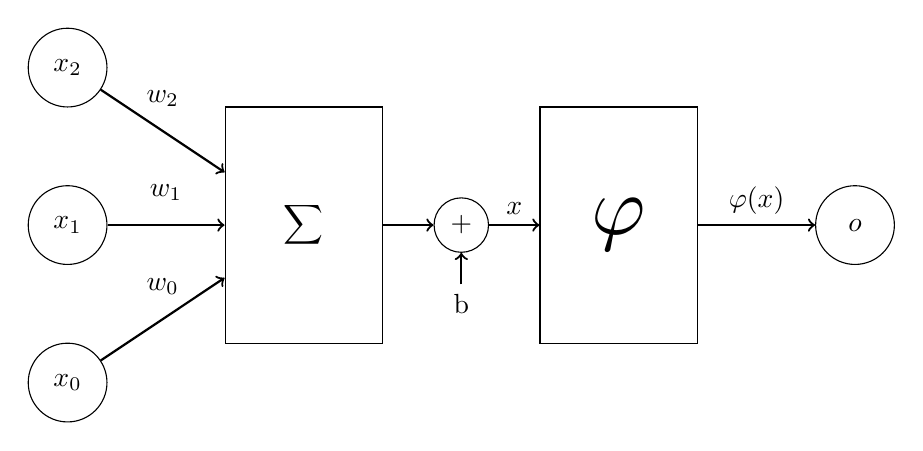
\begin{tikzpicture}

  \node[rectangle, draw=black, minimum size=2cm,minimum height=3cm] (sum) at (3, 0) {$\displaystyle\sum$};

  \foreach\name in {0,1,2}{
      \pgfmathsetmacro\y{2*\name-2}
  	\node[circle, draw=black,minimum size=1cm] (input\name) at (0, \y) {$x_{\name}$};
      \draw[thick,->] (input\name) to node[yshift=5pt,above] {$w_{\name}$} (sum);
  }

  \node[rectangle, draw=black, minimum size=2cm,minimum height=3cm] (phi) at (7, 0) {};
  \node[scale=3] (phisym) at (phi.center) {$\displaystyle\varphi$};

  \node (bias) at (5, -1) {b};
  \node[circle, draw=black] (sumb) at (5, 0) {$+$};
  \draw[thick,->] (sum.east) -- (sumb.west);
  \draw[thick,->] (bias.north) -- (sumb.south);
  \draw[thick,->] (sumb.east) -- node[above] {$x$} (phi.west);
  \node[circle,draw=black,minimum size=1cm] (out) at (10,0) {$o$};
  \draw[thick,->] (phi.east) -- node[above] {$\varphi(x)$} (out.west);
  \end{tikzpicture}
\end{document}


  }
\caption{Modélisation d'un neurone artificiel.}
\label{fig:neurone}
\end{figure}

\begin{figure}[t]
  \begin{subfigure}[b]{0.5\textwidth}
    \resizebox{\textwidth}{!}{
    \documentclass{standalone}
\usepackage[utf8]{inputenc}
\usepackage[T1]{fontenc}
\usepackage{tikz}
%%%%%%%%%%%%%%%%%%%%%%%%%%%%%%%%%%%%%%%%
%           Commandes perso            %
%%%%%%%%%%%%%%%%%%%%%%%%%%%%%%%%%%%%%%%%

%% Figures centrées, et en position 'here, top, bottom or page'
\newenvironment{figureth}{%
		\begin{figure}[htbp]
			\centering
	}{
		\end{figure}
		}


%% Tableaux centrés, et en position 'here, top, bottom or page'
\newenvironment{tableth}{%
		\begin{table}[htbp]
			\centering
			%\rowcolors{1}{coleurtableau}{coleurtableau}
	}{
		\end{table}
		}

%% Sous-figures centrées, en position 'top'
\newenvironment{subfigureth}[1]{%
	\begin{subfigure}[t]{#1}
	\centering
}{
	\end{subfigure}
}

\newcommand{\citationChap}[2]{%
	\epigraph{\og \textit{#1} \fg{}}{#2}
}

%% On commence par une page impaire quand on change le style de numérotation de pages
\let\oldpagenumbering\pagenumbering
\renewcommand{\pagenumbering}[1]{%
	\cleardoublepage
	\oldpagenumbering{#1}
}

%% Légende du dataset ISPRS
\newcommand\isprslegende{
Légende\,: \textcolor{Black}{blanc}\,: routes, \textcolor{Blue}{bleu}\,: bâtiments, \textcolor{Cerulean}{cyan}\,: végétation basse, \textcolor{OliveGreen}{vert}\,: arbres, \textcolor{Dandelion}{jaune}\,: véhicules, \textcolor{BrickRed}{rouge}\,: autre.
}

%% Dessiner des réseaux de neurones avec Tikz
\newcommand{\convlayer}[9]{%{h}{w}{d}{name}{color}{x}{y}{z}%{note w}{note h}{note d}
   \def\h{#1}
   \def\w{#2}
   \def\d{#3}
   \def\name{#4}
   \ifthenelse {\equal{#5} {}} {\def\col{white}} {\def\col{#5}}
   \def\x{#6}
   \ifthenelse {\equal{#7} {}} {\def\y{0}} {\def\y{#7}}
   \ifthenelse {\equal{#8} {}} {\def\z{0}} {\def\z{#8}}
   % ne faites pas ça chez vous !
   \ifthenelse {\equal{#9} {}} {\convlayercontinued{}{}{}} {\convlayercontinued#9}
}

\newcommand\convlayercontinued[3]{
   \def\notew{#1}
   \def\noteh{#2}
   \def\noted{#3}
   \coordinate (A) at (\x-\d/2,  \y-\h/2, \z-\w/2);
   \coordinate (B) at (\x-\d/2,  \y-\h/2, \z+\w/2);
   \coordinate (C) at (\x-\d/2,  \y+\h/2, \z+\w/2);
   \coordinate (D) at (\x-\d/2,  \y+\h/2, \z-\w/2);
   \coordinate (E) at (\x+\d/2,  \y-\h/2, \z-\w/2);
   \coordinate (F) at (\x+\d/2,  \y-\h/2, \z+\w/2);
   \coordinate (G) at (\x+\d/2,  \y+\h/2, \z+\w/2);
   \coordinate (H) at (\x+\d/2,  \y+\h/2, \z-\w/2);

    \draw [draw opacity=0.3, fill opacity=0.8, fill=\col!60!white] (A) -- (B) -- (C) -- (D) -- cycle;
    \draw [draw opacity=0.3, fill opacity=0.8, fill=\col!60!white] (A) -- (B) -- (F) -- (E) -- cycle;
    % Face haut
    %\draw [left color=\col!60!white, right color=\col!80!white, shading=axis, shading angle=180] (C) -- (D)  -- (H) -- (G) -- cycle;
    \draw [fill opacity=0.9, fill=\col!70!white] (C) -- node[rotate=45,above] {\small \name} (D) -- (H) -- (G) -- cycle;
    %\draw [fill opacity=0.9, fill=\col!70!white] (C) -- (D) -- node[above] {\small \name} (H) -- (G) -- cycle;
    % Face droite
    \draw [fill opacity=0.9, fill=\col!60!white] (E) -- node[pos=0.75,rotate=45,below] {\scriptsize \notew} (F) -- (G) --  (H) -- cycle;
    % Face avant
    %\draw [shading=axis, left color=\col!60!white, right color=\col!40!white, shading angle=-45] (B) -- node[above,rotate=90] {\scriptsize \noteh} (C) -- (G) -- (F) -- node[below] {\scriptsize \noted}  cycle;
    \draw [fill opacity=0.9, fill=\col!50!white] (B) -- node[above,rotate=90] {\scriptsize \noteh} (C) -- (G) -- (F) -- node[below] {\scriptsize \noted}  cycle;
}

\newcommand{\fclayer}[8]{%{h}{w}{name}{color}{x}{y}{z}
   \def\h{#1}
   \def\w{#2}
   \def\name{#3}
   \ifthenelse {\equal{#4} {}} {\def\col{white}} {\def\col{#4}}
   \def\x{#5}
   \def\y{#6}
   \def\z{#7}
   \def\note{#8}
   \coordinate (A) at (\x-\w/2,  \y-\h/2, \z);
   \coordinate (B) at (\x+\w/2,  \y-\h/2, \z);
   \coordinate (C) at (\x+\w/2,  \y+\h/2, \z);
   \coordinate (D) at (\x-\w/2,  \y+\h/2, \z);

   \pgfmathparse{4*\w}\let\boxwidth\pgfmathresult
    \draw [fill=\col] (A) -- node[below,text width=\boxwidth cm,align=center] {\scriptsize \note} (B) -- (C) -- (D) -- cycle;

    \node (N) at ($(A)!0.5!(B)+(0,-1,0)$) {\name};
}

\newcommand{\alexnet}[4]{%{scale}{x}{y}{z}
  \def\scale{#1}
  \def\alexx{#2}
  \def\alexy{#3}
  \def\alexz{#4}


  \def\coblue{blue!50!white}
  \def\fcgrey{gray!50!white}

  \convlayer{1.3*\scale}{1.3*\scale}{0.02*\scale}{Image}{\coblue}{\alexx}{\alexy}{\alexz}{{227}{227}{3}}
  \convlayer{1.1*\scale}{1.1*\scale}{0.08*\scale}{Conv1}{\coblue}{\alexx+0.7*\scale}{\alexy}{\alexz}{{55}{55}{96}}
  \convlayer{0.7*\scale}{0.7*\scale}{0.5*\scale}{Conv2}{\coblue}{\alexx+1.5*\scale}{\alexy}{\alexz}{{27}{27}{256}}
  \convlayer{0.5*\scale}{0.5*\scale}{0.8*\scale}{Conv3}{\coblue}{\alexx+2.6*\scale}{\alexy}{\alexz}{{13}{13}{384}}
  \convlayer{0.5*\scale}{0.5*\scale}{0.8*\scale}{Conv4}{\coblue}{\alexx+3.8*\scale}{\alexy}{\alexz}{{13}{13}{384}}
  \convlayer{0.5*\scale}{0.5*\scale}{0.5*\scale}{Conv5}{\coblue}{\alexx+4.8*\scale}{\alexy}{\alexz}{{13}{13}{256}}
  \fclayer{\scale}{0.1*\scale}{FC1}{\fcgrey}{\alexx+5.4*\scale}{\alexy}{\alexz}{4096}
  \fclayer{\scale}{0.1*\scale}{FC2}{\fcgrey}{\alexx+5.7*\scale}{\alexy}{\alexz}{4096}
  \fclayer{\scale}{0.1*\scale}{FC3}{\fcgrey}{\alexx+6.0*\scale}{\alexy}{\alexz}{1000}
}

\newcommand{\imagelayer}[7]{%{width}{x}{y}{z}{path}{text_up}{text_down}
    \pgfmathparse{#1}\let\w\pgfmathresult
    \begin{scope}[canvas is yz plane at x=#2]
     \node[transform shape] (source) at (#3, #4) {\includegraphics[angle=-90,width=\w cm]{#5}};
    \end{scope}
     \node [transform shape, rotate=45, above] at (source.east) {#6};
     \node [transform shape, rotate=45, below] at (source.west) {\scriptsize{#7}};
}

\def\fourier{\mathcal{F}}

\newcommand{\lightspectrum}{%
\pgfplotsset{
    % this *defines* a custom colormap ...
    colormap={slategraywhite}{color(0cm)=(red); color(1cm)=(red); color(2cm)=(red); color(3cm)=(red); color(4cm)=(orange); color(5cm)=(yellow); color(6cm)=(green); color(7cm)=(blue); color(8cm)=(blue); color(9cm)=(purple); color(10cm)=(purple); color(12cm)=(black)}
}
\node at (1.5, 2.7) {\small 1mm};
\node at (4, 3) {Infrarouge};
\node at (7.75, 2.7) {\small 800nm};
\node at (9, 3) {Visible};
\node at (10.5, 2.7) {\small 400nm};
\node at (12, 3) {Ultraviolet};
\node at (13.5, 2.7) {\small 10nm};
\draw[->] (1, 2.5) -- (14, 2.5);
\begin{axis}[hide axis,width=16cm,height=4cm,colormap name=slategraywhite]
\addplot[domain=20:1000,samples=1500,ultra thick, point meta=x*x,mesh]{sin(x*x/80)};
\end{axis}
}

% Union généralisée
\newcommand{\wbigcup}{\mathop{\bigcup}\displaylimits}

\newcommand{\res}[2]{#1 {\footnotesize $\pm$ #2}}
\newcommand{\bres}[2]{\textbf{#1} {\footnotesize $\pm$ #2}}
\newcommand{\bbres}[2]{\res{\textit{#1}}{#2}}

\newcommand{\drawkernel}[9]{
\begin{tikzpicture}
	\draw[step=1cm,gray!50!white,very thin] (0,0) grid (3,3);
	\kernelnode{0.5}{0.5}{#1};
	\kernelnode{0.5}{1.5}{#2};
	\kernelnode{0.5}{2.5}{#3};
	\kernelnode{1.5}{0.5}{#4};
	\kernelnode{1.5}{1.5}{#5};
	\kernelnode{1.5}{2.5}{#6};
	\kernelnode{2.5}{0.5}{#7};
	\kernelnode{2.5}{1.5}{#8};
	\kernelnode{2.5}{2.5}{#9};
\end{tikzpicture}
}

\newcommand{\kernelnode}[3]{%{x}{y}{value}
	\ifthenelse{\equal{#3}{0}}{
		\def\kcolor{gray}
	}{
		\def\kcolor{black}
	}
	\node[\kcolor] at (#1, #2) {#3};
}

\newcommand{\chapsummary}[1]{
\section*{Résumé du chapitre :}
\parbox{0.9\linewidth}{
\setlength{\parindent}{4ex}
#1}
}

\newcommand{\eqname}[1]{\tag*{\small (#1)}}

\begin{document}
  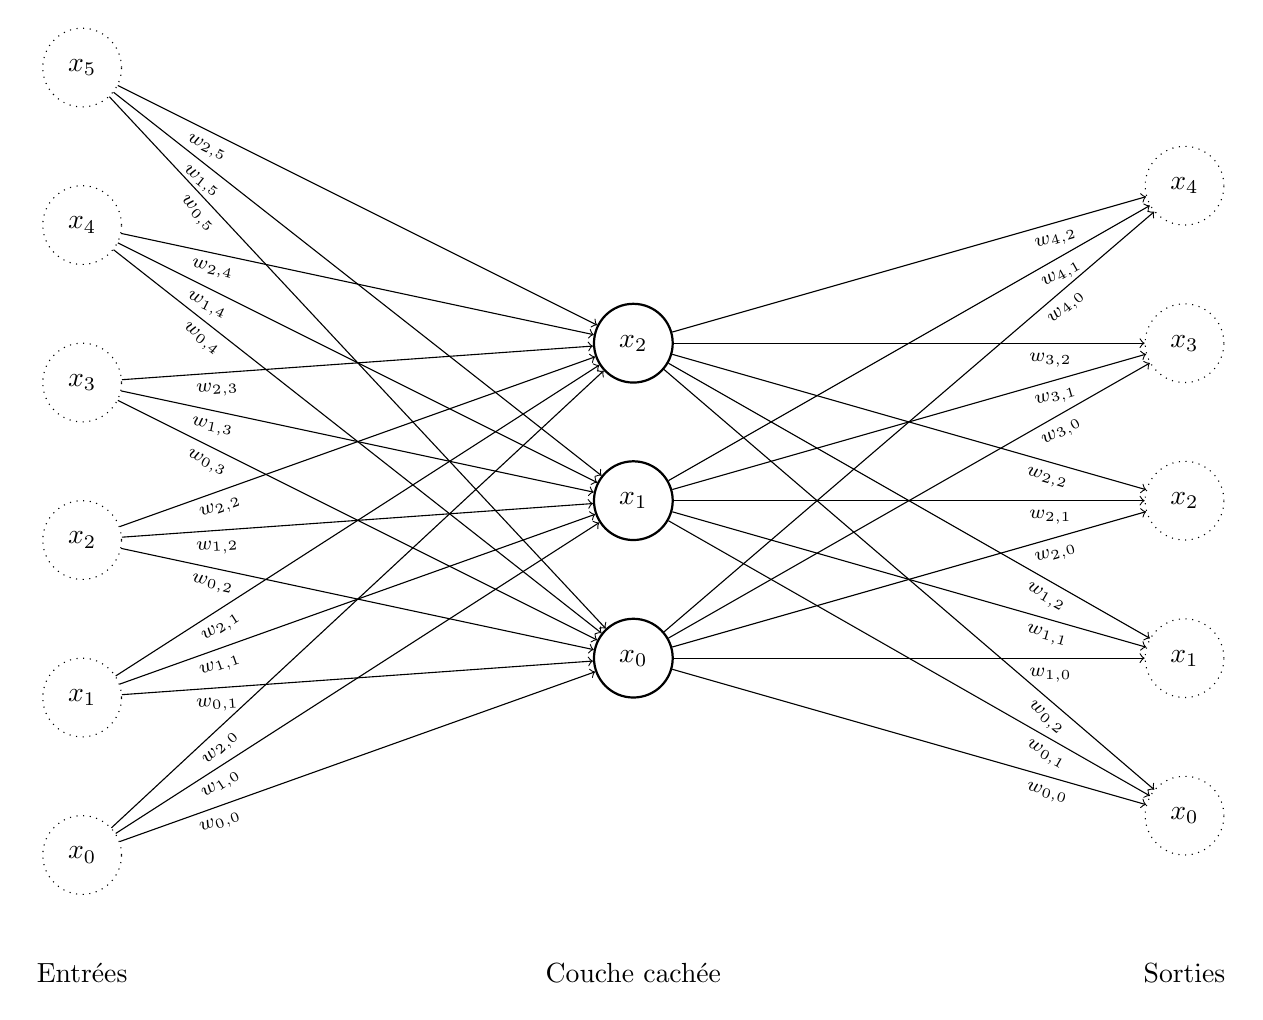
\begin{tikzpicture}
  \foreach\name in {0,1,2,3,4}{
      \pgfmathsetmacro\y{2*\name-3}
  	\node[circle, dotted,draw=black,minimum size=1cm] (output\name) at (7, \y) {$x_{\name}$};
  %    \draw[thick,->] (input\name) to node[yshift=5pt,above] {$w_{\name}$} (sum);
  }

  \foreach\name in {0,1,2}{
      \pgfmathsetmacro\y{2*\name-1}
  	\node[circle, thick,draw=black,minimum size=1cm] (hidden\name) at (0, \y) {$x_{\name}$};
      \foreach\oname in {0,1,2,3,4}{
      \draw[->] (hidden\name) to node[near end, sloped,pos=0.8,below] {\scriptsize $w_{\oname,\name}$} (output\oname);
      }
  }

  \node at (-7, -5) {Entrées};
  \node at (0, -5) {Couche cachée};
  \node at (7, -5) {Sorties};

  \foreach\name in {0,1,2,3,4,5}{
      \pgfmathsetmacro\y{2*\name-3.5}
  	\node[circle, dotted, draw=black,minimum size=1cm] (input\name) at (-7, \y) {$x_{\name}$};
      \foreach\hname in {0,1,2}{
      \draw[->] (input\name) to node[near end, sloped,pos=0.2,below] {\scriptsize $w_{\hname,\name}$} (hidden\hname);
      }
  }
  \end{tikzpicture}
\end{document}

    }
  \caption{Perceptron à une couche cachée.}
  \end{subfigure}%
  \begin{subfigure}[b]{0.5\textwidth}
    \resizebox{\textwidth}{!}{
    \documentclass{standalone}
\usepackage[utf8]{inputenc}
\usepackage[T1]{fontenc}
\usepackage{tikz}
\usepackage{ifthen}
%%%%%%%%%%%%%%%%%%%%%%%%%%%%%%%%%%%%%%%%
%           Commandes perso            %
%%%%%%%%%%%%%%%%%%%%%%%%%%%%%%%%%%%%%%%%

%% Figures centrées, et en position 'here, top, bottom or page'
\newenvironment{figureth}{%
		\begin{figure}[htbp]
			\centering
	}{
		\end{figure}
		}


%% Tableaux centrés, et en position 'here, top, bottom or page'
\newenvironment{tableth}{%
		\begin{table}[htbp]
			\centering
			%\rowcolors{1}{coleurtableau}{coleurtableau}
	}{
		\end{table}
		}

%% Sous-figures centrées, en position 'top'
\newenvironment{subfigureth}[1]{%
	\begin{subfigure}[t]{#1}
	\centering
}{
	\end{subfigure}
}

\newcommand{\citationChap}[2]{%
	\epigraph{\og \textit{#1} \fg{}}{#2}
}

%% On commence par une page impaire quand on change le style de numérotation de pages
\let\oldpagenumbering\pagenumbering
\renewcommand{\pagenumbering}[1]{%
	\cleardoublepage
	\oldpagenumbering{#1}
}

%% Légende du dataset ISPRS
\newcommand\isprslegende{
Légende\,: \textcolor{Black}{blanc}\,: routes, \textcolor{Blue}{bleu}\,: bâtiments, \textcolor{Cerulean}{cyan}\,: végétation basse, \textcolor{OliveGreen}{vert}\,: arbres, \textcolor{Dandelion}{jaune}\,: véhicules, \textcolor{BrickRed}{rouge}\,: autre.
}

%% Dessiner des réseaux de neurones avec Tikz
\newcommand{\convlayer}[9]{%{h}{w}{d}{name}{color}{x}{y}{z}%{note w}{note h}{note d}
   \def\h{#1}
   \def\w{#2}
   \def\d{#3}
   \def\name{#4}
   \ifthenelse {\equal{#5} {}} {\def\col{white}} {\def\col{#5}}
   \def\x{#6}
   \ifthenelse {\equal{#7} {}} {\def\y{0}} {\def\y{#7}}
   \ifthenelse {\equal{#8} {}} {\def\z{0}} {\def\z{#8}}
   % ne faites pas ça chez vous !
   \ifthenelse {\equal{#9} {}} {\convlayercontinued{}{}{}} {\convlayercontinued#9}
}

\newcommand\convlayercontinued[3]{
   \def\notew{#1}
   \def\noteh{#2}
   \def\noted{#3}
   \coordinate (A) at (\x-\d/2,  \y-\h/2, \z-\w/2);
   \coordinate (B) at (\x-\d/2,  \y-\h/2, \z+\w/2);
   \coordinate (C) at (\x-\d/2,  \y+\h/2, \z+\w/2);
   \coordinate (D) at (\x-\d/2,  \y+\h/2, \z-\w/2);
   \coordinate (E) at (\x+\d/2,  \y-\h/2, \z-\w/2);
   \coordinate (F) at (\x+\d/2,  \y-\h/2, \z+\w/2);
   \coordinate (G) at (\x+\d/2,  \y+\h/2, \z+\w/2);
   \coordinate (H) at (\x+\d/2,  \y+\h/2, \z-\w/2);

    \draw [draw opacity=0.3, fill opacity=0.8, fill=\col!60!white] (A) -- (B) -- (C) -- (D) -- cycle;
    \draw [draw opacity=0.3, fill opacity=0.8, fill=\col!60!white] (A) -- (B) -- (F) -- (E) -- cycle;
    % Face haut
    %\draw [left color=\col!60!white, right color=\col!80!white, shading=axis, shading angle=180] (C) -- (D)  -- (H) -- (G) -- cycle;
    \draw [fill opacity=0.9, fill=\col!70!white] (C) -- node[rotate=45,above] {\small \name} (D) -- (H) -- (G) -- cycle;
    %\draw [fill opacity=0.9, fill=\col!70!white] (C) -- (D) -- node[above] {\small \name} (H) -- (G) -- cycle;
    % Face droite
    \draw [fill opacity=0.9, fill=\col!60!white] (E) -- node[pos=0.75,rotate=45,below] {\scriptsize \notew} (F) -- (G) --  (H) -- cycle;
    % Face avant
    %\draw [shading=axis, left color=\col!60!white, right color=\col!40!white, shading angle=-45] (B) -- node[above,rotate=90] {\scriptsize \noteh} (C) -- (G) -- (F) -- node[below] {\scriptsize \noted}  cycle;
    \draw [fill opacity=0.9, fill=\col!50!white] (B) -- node[above,rotate=90] {\scriptsize \noteh} (C) -- (G) -- (F) -- node[below] {\scriptsize \noted}  cycle;
}

\newcommand{\fclayer}[8]{%{h}{w}{name}{color}{x}{y}{z}
   \def\h{#1}
   \def\w{#2}
   \def\name{#3}
   \ifthenelse {\equal{#4} {}} {\def\col{white}} {\def\col{#4}}
   \def\x{#5}
   \def\y{#6}
   \def\z{#7}
   \def\note{#8}
   \coordinate (A) at (\x-\w/2,  \y-\h/2, \z);
   \coordinate (B) at (\x+\w/2,  \y-\h/2, \z);
   \coordinate (C) at (\x+\w/2,  \y+\h/2, \z);
   \coordinate (D) at (\x-\w/2,  \y+\h/2, \z);

   \pgfmathparse{4*\w}\let\boxwidth\pgfmathresult
    \draw [fill=\col] (A) -- node[below,text width=\boxwidth cm,align=center] {\scriptsize \note} (B) -- (C) -- (D) -- cycle;

    \node (N) at ($(A)!0.5!(B)+(0,-1,0)$) {\name};
}

\newcommand{\alexnet}[4]{%{scale}{x}{y}{z}
  \def\scale{#1}
  \def\alexx{#2}
  \def\alexy{#3}
  \def\alexz{#4}


  \def\coblue{blue!50!white}
  \def\fcgrey{gray!50!white}

  \convlayer{1.3*\scale}{1.3*\scale}{0.02*\scale}{Image}{\coblue}{\alexx}{\alexy}{\alexz}{{227}{227}{3}}
  \convlayer{1.1*\scale}{1.1*\scale}{0.08*\scale}{Conv1}{\coblue}{\alexx+0.7*\scale}{\alexy}{\alexz}{{55}{55}{96}}
  \convlayer{0.7*\scale}{0.7*\scale}{0.5*\scale}{Conv2}{\coblue}{\alexx+1.5*\scale}{\alexy}{\alexz}{{27}{27}{256}}
  \convlayer{0.5*\scale}{0.5*\scale}{0.8*\scale}{Conv3}{\coblue}{\alexx+2.6*\scale}{\alexy}{\alexz}{{13}{13}{384}}
  \convlayer{0.5*\scale}{0.5*\scale}{0.8*\scale}{Conv4}{\coblue}{\alexx+3.8*\scale}{\alexy}{\alexz}{{13}{13}{384}}
  \convlayer{0.5*\scale}{0.5*\scale}{0.5*\scale}{Conv5}{\coblue}{\alexx+4.8*\scale}{\alexy}{\alexz}{{13}{13}{256}}
  \fclayer{\scale}{0.1*\scale}{FC1}{\fcgrey}{\alexx+5.4*\scale}{\alexy}{\alexz}{4096}
  \fclayer{\scale}{0.1*\scale}{FC2}{\fcgrey}{\alexx+5.7*\scale}{\alexy}{\alexz}{4096}
  \fclayer{\scale}{0.1*\scale}{FC3}{\fcgrey}{\alexx+6.0*\scale}{\alexy}{\alexz}{1000}
}

\newcommand{\imagelayer}[7]{%{width}{x}{y}{z}{path}{text_up}{text_down}
    \pgfmathparse{#1}\let\w\pgfmathresult
    \begin{scope}[canvas is yz plane at x=#2]
     \node[transform shape] (source) at (#3, #4) {\includegraphics[angle=-90,width=\w cm]{#5}};
    \end{scope}
     \node [transform shape, rotate=45, above] at (source.east) {#6};
     \node [transform shape, rotate=45, below] at (source.west) {\scriptsize{#7}};
}

\def\fourier{\mathcal{F}}

\newcommand{\lightspectrum}{%
\pgfplotsset{
    % this *defines* a custom colormap ...
    colormap={slategraywhite}{color(0cm)=(red); color(1cm)=(red); color(2cm)=(red); color(3cm)=(red); color(4cm)=(orange); color(5cm)=(yellow); color(6cm)=(green); color(7cm)=(blue); color(8cm)=(blue); color(9cm)=(purple); color(10cm)=(purple); color(12cm)=(black)}
}
\node at (1.5, 2.7) {\small 1mm};
\node at (4, 3) {Infrarouge};
\node at (7.75, 2.7) {\small 800nm};
\node at (9, 3) {Visible};
\node at (10.5, 2.7) {\small 400nm};
\node at (12, 3) {Ultraviolet};
\node at (13.5, 2.7) {\small 10nm};
\draw[->] (1, 2.5) -- (14, 2.5);
\begin{axis}[hide axis,width=16cm,height=4cm,colormap name=slategraywhite]
\addplot[domain=20:1000,samples=1500,ultra thick, point meta=x*x,mesh]{sin(x*x/80)};
\end{axis}
}

% Union généralisée
\newcommand{\wbigcup}{\mathop{\bigcup}\displaylimits}

\newcommand{\res}[2]{#1 {\footnotesize $\pm$ #2}}
\newcommand{\bres}[2]{\textbf{#1} {\footnotesize $\pm$ #2}}
\newcommand{\bbres}[2]{\res{\textit{#1}}{#2}}

\newcommand{\drawkernel}[9]{
\begin{tikzpicture}
	\draw[step=1cm,gray!50!white,very thin] (0,0) grid (3,3);
	\kernelnode{0.5}{0.5}{#1};
	\kernelnode{0.5}{1.5}{#2};
	\kernelnode{0.5}{2.5}{#3};
	\kernelnode{1.5}{0.5}{#4};
	\kernelnode{1.5}{1.5}{#5};
	\kernelnode{1.5}{2.5}{#6};
	\kernelnode{2.5}{0.5}{#7};
	\kernelnode{2.5}{1.5}{#8};
	\kernelnode{2.5}{2.5}{#9};
\end{tikzpicture}
}

\newcommand{\kernelnode}[3]{%{x}{y}{value}
	\ifthenelse{\equal{#3}{0}}{
		\def\kcolor{gray}
	}{
		\def\kcolor{black}
	}
	\node[\kcolor] at (#1, #2) {#3};
}

\newcommand{\chapsummary}[1]{
\section*{Résumé du chapitre :}
\parbox{0.9\linewidth}{
\setlength{\parindent}{4ex}
#1}
}

\newcommand{\eqname}[1]{\tag*{\small (#1)}}

\begin{document}

    \begin{tikzpicture}

    \newcommand\drawlayer[7]{%{nombre de neurones}{position en x}{symbole}{nom de la couche}{couche précédente}{n couche précédente}{style}
      \foreach\name in {0,...,#1}{
        \pgfmathsetmacro\y{2*(\name-#1/2)}
      	\node[circle,#7,draw=black,minimum size=1cm] (#4_\name) at (#2, \y) {$#3_{\name}$};
          \ifthenelse{\equal{#5}{}}{}{
		\foreach\oname in {0,...,#6}{
	            {\draw[->] (#5_\oname) to (#4_\name);}
         	 }
      	  }
      }
    }

    \drawlayer{5}{0}{x}{input}{}{}{dotted}
    \drawlayer{3}{4}{h^1}{hidden1}{input}{5}{thick}
    \drawlayer{4}{8}{h^2}{hidden2}{hidden1}{3}{thick}
    \drawlayer{3}{12}{h^3}{hidden3}{hidden2}{4}{thick}
    \drawlayer{3}{16}{y}{output}{hidden3}{3}{dotted}

    \node at (0,-6.5) {Entrées};
    \node at (8,-6.5) {Couches cachées};
    \node at (16,-6.5) {Sorties};

    \end{tikzpicture}

\end{document}


    }
  \caption{Perceptron multi-couches.}
  \end{subfigure}
  \caption{Perceptron à une et plusieurs couches. Les entrées et sorties peuvent être de dimensions variables et sont représentées comme des neurones.}
  \label{fig:perceptron}
\end{figure}

La définition formelle d'un neurone artificiel a été introduite par McCulloch et Pitts~\cite{lettvin_what_1959} en 1959. Un neurone doté d'une fonction de transfert $\varphi$ opère sur un ensemble de $n$ neurones d'entrée émettant chacun une valeur $x_1\dots{}x_n$, auxquelles il est connecté par des synapses de poids $w_i$. La valeur d'entrée $x$ du neurone correspond à la somme pondérée des signaux d'entrée. Le neurone émet ensuite l'image $z = \varphi(x)$ de ce signal par sa fonction de transfert. Le schéma de la~\cref{fig:neurone} décrit ce procédé. L'activation en sortie d'un neurone s'obtient donc par la formule
$$z = \varphi\left(\sum_{i=1}^n w_i x_i + b\right)~.$$

Plusieurs neurones connectés les uns aux autres forment un graphe orienté et pondéré. Un réseau de neurones à propagation avant désigne un graphe neuronal acyclique. En pratique, on considère des graphes multipartis que l'on peut alors représenter par \fg couches \og{}. Dans le cas d'un perceptron à couches multiples, les valeurs du signal d'entrée sont placées dans une couche d'entrée et les signaux de sortie envoyés dans une couche de sortie. La ou les couches de neurones réellement optimisables sont nommées \og couches cachées \fg{} et font l'interface entre l'entrée et la sortie. Le perceptron multi-couches à une et plusieurs couches cachées sont illustrés dans la~\cref{fig:perceptron}.

La fonction d'activation des neurones peut prendre de nombreuses formes. Il est \emph{a minima} nécessaire que celle-ci soit non-linéaire, sans quoi elle rend le perceptron multi-couches équivalent au perceptron simple, et presque partout différentiable afin de pouvoir appliquer l'algorithme de rétropropagation du gradient. La fonction d'activation est en outre généralement choisie monotone croissante et de dérivée monotone croissante. La~\cref{fig:activations} illustre plusieurs activations communément utilisées dans les réseaux de neurones artificiels profonds\,:
\begin{itemize}
  \item La \textbf{sigmoïde}, ou fonction logistique\,: $\sigma(x) = \frac{1}{1 + e^{-x}}$.
  \item La fonction \textbf{tangente hyperbolique}\,: $\tanh(x) = \frac{1 - e^{-2x}}{1 + e^{-2x}}$.
  \item La \textbf{marche de Heavyside}\,: $H(x) = 0 \text{ si } x < 0 \text{ et } 1 \text{ si } x \geq 0$.
  \item La fonction \textbf{\gls{ReLU}}\,: $ReLU(x) = max(0,x)$.
  \item La fonction \textbf{SoftPlus}\,: $s(x) = ln(1 + e^x)$.
\end{itemize}

\begin{figure}[t]
  \begin{subfigure}[b]{0.5\textwidth}
    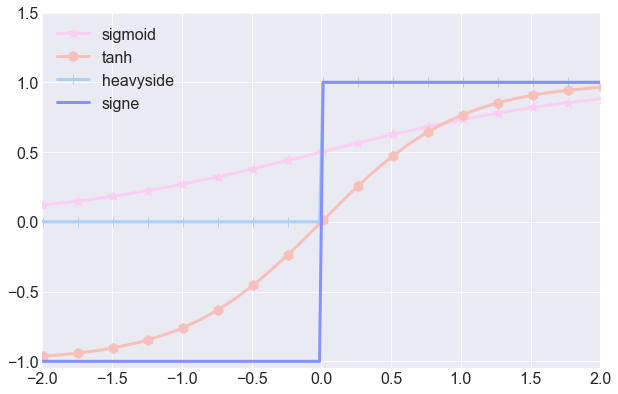
\includegraphics[width=\textwidth]{activations}
    \caption{Fonctions d'activation saturantes.}
    \label{fig:activations}
  \end{subfigure}
\begin{subfigure}[b]{0.5\textwidth}
  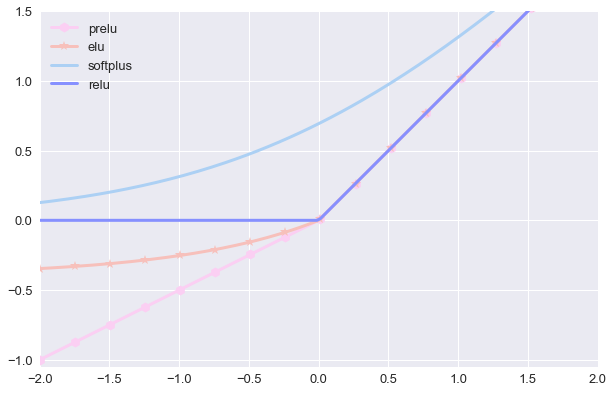
\includegraphics[width=\textwidth]{rectifiers}
  \caption{Fonctions d'activation non-saturantes.}
  \label{fig:rectifiers}
\end{subfigure}
\caption{Exemples de fonctions d'activation.}
\label{fig:activations}
\end{figure}

La fonction sigmoïde, bien que populaire à l'origine, est une fonction saturante qui souffre de gradients évanescents. Ce problème n'est pas circonscrit à la sigmoïde et est particulièrement pregnant dans le cas des réseaux de neurones récurrents~\cite{hochreiter_gradient_2001}. L'accumulation de couches dans un réseau fait que la rétropropagation du gradient est similaire à une suite géométrique. Le produit cumulé de $n$ gradients dans des fonctions d'activation à tendance contractante produit un $n+1$ gradient plus faible que le précédent, et ainsi de suite. À l'inverse, il est possible d'avoir des gradients explosifs. Ce problème est empiré dans le cas des fonctions saturants comme la sigmoïde ou la tangente hyperbolique car leurs gradients sont nécessairement dans $[0,1]$. L'utilisation de la sigmoïde ou la tangente hyperbolique a varié dans la littérature. LeCun~\cite{lecun_efficient_1998} recommande d'utiliser la fonction hyperbolique modifiée $f(x) = 1,7159 tanh(\frac{2}{3} x)$, notamment car celle-ci est bornée par $[-1,1]$ et centrée en 0, ce qui est adapté au travail sur des données normalisées à moyenne nulle et variance unitaire.

La marche de Heavyside, tout comme la fonction $signe$, a des gradients nuls presque partout, sa dérivée étant l'impulsion de Dirac $\delta$.

Pour limiter les gradients évanescents, des fonctions non-linéaires non-saturantes sont désormais majoritairement utilisées dans la littérature. Glorot, Bordes et Bengio~\cite{glorot_deep_2011} ont ainsi proposé d'utiliser la fonction \gls{ReLU}, introduite précédemment pour les \gls{DBN}~\cite{nair_rectified_2010}, et la fonction SoftPlus pour les réseaux de neurones artificiels de toutes sortes. Leurs travaux aboutissent à trois conclusions importantes. Tout d'abord, les fonctions d'activation non-linéaire obtiennent généralement de meilleures performances que les réseaux utilisant $tanh$. Ensuite, les réseaux entraînés avec \gls{ReLU} ne nécessitent pas de pré-apprentissage non-supervisé couche par couche, ce qui accélère grandement les temps d'entraînement. Enfin, ces modèles sont plus parcimonieux que leurs équivalents usuels. En outre, la fonction \gls{ReLU} est simple à implémenter et rapide à calculer, ce qui a contribué à sa popularisation rapide dans la communauté.

Plusieurs variantes ont dès lors été proposées autour des fonctions linéaires rectifiées, notamment une version paramétrique dont la partie négative est non-saturante, mais linéaire de pente $\alpha$ fixée par l'utilisateur (\emph{Leaky ReLU}~\cite{maas_rectifier_2013}) ou optimisable (\gls{PReLU}~\cite{he_delving_2015}). Une version similaire mais continue a également été proposée sous la forme des \gls{ELU}~\cite{clevert_fast_2015}. Plus récemment, une recherche automatique quasi-exhaustive sur une variété de fonctions d'activation possibles a permis de proposer la \emph{Swish}~\cite{ramachandran_searching_2018}, non-linéaire non-saturante mais ayant la particularité d'être non-monotone. Ces variantes sont illustrées dans la~\cref{fig:rectifiers} et leur formule est donnée ci-dessous\,:
\begin{itemize}
  \item La fonction \textbf{\emph{Leaky ReLU}}\,: $LReLU_\alpha(x) = max(0,x) - \alpha max(0,-x)$, avec $\alpha$ un hyperparamètre.
  \item La fonction \textbf{\gls{PReLU}}\,: $PReLU(x, \alpha) = max(0,x) - \alpha max(0,-x)$, avec $\alpha$ optimisable.
  \item La fonction \textbf{\gls{ELU}}\,: $ELU_\alpha(x) = x \text{ si } x > 0 \text{ et } \alpha (exp(x) - 1) \text{ sinon}$.
  \item La fonction \textbf{\emph{Swish}}\,: $Swish_\beta(x) = x . \sigma(\beta x) = x . (1 + e^{-\beta x})^{-1}$.
\end{itemize}
% TODO : ref Oyallon sur les "bonnes" hypothèses pour la fonction d'activation

Le théorème d'approximation universelle~\cite{cybenko_approximation_1989,hornik_approximation_1991} indique que l'ensemble des fonctions engendrées par les perceptrons est dense dans l'ensemble des fonctions continues par morceaux sur des compacts. Autrement dit, toute fonction $f : E \rightarrow \mathbb{R}^m$ avec $E = \bigcup\limits_{k} C_k$ une union de compacts de $\mathbb{R}^n$ continue sur chaque compact est approximable à une précision $\epsilon$ arbitraire par un perceptron. On peut voir deux limitations à ce résultat. Le premier concerne la nature de la fonction d'activation. Le théorème généralisé par Hornik s'applique à tous les perceptrons sur lesquels on applique une fonction d'activation monotone non-constante et bornée, cela couvre les fonctions saturantes $tanh$ et sigmoide, mais exclut les fonctions linéaires rectifiées comme \gls{ReLU}. Ce problème a cependant été levé par Sonoda et Murata~\cite{sonoda_neural_2017}, qui ont montré que des réseaux munis de fonctions d'activation non-bornées satisfaient tout de même le théorème d'approximation universelle


La deuxième limitation porte quant à elle sur la nature même du théorème. Celui-ci ne donne qu'une garantie purement théorique concernant l'existence d'un ensemble de paramètres permettant l'approximation à la précision voulue. Il ne donne pas de bornes sur le nombre de neurones nécessaire, ni de méthode de construction. Ainsi, il n'y aucune certitude que les poids puissent être obtenus par descente de gradient, ni d'indication sur l'architecture à choisir. En particulier, le théorème vaut pour des réseaux superficiels à une seule couche. Pourtant, le consensus scientifique dans la communauté tend à préférer des réseaux de plus en plus profonds. Ainsi, il a été démontré que des réseaux plus profonds demandent moins de poids et de neurones pour approximer des fonctions plus complexes~\cite{bianchini_complexity_2014,mhaskar_when_2017}. En particulier, la structure hiérarchique des réseaux multi-couches semble adapté à l'approximation de fonctions composées en contournant la malédiction de la dimension~\cite{poggio_why_2017}. Toutefois, cela augmente également le nombre d'hyperparamètres à régler pour définir l'architecture. L'absence de méthode systématique de construction des architectures de réseau profond conduit donc à l'utilisation intensive de la méthode essai-erreur ou à des méthodes de méta-apprentissage~\cite{zoph_neural_2016}.

\subsection{Entraînement des réseaux de neurones}

Un autre inconvénient au théorème d'approximation universelle est que même si l'architecture était connue, celui-ci ne donne aucune méthode pour trouver les valeurs des paramètres. En particulier, l'algorithme de rétropropagation du gradient~\cite{werbos_beyond_1975,rumelhart_learning_1986,lecun_learning_1986} décrit ci-après se base sur une méthode de descente de gradient. Toutefois, rien ne garantit que les poids optimaux dont l'existence est assurée par le théorème d'approximation universelle ne soit trouvables par cet algorithme.

L'algorithme de rétropropagation du gradient se fonde sur la règle de dérivation en chaîne, c'est-à-dire le théorème de dérivation des fonctions composées~\cite{lhospital_analyse_1716,lagrange_theorie_1797}\,:
\begin{theorem}
Soient $f$ et $g$ deux fonctions telles que $f : I \rightarrow J \subset \mathbb{R}$ et $g : J \rightarrow \mathbb{R}$. Soit $x \in I$ tel que $f$ admet une dérivée en $x$. Alors, la fonction composée $h = g \circ f : I \rightarrow \mathbb{R}$ admet une dérivée en $x$ de valeur :
$$h'(x) = (g \circ f)'(x) = f'(x) \times g'(f(x))~.$$

Si $f$ et $g$ sont dérivables respectivement sur $I$ et $J$, alors\,:
$$(g \circ f)' = f' \times (g' \circ f)~.$$

ou encore, en utilisant la notation de Leibniz, avec $z = g(y)$ et $y = f(x)$:
$$\frac{\diff z}{\diff x} = \frac{\diff z}{\diff y} \times \frac{\diff y}{\diff x}~.$$
\end{theorem}

Ce théorème s'étend aux dérivées partielles de fonctions à valeurs dans $\mathbb{R}^n$.

Dans le cas des réseaux profondes, la propagation avant des activations se fait par la formule suivante\,:
$$z_j^{k+1} = \varphi\left(\sum_{i=1}^n w^k_{i,j} \cdot z^k_i + b^k_j\right)$$
avec $\varphi$ la fonction d'activation, $w_{i,j}$ le poids de la connexion, $b_i$ le biais et $k$ le numéro de la couche.

En connaissant l'erreur $e^{k+1}$, c'est-à-dire le gradient pour la couche $k+1$, alors\,:

$$e^k_j = \sum_{i=1}^N w^k_{i,j} e^{k+1}_j  \varphi'\left(\sum_{i=1}^n w^k_{i,j} \cdot z^k_i + b^k_j\right)$$

Pour diminuer l'erreur, il est nécessaire de mettre à jour les poids $w^k$ dans la direction opposée au gradient $\frac{\diff e}{\diff w^k}$. Or, grâce à la règle de la dérivation en chaîne\,:
$$\frac{\diff e}{\diff w^k} = \frac{\diff e}{\diff z^k} \times \frac{\diff z^k}{\diff w^k}$$.


On peut alors utiliser l'algorithme de descente de gradient~\cite{cauchy_comptes_1847} afin de minimiser l'erreur totale en mettant à jour les poids. Cet algorithme, dit de la plus forte pente, permet d'approcher des minima locaux d'une fonction $f$ arbitraire en cherchant ses points stationnaires, c'est-à-dire les points où le gradient de $f$ s'annule. L'algorithme repose sur l'idée que $f$ décroît le plus rapidement dans la direction opposée à son gradient et fonctionne de la façon suivante\,:

\begin{theorem}
  Soit $f : \mathbb{R}^n \rightarrow \mathbb{R}$ une fonction différentiable et $\nabla f$ son gradient. Soit $x_0 \in \mathbb{R}^n$ un point initial, $\epsilon > 0$ le seuil de tolérance de l'algorithme et $\alpha > 0$ le pas de la descente. On définit alors la suite $(x_i)_{i \ge 0} \in \mathbb{R}^\mathbb{N}$ telle que\,:
  $$x_{i+1} = x_i - \alpha \nabla f(x_i)~.$$
  L'algorithme s'arrête lorsque $\nabla f(x_i) \le \epsilon$.
\end{theorem}

Dans le cas des réseaux de neurones, la fonction $f$ est appelée \og fonction objectif \fg et correspond à une mesure de la performance du modèle. Généralement, $f$ est une indicatrice de l'erreur totale du modèle sur l'ensemble du jeu de données d'entraînement $\Omega$, que l'on va chercher à minimiser. Ainsi, l'optimisation du réseau de neurones consiste à résoudre l'équation\,:
$$W^* = \operatorname{argmin}_W E(W, \Omega)$$
 pour un modèle paramétré par ses poids $W$ et de fonction objectif $E$.

Tant que la fonction de coût $E$ est dérivable, il est possible de la minimise en utilisant l'algorithme de descente de gradient. En particulier, il est possible de calculer la mise à jour des poids en rétro-propageant la valeur du gradient d'une couche à la précédente\,: c'est l'algorithme de rétropropagation~\cite{werbos_beyond_1975,lecun_efficient_1998,rumelhart_learning_1986}. On va alors chercher à mettre à jour les poids du réseau dans la direction opposée du gradient par rapport à ces mêmes poids $\nabla_W E(W, \Omega)$.

\begin{theorem}
  \begin{enumerate}
    \item Initialiser aléatoirement les poids $W$.
    \item Calculer $\nabla_W E(W, \Omega)$ à partir de l'erreur sur chaque échantillon.
    \item Tant que $\nabla_W E(W, \Omega) > \epsilon$\,:
      \begin{itemize}
          \item $W = W - \nabla_W E(W, \Omega)$
      \end{itemize}
  \end{enumerate}
\end{theorem}

 Cependant, le cardinal de $\Omega$ peut être très grand en pratique, les bases de données d'apprentissage pouvant contenir des milliers, voire des millions d'exemple. Par conséquent, il est généralement nécessaire d'utiliser une variante en ligne de l'algorithme de gradient, l'algorithme de descente de gradient \emph{stochastique}, qui réalise la mise à jour des poids pour chaque exemple, en approximant l'erreur moyenne à partir de l'erreur sur un seul échantillon, c'est-à-dire\,:
\begin{theorem}
  \begin{enumerate}
    \item Initialiser aléatoirement les poids $W$.
    \item Tant que le critère d'arrêt n'est pas atteint\,:
      \begin{itemize}
          \item Tirer aléatoirement un exemple d'apprentissage $\omega \in \Omega$
          \item $W = W - \nabla_W E(W, \omega)$
      \end{itemize}
  \end{enumerate}
L'algorithme s'arrête lorsque le critère d'arrêt est vérifié, généralement lorsqu'un nombre d'itérations prédéfini est atteint.
\end{theorem}

L'inconvénient de l'algorithme de descente de gradient stochastique est que l'approximation du gradient $\nabla_W E(W, \omega)$ est très bruitée et peut changer fortement de direction entre deux itérations successives. Afin de stabiliser la convergence, on utilise le plus souvent l'algorithme de descente de gradient stochastique \emph{par mini-lots}, également appelés \emph{mini-batches}. On approxime alors le gradient global non pas à partir d'un échantillon, mais à partir de la moyenne sur un nombre $k$ d'échantillons, qui forment un mini-lot ou \emph{mini-batch}\,:
\begin{theorem}
  \begin{enumerate}
    \item Initialiser aléatoirement les poids $W$.
    \item Tant que le critère d'arrêt n'est pas atteint\,:
      \begin{itemize}
          \item Tirer aléatoirement $k$ exemples d'apprentissage $(\omega_1,\dots,\omega_k) \in \Omega^k$
          \item $W = W - \frac{1}{k} \sum_{i=1}^k \nabla_W E(W, \omega_i)$
      \end{itemize}
  \end{enumerate}
L'algorithme s'arrête lorsque le critère d'arrêt est vérifié, généralement lorsqu'un nombre d'itérations prédéfini est atteint.
\end{theorem}

En pratique, le modèle approxime une fonction $\mathcal{F}$ sur laquelle on applique une fonction de coût $\mathcal{L}$. Cette fonction de coût est une indicatrice de l'erreur commise par le réseau. Cette fonction doit vérifier la propriété\,:
$$\mathcal{L}(\hat{\mathcal{F_W}(x)} - \mathcal{F_W}(x)) \rightarrow 0 \Rightarrow \hat{\mathcal{F}} \rightarrow \mathcal{F}~~,$$
c'est-à-dire que la minimisation de l'erreur implique la convergence du modèle vers la fonction réelle à approximer.

La nature exacte de la fonction de coût dépend de la tâche. Dans un cadre de régression, il est courant d'utiliser la norme $L_2$ ou la norme $L_1$. Pour chaque échantillon, on pourra alors comparer la prédiction $x$ avec la vérité terrain $y$ par
$$l(x,y) = |x - y| \text{ ou } l(x,y) = \lVert x - y \rVert~~.$$
La première correspond à la méthode des moindres carrées. La norme $L_1$ se montre plus robuste aux observations aberrantes, qui explosent dans le cas de la norme euclidienne. Toutefois, la norme $L_2$ a l'avantage d'être partout dérivable et est plus stable, notamment de par sa tolérance aux faibles erreurs (fonction contractante sur $[-1, 1]$).

Dans le cas de la classification, $y$ se présente sous la forme d'un encodage \emph{one-hot}. Pour un problème à $n$ classes, si $y$ appartient à la $k$\ieme classe, alors $y_i = \delta_{i,k}$ avec $\delta$ le symbole de Kronecker. Autrement dit, $y$ est le vecteur $(0, \dots, 0, 1, 0, \dots, 0)$ dont toutes les composantes sont nulles à l'exception de la $k$\ieme qui est unitaire. S'il est possible de traiter ces problèmes avec des fonctions de coût de régression, il est généralement plus pertinent d'utiliser la fonction d'entropie croisée. Celle-ci se calcule de la façon suivante\,:
$$H(x,y) = -\sum_{i=1}^n y_i \log(x_i)~.$$

L'entropie croisée est particulièrement intéressante dans ce cas car sa minimisation coïncide avec celle de la divergence de Kullback-Leibler entre la distribution statistique des $x$ et des $y$, c'est-à-dire l'image de $\mathcal{F}$ et celle de $\hat{mathcal{F}}$.

Il est important de noter que l'algorithme de descente de gradient ne dispose d'une convergence garantie que dans le cas où la fonction $E$ est convexe, ce qui n'est jamais le cas en pratique pour des réseaux profonds. Des variantes de la descente de gradient ont été proposées pour améliorer ses propriétés de convergence. En particulier, le pas de la descente $\alpha$ joue un rôle important dans l'optimisation des réseaux de neurones profonds. Appelé généralement taux d'apprentissage, $\alpha$ contrôle à l'amplitude des mises à jour des poids du modèle. Si $\alpha$ est très élevé, les mises à jour seront très grande et la convergence très instable. Si $\alpha$ est très faible, la convergence peut être très lente voire se bloquer dans des minima locaux. La plupart des variantes de la descente de gradient stochastique utilisent des politiques particulières pour la mise à jour des poids. Des méthodes dites de \og moment \fg, inspirées du moment cinétique en mécanique, permettent notamment de faire conserver au gradient une partie de sa vélocité des itérations précédentes pour limiter les oscillations le long des courbes de niveaux de la fonction~\cite{qian_momentum_1999,nesterov_method_1983}. \citet{sutskever_importance_2013-1} ont notamment montré que l'utilisation d'une descente de gradient stochastique à moment permet d'améliorer les performances finales du modèle, y compris dans le cas d'une poids initiaux mal choisis. \citet{polyak_acceleration_1992} propose par ailleurs d'utiliser le gradient moyennée sur les $n$ dernières itérations pour la mise à jour des poids, ce qui correspond à une forme de mini-lot asynchrone.

Une autre source d'amélioration proposée réside dans la politique du choix de $\alpha$. En effet, rien ne contraint $\alpha$ à être fixé dans l'algorithme de descente de gradient. Il est possible de l'ajuster manuellement au cours de l'apprentissage, par exemple en commençant avec un taux d'apprentissage élevé au début, puis en le multipliant par un ratio $\gamma < 1$ à intervalles réguliers. \citet{bottou_stochastic_2012} recommande ainsi de la descente de gradient stochastique moyennée couplée avec une évolution de $\alpha$ suivant la relation $\alpha_{i+1} = \alpha_0 (1 + \gamma \cdot i)^{-1}$. Plus récemment, \citet{loshchilov_sgdr_2016} ont proposé une méthode à base de recuit simulé. Toutefois, cela nécessite une intervention manuelle dans la mesure où il est nécessaire de configurer un certain nombre d'hyperparamètres au préalable. Plusieurs travaux se sont donc penchés sur des méthodes à moment dites adaptatives, dans lesquelles le taux d'apprentissage $\alpha$ est automatiquement ajusté selon une heuristique~\cite{duchi_adaptive_2011,tielman_lecture_2012,zeiler_adadelta_2012,kingma_adam_2014}.

De façon orthogonale à l'algorithme de descente de gradient utilisé, un point crucial dans l'optimisation des réseaux profonds réside dans le choix des poids initiaux. L'\emph{initialisation} de ceux-ci conditionne également la capacité de la descente gradient à converger vers un optimal de bonne qualité. Si, comme nous avons pu le voir, les méthodes de pré-entraînement non-supervisées ont été plebiscitées par le passé~\cite{hinton_fast_2006,bengio_greedy_2007}, les réseaux sont dorénavant directement entraînés de façon supervisée. L'idée principale concernant l'initialisation des poids consiste à leur assigner des valeurs aléatoires qui limitent l'explosion ou l'évanescence des gradients. \citet{glorot_understanding_2010-1} propose ainsi une méthode d'initialisation permettant d'obtenir des activations initiales normalement distribuées, ce qui facilite l'apprentissage en garantissant un flot raisonnable des gradients. Cette approche a été reprise et adaptée par la suite pour les fonctions d'activation de type \gls{ReLU}~\cite{he_delving_2015}. Dans la même veine, \citet{saxe_exact_2013} ont proposé d'initialiser les noyaux de convolution profonds avec des matrices aléatoires orthogonales afin d'une part de conserver la norme des activations d'une couche à l'autre et d'autre part de décorreller entre eux les filtres initiaux.

\todo[inline]{tips and tricks sur la SGD (Bottou, LeCun, Bengio, Schmidhuber)}
Mélanger les données
Normaliser les données
SGD avec moment
Évolution du learning rate
Taille des batch
etc.

Il est important de noter que la descente de gradient minimise l'erreur sur le jeu d'entraînement, tandis que l'erreur qui nous intéresse réellement est celle de généralisation. Toutefois, nous n'avons pas accès à cette erreur et devons donc nous contenter de celle disponible. Cela conduit toutefois à un phénomène de surapprentissage, c'est-à-dire que le modèle va apprendre et intégrer des connaissances biaisées liées aux échantillons du jeu d'entraînement, mais dont les propriétés ne se généralisent pas aux données réelles. Par exemple, un modèle devant discriminer entre des images de chats et des images de chiens entraîné sur des photos de chats prises majoritairement de jour et des photos de chiens prises majoritairement de nuit risquerait d'apprendre des caractéristiques liées à l'illumination plutôt qu'à l'espèce de l'animal.
Pour limiter ce phénomène de surapprentissage, il est nécessaire de faire intervenir des techniques de \emph{régularisation}. Celles-ci permettent de contrebalancer le fait que la fonction objectif à optimiser n'est connue que sur un sous-ensemble restreint et nécessairement biaisé de l'ensemble des observations du monde. Une première méthode consiste à imposer une contrainte sur l'amplitude des poids des connexions du réseau. Cette méthode, appelée \emph{weight decay}, ou dégradation des pondérations, ajoute une pénalité au terme d'erreur global dépend de la norme des poids. Ainsi, la fonction de coût totale devient\,:
$$\mathcal{L}_{totale} = \mathcal{L}_{co\hat{u}t}(W, \Omega) + \lambda \sum_{w \in W} w^2~~.$$
~\citet{krogh_simple_1991} ont montré que cette simple pénalité permet de réduire l'erreur de généralisation du modèle.

Plus récemment, le Dropout~\cite{srivastava_dropout_2014} a été proposé comme méthode de régularisation pour lutter contre le surapprentissage. Les réseaux de neurones contenant de nombreux paramètres, l'idée est d'aléatoirement éteindre des neurones de certaines couches à chaque itération de la phase d'apprentissage. Toutes les connexions liées aux neurones éteints sont alors neutralisées avec une probabilité $p$ et seuls les poids du réseau réduit sont mis à jour lors de la descente de gradient pour cette itération. Lors de la phase d'inférence, toutes les activations liées à ces neurones sont pondérées par $p$ afin de conserver les amplitudes totales constantes. Les n\oe{}uds du réseau ne voient ainsi qu'une partie du jeu de données, ce qui force les représentations à contenir de la redondance pour conserver leur pouvoir discriminant. Les signaux faibles liés au biais intrinsèque du jeu de données ne peuvent alors être modélisés, palliant ainsi aux problèmes de surapprentissage. Une autre façon d'envisager le Dropout est de considérer qu'il s'agit d'une méthode de générer un grand nombre de réseaux réduits entraînés en parallèle. En effet, si à chaque itération les neurones sont supprimés avec une probabilité $p = 0,5$, alors en pratique cela est équivalent à entraîner aléatoirement un réseau parmi les $2^n$ réseaux réduits possibles, $n$ étant le nombre de paramètres sujets au Dropout. Lors de l'inférence, un seul réseau est toutefois utilisé, qui correspond à une moyenne de ces réseaux réduits. Il s'agit ainsi d'une forme de régularisation par apprentissage par ensemble. Des variantes inspirées du Dropout ont été proposées, comme le DropConnect~\cite{wan_regularization_2013}, supprimant des synapses plutôt que des neurones, ou l'échantillonnage stochastique~\cite{zeiler_stochastic_2013}.

Une autre méthode pour lutter contre le surapprentissage consiste à alimenter le jeu de données d'entraînement en exemples synthétiques. En augmentant artificiellement le nombre d'échantillons d'apprentissage, il est possible d'espérer augmenter de fait la variété des exemples montrés au modèle et donc de limiter l'influence des biais intrinsèques du jeu de données. On parle alors d'\emph{augmentation de données}. Dans le cas des images, cela peut ainsi passer par des transformations géométriques qui n'affectent pas leur sémantique, notamment des symétries gauche-droite, des rotations et translations légères ou encore des redimensionnements.

Enfin, la normalisation par lot~\cite{ioffe_batch_2015} est parfois présentée comme une méthode de régularisation, en ce que les moments statistiques qui y sont estimés le sont de façon stochastique, ce qui ajoute un faible bruit aux représentations internes à chaque couche.

\subsection{Réseaux de neurones convolutifs profonds}

L'idée de partager des poids pour réaliser de façon dense la même opération locale sur toute l'image remonte au Neocognitron~\cite{fukushima_neocognitron_1980}. L'idée d'utiliser des convolutions remonte à LeCun~\cite{lecun_gradient-based_1998}. Le produit de convolution entre deux fonctions $f$ et $g$ est habituellement noté $f * g$ s'obtient par la formule suivante\,:
$$(f * g)(x) = \int_{-\infty}^{+\infty} f(t)g(x-t)\diff t$$

Ce produit est commutatif et bilinéaire.

L'intérêt principal du produit de convolution est son lien fondamental avec la transformée de Fourier~\cite{fourier_propagation_1822}. En effet, en notant $\fourier$ la transformation de Fourier, alors\,:
$$\fourier(f \ast g) = \fourier (f)\fourier (g)~.$$

Les convolutions avaient déjà été utilisées de nombreuses fois, en particulier compte-tenu des résultats de Fourier en analyse harmonique~\cite{fourier_propagation_1822}. En partiuclier, la convolution discrète permet de réaliser des calculs de gradients, utilisés dans les \gls{SIFT}~\cite{lowe_object_1999} et \gls{HOG}~\cite{dalal_histograms_2005}. Les filtres convolutifs sont également à la base de la théorie des ondelettes~\cite{mallat_exploration_2001}, utilisés notamment dans le format compressé \gls{JPEG}~\cite{daubechies_ten_1992} et dans les caractéristiques de pseudo-Haar~\cite{viola_robust_2001}, dérivées des ondelettes homonyme~\cite{papageorgiou_general_1998}.
Les filtres de Gabor en particulier ont trouvé de nombreuses applications comme caractéristique image~\cite{pati_word_2008}. Incidemment, plusieurs travaux de neurosciences ont mis en évidence la proximité entre le modèle de filtre de Gabor et les réponses des cellules du cortex visuel chez les mammifères, notamment le chat~\cite{marcelja_mathematical_1980,jones_evaluation_1987}. La~\cref{fig:convolution_exemples} illustre le résultat de filtrages par divers noyaux de convolution classiques.

L'idée de LeCun~\cite{lecun_gradient-based_1998} est de remplacer les premières couches d'un réseau de neurones par des couches convolutives. Les neurones seront donc regroupés localement et calculeront chacun une convolution sur une partie de l'image. Pour simplifier le modèle, les poids seront partagés, c'est-à-dire que tous les neurones calculeront la même convolution. Plusieurs convolutions pourront toutefois être calculées en parallèle. Les noyaux de convolution étant optimisés durant l'apprentissage, l'apprentissage par représentation va donc se faire naturellement dans le domaine image avec des opérateurs adaptés. Incidemment, il s'avère qu'en pratique, la première couche convolutive tend à approximer des filtres de Gabor~\cite{yosinski_how_2014}.

\subsubsection{Convolution}


\begin{figure}
  \foreach \picpath\piclegend in {nobu/Image originale,nobu_gabor/Filtre de Gabor,nobu_sobel/Filtre de Sobel~\cite{sobel_isotropic_2014},nobu_frangi/Filtre de Frangi~\cite{frangi_multiscale_1998}}{%
  \begin{subfigure}{0.25\textwidth}
    \includegraphics[width=\textwidth]{\picpath}
    \caption*{\piclegend}
  \end{subfigure}%
  }
  \caption{Exemples de filtrages par différents noyaux de convolution.}
  \label{fig:convolution_exemples}
\end{figure}


\begin{figure}
  \foreach \picpath\piclegend in {no_padding_no_strides_00/Convolution,padding_strides_00/Convolution avec pas et padding,dilation_00/Convolution à trous,no_padding_no_strides_transposed_00/Déconvolution}{%
\begin{subfigure}[b]{0.25\textwidth}
  \includegraphics[width=\textwidth]{\picpath}
  \caption*{\piclegend}
\end{subfigure}%
}
\caption{Opérateur de convolution et variantes sur une image (figures extraites de~\cite{dumoulin_guide_2016}).}
\label{fig:convolution}
\end{figure}

Dans le cas discret, le produit de convolution se réécrit\,:
$$(f * g)[n] = \sum_{k=-\infty}^{+\infty} f[n]g[k-n]$$

Cette formulation s'intéresse toutefois aux signaux 1D, tandis que les images sont des signaux 2D par nature. La convolution discrète peut toutefois s'écrire sans problème pour des fonctions multivariées. En deux dimensions, si l'on note $I : \llbracket 1;w \rrbracket \times \llbracket 1;h \rrbracket \rightarrow \mathbb{R}$ la fonction modélisant une image $I$ de taille $w\times{}h$ et $K\,: \llbracket 1;k_w \rrbracket \times \llbracket 1;k_h \rrbracket \rightarrow \mathbb{R}$ le \emph{noyau} de convolution de dimension $p \times q$, alors on peut définir le filtre $\mathcal{K}$ tel que\,:
$$\mathcal{K}(I)(m,n) = \sum_{i=-p}^{+p} \sum_{i=-q}^{+q} I[m - i, n - j] \cdot K[i, j]~,$$
avec $p = \frac{k_w-1}{2}$ et $q = \frac{k_h-1}{2}$. Ce calcul est illustré dans la~\cref{fig:convolution}.

Un des inconvénients de ce produit est que le noyau de convolution $K$ et l'image $I$ sont parcourus en sens inverse, les indices de l'un augmentant tandis que les indices de l'autre décroissent. En pratique, la plupart des bibliothèques implémentent l'opérateur de \emph{corrélation croisée}\,:
$$\mathcal{K}(I)(m,n) = K \star I = \sum_{i=-p}^{+p} \sum_{i=-q}^{+q} I[m + i, n + j] \cdot K[i, j]~.$$
Cette opérateur perd la commutativité mais est plus simple à programmer. Les paramètres de $K$ étant optimisables, il est équivalent en pratique d'utiliser une corrélation croisée ou une convolution, car leurs matrices sont identiques à symétrie près. Les autres opérations intervenant dans des \gls{CNN} n'étant pas commutatives, la perte de cette propriété n'a donc que peu d'importance.

La corrélation croisée et la convolution souffrent toutes deux d'une inconnue lorsque l'opérateur agit sur les bords de l'image, puis que les valeurs de $I$ sont alors indéfinies. En règle générale, on ne calcule pas ces valeurs et les lignes et colonnes pour lesquelles le produit de convolution est indéfini sont ignorées, ce qui réduit la taille effective de l'image. On parle alors de corrélation croisée \emph{valide}. Il est également possible de remplir les valeurs manquants de $I$ par des zéros (\emph{zero-padding}), pour un nombre de lignes et de colonnes égal à la moitié de la taille du noyau de convolution dans chaque direction. On parle alors de corrélation croisée \emph{identique}, car le résultat est de même dimension que l'image d'entrée. Enfin, il est possible de remplir les valeurs manquantes par autant de zéros que nécessaire pour que chaque élément de $I$ soit visité par chaque élément de $K$, auquel cas on parle de corrélation croisée \emph{complète}..

En pratique, une couche de convolution en dimension $n$ d'un réseau de neurones est paramétrée par\,:
\begin{itemize}
  \item Les dimensions $(k_1, \dots, k_n)$ des noyaux de convolution, généralement la même dans tous les dimensions,
  \item Le nombre $C$ de convolutions parallèles, qui définit le nombre de cartes d'activations en sortie de couche,
  \item Le pas $s$ de la convolution,
  \item Le \emph{padding} $p$.
\end{itemize}

Ainsi, une couche de convolution possède $k_1 \times \dots \times k_n \times C$ paramètres optimisables. Dans le cas le plus courant de la dimension 2, les noyaux de convolution sont généralement carrés, c'est-à-dire qu'une couche de convolution 2D contient $C k^2$ paramètres.

L'intérêt de la convolution dans les réseaux de neurones profondes est triple~\cite{goodfellow_deep_2016}\,:
\begin{itemize}
  \item Les interactions convolutives sont parcimonieuses, la taille des noyaux de convolution étant très faibles devant la taille des images,
  \item Les caractéristiques extraites par convolution sont équivariantes aux translations de l'image, c'est-à-dire qu'une translation de l'image d'entrée translate les cartes d'activation de la même façon,
  \item Les paramètres de la convolution sont partagés pour l'ensemble de l'image, ce qui permet de détecter les mêmes caractéristiques peu importe leur position dans l'image avec un très faible coût de stockage en mémoire des paramètres.
\end{itemize}
Comparé à une couche entièrement connectée, la couche convolutive n'est pas invariante à la permutation des pixels car elle possède un \emph{a priori} fort sur la structure spatiale des données. Cet \emph{a priori} est lié à la notion d'équivariance sémantique des images par rapport à diverses transformations. Néanmoins, il faut garder à l'esprit que cette connaissance structurelle n'est pas toujours respectée. Dans une série temporelle, l'apparition d'une anomalie peut avoir un sens différent en fonction du moment auquel elle se produit. À l'inverse, la convolution 1D part du principe que l'anomalie excitera les neurones de la même façon quelle que soit sa position dans le temps. Toutefois, cet \emph{a priori} fort s'applique bien sur les images, et tout particulièrement les images aériennes et satellitaires, qui présentent des régularités spécifiques qui seront détaillées plus tard. La structure même des \gls{CNN}, indépendamment de leurs poids, est particulièrement adaptée au traitement d'images, qu'ils permettent de décomposer dans un espace de représentation dotée d'une équivariance forte à diverses transformations~\cite{ulyanov_deep_2017}.

Conventionnellement, en 2D, on représente les cartes d'activation des neurones, ou cartes de caractéristiques, sous la forme de tenseurs de dimension 3 $(C, W, H)$ avec $C$ le nombre de canaux, également appelé nombre de plans de convolutions, $W$ la largeur et $H$ la hauteur des cartes.

Une couche convolutive va donc combiner les $n_{in}$ cartes d'activation d'entrée avec le $j$\ieme{} noyau de convolution $K_j$\,:
$$\forall j \in \llbracket 1;n_{out} \rrbracket,~~~o_j = b_j + \sum_{i=1}^{n_{in}} K(z_i)~,$$ c'est-à-dire\,:
$$\forall j \in \llbracket 1;n_{out} \rrbracket,~~~o_j(m, n) = b_j + \sum_{i=1}^{n_{in}} \sum_{p=-\frac{k-1}{2}}^{+\frac{k-1}{2}} \sum_{q=-\frac{k-1}{2}}^{+\frac{k-1}{2}} z_i(m - p, n - q) \cdot k_j(p, q)$$

Une convolution transforme donc un tenseur $(C_{in}, W_{in}, H_{in})$ en tenseur $(C_{out}, W_{out}, H_{out})$ avec les dimensions spatiales se calculant par\,:
$$out = in - kernel + 2\cdot{}padding+ 1~.$$

\paragraph{Convolution à pas}

Une première variante du produit de convolution consiste à sous-échantillonner virtuellement la dimension des cartes d'activation produites d'un facteur $s$. Pour ce faire, il suffit de ne visiter les éléments de $I$ qu'avec un pas de $s$\,:
$$\mathcal{K}_s(I)(m,n) = K_s \star I = \sum_{i=-p}^{+p} \sum_{i=-q}^{+q} I[s\times{}m + i, s\times{}n + j] \cdot K[i, j]~.$$

Une convolution à pas transforme donc un tenseur $(C_{in}, W_{in}, H_{in})$ en tenseur $(C_{out}, W_{out}, H_{out})$ avec les dimensions spatiales se calculant par\,:
$$out = \left\lfloor \frac{in - kernel + 2\cdot{}padding}{stride}\right\rfloor + 1~.$$

\paragraph{Convolution à trous}

La convolution à trous, ou convolution dilatée~\cite{yu_multi-scale_2015}\footnote{L'algorithme à trous~\cite{shensa_discrete_1992} applique un même filtre à plusieurs échelles en utilisant des convolutions dilatées. La différence entre les deux est subtile et ne sera pas discutée ici.}, consiste à réaliser une convolution en observant $I$ à une résolution plus faible que sa résolution réelle, en sautant certaines de ses valeurs. Le noyau de convolution est ainsi virtuellement dilaté d'un facteur $d$, les valeurs manquantes étant remplacés par des 0. En pratique, la convolution à trous se calcule par la formule\,:
$$\forall j \in \llbracket 1;n_{out} \rrbracket,~~~o_j(m, n) = b_j + \sum_{i=1}^{n_{in}} \sum_{p=-\frac{k-1}{2}}^{+\frac{k-1}{2}} \sum_{q=-\frac{k-1}{2}}^{+\frac{k-1}{2}} z_i(m - dp, n - dq) \cdot k_j(p, q)$$

À trous\,:
$$out = \left\lfloor \frac{in - kernel - (kernel -1)(dilation - 1) + 2\cdot{}padding}{stride}\right\rfloor + 1~.$$


\paragraph{Convolution transposée}

La convolution transposée est une opération s'opposant à la convolution traditionnelle en ce qu'elle correspond à son gradient par rapport à ses entrées. Pour un noyau de convolution $k$ donné, la convolution transposée permet de reconstruire une image $I$ à partir des activations $Z$, dont les dimensions s'obtiennent par
$$out = (in - 1) \cdot stride + kernel - 2padding~.$$

Plus prosaïquement, il est possible d'envisager la convolution transposée comme une convolution à pas fractionnel, c'est-à-dire une convolution de pas $s = \frac{1}{s'}$ avec $s' \in \mathbb{N}$.

Cette convolution est parfois appelée à tort \og déconvolution \fg dans la litérature, sans toutefois correspondre à l'opérateur mathématique de déconvolution, défini comme l'inverse de l'opérateur de convolution. La convolution transposée est particulièrement utile pour inverser les effets d'une couche convolutive, par exemple dans la phase de décodage d'un auto-encodeur convolutif~\cite{zhao_stacked_2015-1}.

\subsubsection{Échantillonnage}

\begin{figure}
  \resizebox{\textwidth}{!}{
  \documentclass{standalone}
\usepackage[utf8]{inputenc}
\usepackage[T1]{fontenc}
\usepackage{tikz}
\begin{document}
\definecolor{backcolor}{RGB}{228,188,45}
\definecolor{frontcolor}{RGB}{97,39,153}
\definecolor{idxcolor}{RGB}{39,89,149}
\definecolor{zerocolor}{RGB}{0,0,0}

\def \backcolor {backcolor!50!white}
\def \frontcolor {frontcolor!50!white}
\def \idxcolor {idxcolor!50!white}
\def \zerocolor {zerocolor!50!white}
\usetikzlibrary{patterns}
\begin{tikzpicture}[%%%%%%%%%%%%%%%%%%%%%%%%%%%%%%
        box/.style={rectangle,fill=\backcolor, minimum size=1cm},
        mbox/.style={rectangle,fill=\frontcolor, minimum size=1cm},
        zbox/.style={rectangle,fill=\zerocolor,fill=\backcolor!50!white,minimum size=1cm},
        ibox/.style={rectangle,fill=\idxcolor,minimum size=1cm},
    ]
% Main map

\node[box] at (-7.5,+1.5) {1.5};
\node[box] at (-7.5,+0.5) {2.0};
\node[mbox] at (-7.5,-0.5) {\textbf{2.3}};
\node[box] at (-7.5,-1.5) {2.2};

\node[box] at (-6.5,+1.5) {1.7};
\node[mbox] at (-6.5,+0.5) {\textbf{2.1}};
\node[box] at (-6.5,-0.5) {1.9};
\node[box] at (-6.5,-1.5) {2.1};

\node[box] at (-5.5,+1.5) {1.4};
\node[mbox] at (-5.5,+0.5) {\textbf{1.8}};
\node[box] at (-5.5,-0.5) {1.5};
\node[box] at (-5.5,-1.5) {1.6};

\node[box] at (-4.5,+1.5) {1.3};
\node[box] at (-4.5,+0.5) {1.6};
\node[box] at (-4.5,-0.5) {1.4};
\node[mbox] at (-4.5,-1.5) {\textbf{1.7}};

\draw[step=1,color=gray] (-8,-2) grid (-4,2);

\draw[->,ultra thick,bend left] (-3.5,0) to node[above] {maxpooling}  (-1.5,0);

% Pooled map
\node at (0, 2.5) {indices};
\node[ibox] at (-0.5,+1.75) {\footnotesize (1,1)};
\node[ibox] at (-0.5,+0.75) {\footnotesize (0,2)};
\node[ibox] at (+0.5,+1.75) {\footnotesize (2,1)};
\node[ibox] at (+0.5,+0.75) {\footnotesize (3,3)};
\draw[step=1,color=gray,shift={(0,0.25)}] (-1,0) grid (1,2);

\node[mbox] at (-0.5,-1.75) {\textbf{2.1}};
\node[mbox] at (-0.5,-0.75) {\textbf{2.3}};
\node[mbox] at (+0.5,-1.75) {\textbf{1.8}};
\node[mbox] at (+0.5,-0.75) {\textbf{1.7}};
\draw[step=1,color=gray,shift={(0,-0.25)}] (-1,0) grid (1,-2);
\node at (0, -2.5) {activations};

\draw[->,ultra thick,bend left] (1.5,0) to node[above] {unpooling}  (3.5,0);

% Unpooled map
\node[zbox] at (7.5,+1.5) {0};
\node[zbox] at (7.5,+0.5) {0};
\node[zbox] at (7.5,-0.5) {0};
\node[mbox] at (7.5,-1.5) {\textbf{1.7}};

\node[zbox] at (6.5,+1.5) {0};
\node[mbox] at (6.5,+0.5) {\textbf{1.8}};
\node[zbox] at (6.5,-0.5) {0};
\node[zbox] at (6.5,-1.5) {0};

\node[zbox] at (5.5,+1.5) {0};
\node[mbox] at (5.5,+0.5) {\textbf{2.1}};
\node[zbox] at (5.5,-0.5) {0};
\node[zbox] at (5.5,-1.5) {0};

\node[zbox] at (4.5,+1.5) {0};
\node[zbox] at (4.5,+0.5) {0};
\node[mbox] at (4.5,-0.5) {\textbf{2.3}};
\node[zbox] at (4.5,-1.5) {0};
\draw[step=1,color=gray] (8,-2) grid (4,2);
\end{tikzpicture}
\end{document}


  }
  \caption{Sous-échantillonnage et sur-échantillonnage par valeurs maximales en deux dimensions.}
  \label{fig:pooling}
\end{figure}

\paragraph{Sous-échantillonnage}

Afin de réduire la dimension des cartes d'activation dans le réseau, il est utile d'opérer à des sous-échantillonnages. Il s'agit généralement d'appliquer un filtre par fenêtre glissante non-recouvrante sur les données d'entrée. Ce filtre est en règle général l'opérateur $\max$ ou l'opérateur de moyenne sur une fenêtre de taille fixe. On parle alors de \emph{max pooling} ou d'\emph{average pooling}~\cite{zhou_stereo_1988}. Un exemple de sous-échantillonnage en 2D est illustré dans la~\cref{fig:pooling}.

Outre la réduction de dimension, l'intérêt de ces opérateurs est d'introduire une invariance aux déformations légères.

Par ailleurs, il est possible de réaliser un sous-échantillonnage adaptatif dans le cas du filtre moyen. Il est utilisé dans certains réseaux pour réduire brutalement la dimension des cartes d'activation lorsque l'on traite des images de taille arbitraire. Dans le cas contraire, les dimensions des couches entièrement connectées déterminent la taille des images d'entrée.
Max-pooling, average pooling, adaptative pooling

Les dimensions d'une carte d'activation en sortie d'un sous-échantillonnage sont\,:
$$out = \left\lfloor \frac{in - kernel}{stride}\right\rfloor + 1~.$$

Le sous-échantillonnage n'a pas de paramètre optimisable, il s'agit d'une fonction complètement déterminée.

\paragraph{Sur-échantillonnage}

Le sur-échantillonnage, ou \emph{unpooling}, est l'opération inverse du sous-échantillonnage et tente de reconstruire une entrée à partir de sa sortie. Le sous-échantillonnage étant une opération perdant de l'information, le sur-échantillonnage est généralement approximatif. Dans le cas du sur-échantillonnage par valeur moyenne, la même valeur sera répliquée plusieurs fois dans l'image à résolution augmentée. Dans le cas du sur-échantillonnage par valeur maximale, le maximum sera replacé à sa position initial et les valeurs restantes complétées par des zéro, comme illustré dans la~\cref{fig:pooling}.
Les dimensions d'une carte d'activation en sortie d'un sur-échantillonnage sont\,:
$$out = (in - 1) \cdot stride + kernel~.$$

Comme pour le sous-échantillonnage dont il est la transpoée, le sur-échantillonnage ne comprend aucun paramètre optimisable.

\subsubsection{Normalisation}

Si la normalisation des données afin de faire travailler les modèles sur des distributions centrées et normalisées est une pratique ancienne, l'utilisation de couches de normalisation des activations au sein même des réseaux profonds est relativement récente. Le principe général de la normalisation est d'appliquer une transformation aux cartes d'activation afin de leur imposer des propriétés statistiques particulières pour améliorer les capacités d'apprentissage du modèle.

\citet{jarrett_what_2009} propose ainsi une normalisation locale du contraste des cartes d'activation après les couches convolutives en s'inspirant des modèles biologiques~\cite{pinto_why_2008}. Pour un tenseur de $N$ cartes d'activations $a_1,\dots,a_N$, les cartes normalisées $z_i$ s'obtiennent par d'abord par soustraction d'une valeur moyenne locale sur une fenêtre spatiale gaussienne\,:
$$b_i[x,y] = a_i[x,y] - \sum_{p,q} w_{p,q} \cdot a_i[x+p,j+q]$$ avec $w_pq$ une fenêtre gaussienne telle que $\sum_{p,q} w_{p,q} = 1$
puis par normalisation des amplitudes par l'écart-type pondéré des caractéristiques sur une fenêtre spatiale\,:
$$z_i[x,y] = b_i[x,y] / \max(\operatorname{moy}(\sigma[x,y]), \sigma[x,y])$$ avec $\sigma[x,y] = \left(\sum_{p,q} w_{p,q} \cdot b_i^2[x+p,y+q] \right)^{\frac{1}{2}}$.

L'article séminal de~\citet{krizhevsky_imagenet_2012} introduit également une couche de normalisation locale, \gls{LRN}, qui vient inhiber les activations des cartes d'activations adjacentes à celle d'un neurone fortement excité. Ce procédé inspiré de l'inhibition latérale existant dans les neurones biologiques permet d'améliorer la généralisation du modèle. Contrairement à la normalisation du contraste de \citet{jarrett_what_2009}, cette normalisation ne s'applique pas sur un voisinage spatial, mais sur les cartes d'activations filtrées voisines de celle considérée, dans la troisième direction du tenseur. Cette normalisation peut s'exprimer sous la forme d'un noyau s'appliquant aux cartes d'activation 2D. Pour un tenseur de $N$ cartes d'activations $a^1,\dots,a^N$, les cartes normalisées $z^i$ s'obtiennent par\,:
$$z^i[x,y] = \frac{a^i[x,y]}{\left(k + \alpha \sum_{j=max(0, i-n/2)}^{min(N-1, i+n/2)} (a^j[x,y])^2  \right)^\beta}~~.$$
avec $n$ la taille du voisinage à considérer (dans la direction des canaux). Il est possible d'envisager cette normalisation en considérant pour chaque position spatiale des cartes d'activation qu'il s'agit d'une normalisation de l'intensité du vecteur d'activation $(a[x,y]^1, a[x,y]^2, \dots, a[x,y]^N)$.

Toutefois, la normalisation des activations la plus courante est la normalisation par lot, ou \emph{Batch Normalization}~\cite{ioffe_batch_2015}. Ce procédé consiste à normaliser les moments statistiques des cartes d'activation plan par plan afin de les center et de leur conférence une variance unitaire. Il présuppose un entraînement en utilisant l'algorithme de descente de gradient stochastique par mini-lots. Pour un lot de taille $N$, le réseau opère à chaque itération sur un tenseur $(N, C, W, H)$. Si l'on considère les activations pour une couche donnée, alors il est possible de considérer pour chaque élément $n$ du lot les cartes d'activation $a^{(n)}_i, i \in \llbracket 1,C \rrbracket$. On peut alors normaliser ces activations par\,:
$$\hat{a}_i = \frac{a_i - \mu_i}{\sqrt{\sigma_i^2 + \epsilon}}$$.

Durant la phase d'apprentissage, $\mu$ et $\sigma$ sont calculés à la volée à partir du \emph{mini-batch}\,:
$$\mu_i = \frac{1}{N} \sum_{n=1}^N a_i^{(n)}~~\text{ et }~~\sigma_i = \frac{1}{N} \sum_{n=1}^N (a_i^{(n)} - \mu_i)$$

Afin de rendre les calculs en phase d'inférence indépendants de la taille du \emph{batch}, les moments estimés durant la phase d'apprentissage sont conservés en mémoire et fixés lors de l'évaluation. La normalisation par lot est généralement suivie d'une transformée affine $z_i = \alpha \hat{a}_i + \beta$.\footnote{Dans ce cas, la \emph{Batch Normalization} contient $2C$ paramètres optimisables.}

Cette normalisation possède une propriété critique pour l'optimisation de réseaux très profonds\,: elle garantit le flux du gradient couche après couche en maintenant les amplitudes des activations constantes. Les activations ne peuvent ni être trop élevée, ni trop faibles, ce qui assure la stabilité numérique de l'ensemble du réseau. En outre, la normalisation des représentations permet de limiter l'impact de perturbations non sémantiquement pertienentes dans le calcul des caractéristiques. En pratique, l'utilisation de la \emph{batch normalization} permet d'améliorer les performances de classification des modèles et accélère significativement leur vitesse de convergence. Cette normalisation se retrouve dans la grande majorité des architectures de réseaux profonds conçues après sa publication.

La fonction de transfert non-linéaire des neurones s'applique en sortie de convolution avant ou après la normalisation selon les modèles.

\subsubsection{Couche entièrement connectée}

Une couche entièrement connectée correspond à un graphe biparti complet, au sein duquel tous les neurones d'entrée sont connectés par des synapses à tous les neurones de sortie. Cela correspond de fait au perceptron de~\citet{rosenblatt_perceptron_1957}. La non-linéarité est appliquée sous la forme d'une fonction d'activation sur le vecteur de sortie. Une couche entièrement connectée peut se conceptualiser comme une simple multiplication matricielle, transformant un vecteur de dimensions $1\times{}N$ en vecteur de dimensions $1\times{}M$ par le biais d'une matrice de poids $N\times{}M$. Lorsqu'il est utilisé, le \emph{Dropout}~\cite{srivastava_dropout_2014} est généralement appliqué sur les poids des couches entièrement connectées. En effet, ces couches contiennent un nombre important de paramètres et sont sensibles au surapprentissage. À l'inverse, les couches convolutives sont rarement soumises au \emph{Dropout}, car la suppression stochastique de neurones risque d'avoir des effets négatifs sur la structure spatiale des cartes d'activation.

\subsection{Réseaux de neurones et apprentissage multi-modal}

Jusqu'à présent nous n'avons présenté que des réseaux de neurones n'opérant que sur un seul type de données. Toutefois, la perception sensorielle humaine mobilise plusieurs modalités, notamment le son et l'image, présentant des interactions entre elles. Une question naturelle est donc de chercher à savoir dans quelle mesure une machine est en mesure d'exploiter ce type d'information contenues sous plusieurs formes, partiellement redondantes.

L'apprentissage multi-modal via des réseaux de neurones se raccroche donc à un problème d'apprentissage de représentation à partir de signaux dans plusieurs domaines. \citet{baltrusaitis_multimodal_2017} propose la taxonomie suivante, dans laquelle les représentations peuvent être conjointes (une même représentation pour plusieurs modalités) ou coordonnées (chaque modalité à une représentation)\,:
\begin{itemize}
    \item Représentation\,: générer des caractéristiques exploitant la complémentarité et la redondance de modalités multiples.
    \item Traduction\,: convertir d'une modalité à une autre.
    \item Alignement\,: trouver des correspondances entre une représentation d'une modalité et une autre.
    \item Fusion\,: prendre en compte plusieurs modalités pour la prise de décision.
\end{itemize}

Un modèle capable de synthétiser l'information visuelle et sonore d'une vidéo pour y assigner des étiquettes peut ainsi fonctionner de plusieurs façons. Une première possibilité est d'extraire des caractéristiques séparément pour le son et l'image puis d'utiliser un classifieur qui travaillera sur les caractéristiques concaténées (fusion). Mais il est également possible de contraindre par des mesures de similarité les représentations audio et vidéo à respecter des critères de proximité sémantique (alignement) ou d'utiliser des algorithmes d'adaptation de domaine pour projeter une caractéristique audio vers une caractéristique image et inversement (traduction). Plutôt que de manipuler les représentations séparément, il est possible de construire un modèle travaillant sur des données hétérogènes pour construire une représentation multi-modale unique (représentation).

De nombreuses tâches sont liées à l'apprentissage multi-modal, comme le sous-titrage automatique d'images~\cite{karpathy_deep_2015}, la classification de vidéos~\cite{kim_deep_2013} ou la reconnaissance d'activités à partir de signaux issus de bracelets connectés~\cite{ordonez_deep_2016}.

Une des premières méthodes développées pour l'apprentissage multi-modal s'intéresse à la fusion dite tardive, s'appliquant au moment de la prise de décision finale. Dans le cas le plus simple, il s'agit d'utiliser un modèle pour chaque modalité et d'appliquer des méthodes d'apprentissage par ensemble, ou plus directement une combinaison linéaire, pour prendre la décision en tenant compte des entrées hétérogènes. C'est par exemple l'approche retenue par~\citet{yuhas_integration_1989} et~\citet{meier_adaptive_1996} pour la reconnaissance automatique de syllabes à partir de vidéos. On retrouve régulièrement ce type d'approche dans la litérature récente pour le traitement de vidéos, par exemple dans~\cite{noda_audio-visual_2015} qui utilise une chaîne de Markov cachée pour la reconnaissance automatique de la parole.

\begin{figure}
  \hfill
  \begin{subfigure}[b]{0.43\textwidth}
    \resizebox{\textwidth}{!}{
      \documentclass{standalone}
\usepackage[utf8]{inputenc}
\usepackage[T1]{fontenc}
\usepackage{tikz}
\usepackage{ifthen}
%%%%%%%%%%%%%%%%%%%%%%%%%%%%%%%%%%%%%%%%
%           Commandes perso            %
%%%%%%%%%%%%%%%%%%%%%%%%%%%%%%%%%%%%%%%%

%% Figures centrées, et en position 'here, top, bottom or page'
\newenvironment{figureth}{%
		\begin{figure}[htbp]
			\centering
	}{
		\end{figure}
		}


%% Tableaux centrés, et en position 'here, top, bottom or page'
\newenvironment{tableth}{%
		\begin{table}[htbp]
			\centering
			%\rowcolors{1}{coleurtableau}{coleurtableau}
	}{
		\end{table}
		}

%% Sous-figures centrées, en position 'top'
\newenvironment{subfigureth}[1]{%
	\begin{subfigure}[t]{#1}
	\centering
}{
	\end{subfigure}
}

\newcommand{\citationChap}[2]{%
	\epigraph{\og \textit{#1} \fg{}}{#2}
}

%% On commence par une page impaire quand on change le style de numérotation de pages
\let\oldpagenumbering\pagenumbering
\renewcommand{\pagenumbering}[1]{%
	\cleardoublepage
	\oldpagenumbering{#1}
}

%% Légende du dataset ISPRS
\newcommand\isprslegende{
Légende\,: \textcolor{Black}{blanc}\,: routes, \textcolor{Blue}{bleu}\,: bâtiments, \textcolor{Cerulean}{cyan}\,: végétation basse, \textcolor{OliveGreen}{vert}\,: arbres, \textcolor{Dandelion}{jaune}\,: véhicules, \textcolor{BrickRed}{rouge}\,: autre.
}

%% Dessiner des réseaux de neurones avec Tikz
\newcommand{\convlayer}[9]{%{h}{w}{d}{name}{color}{x}{y}{z}%{note w}{note h}{note d}
   \def\h{#1}
   \def\w{#2}
   \def\d{#3}
   \def\name{#4}
   \ifthenelse {\equal{#5} {}} {\def\col{white}} {\def\col{#5}}
   \def\x{#6}
   \ifthenelse {\equal{#7} {}} {\def\y{0}} {\def\y{#7}}
   \ifthenelse {\equal{#8} {}} {\def\z{0}} {\def\z{#8}}
   % ne faites pas ça chez vous !
   \ifthenelse {\equal{#9} {}} {\convlayercontinued{}{}{}} {\convlayercontinued#9}
}

\newcommand\convlayercontinued[3]{
   \def\notew{#1}
   \def\noteh{#2}
   \def\noted{#3}
   \coordinate (A) at (\x-\d/2,  \y-\h/2, \z-\w/2);
   \coordinate (B) at (\x-\d/2,  \y-\h/2, \z+\w/2);
   \coordinate (C) at (\x-\d/2,  \y+\h/2, \z+\w/2);
   \coordinate (D) at (\x-\d/2,  \y+\h/2, \z-\w/2);
   \coordinate (E) at (\x+\d/2,  \y-\h/2, \z-\w/2);
   \coordinate (F) at (\x+\d/2,  \y-\h/2, \z+\w/2);
   \coordinate (G) at (\x+\d/2,  \y+\h/2, \z+\w/2);
   \coordinate (H) at (\x+\d/2,  \y+\h/2, \z-\w/2);

    \draw [draw opacity=0.3, fill opacity=0.8, fill=\col!60!white] (A) -- (B) -- (C) -- (D) -- cycle;
    \draw [draw opacity=0.3, fill opacity=0.8, fill=\col!60!white] (A) -- (B) -- (F) -- (E) -- cycle;
    % Face haut
    %\draw [left color=\col!60!white, right color=\col!80!white, shading=axis, shading angle=180] (C) -- (D)  -- (H) -- (G) -- cycle;
    \draw [fill opacity=0.9, fill=\col!70!white] (C) -- node[rotate=45,above] {\small \name} (D) -- (H) -- (G) -- cycle;
    %\draw [fill opacity=0.9, fill=\col!70!white] (C) -- (D) -- node[above] {\small \name} (H) -- (G) -- cycle;
    % Face droite
    \draw [fill opacity=0.9, fill=\col!60!white] (E) -- node[pos=0.75,rotate=45,below] {\scriptsize \notew} (F) -- (G) --  (H) -- cycle;
    % Face avant
    %\draw [shading=axis, left color=\col!60!white, right color=\col!40!white, shading angle=-45] (B) -- node[above,rotate=90] {\scriptsize \noteh} (C) -- (G) -- (F) -- node[below] {\scriptsize \noted}  cycle;
    \draw [fill opacity=0.9, fill=\col!50!white] (B) -- node[above,rotate=90] {\scriptsize \noteh} (C) -- (G) -- (F) -- node[below] {\scriptsize \noted}  cycle;
}

\newcommand{\fclayer}[8]{%{h}{w}{name}{color}{x}{y}{z}
   \def\h{#1}
   \def\w{#2}
   \def\name{#3}
   \ifthenelse {\equal{#4} {}} {\def\col{white}} {\def\col{#4}}
   \def\x{#5}
   \def\y{#6}
   \def\z{#7}
   \def\note{#8}
   \coordinate (A) at (\x-\w/2,  \y-\h/2, \z);
   \coordinate (B) at (\x+\w/2,  \y-\h/2, \z);
   \coordinate (C) at (\x+\w/2,  \y+\h/2, \z);
   \coordinate (D) at (\x-\w/2,  \y+\h/2, \z);

   \pgfmathparse{4*\w}\let\boxwidth\pgfmathresult
    \draw [fill=\col] (A) -- node[below,text width=\boxwidth cm,align=center] {\scriptsize \note} (B) -- (C) -- (D) -- cycle;

    \node (N) at ($(A)!0.5!(B)+(0,-1,0)$) {\name};
}

\newcommand{\alexnet}[4]{%{scale}{x}{y}{z}
  \def\scale{#1}
  \def\alexx{#2}
  \def\alexy{#3}
  \def\alexz{#4}


  \def\coblue{blue!50!white}
  \def\fcgrey{gray!50!white}

  \convlayer{1.3*\scale}{1.3*\scale}{0.02*\scale}{Image}{\coblue}{\alexx}{\alexy}{\alexz}{{227}{227}{3}}
  \convlayer{1.1*\scale}{1.1*\scale}{0.08*\scale}{Conv1}{\coblue}{\alexx+0.7*\scale}{\alexy}{\alexz}{{55}{55}{96}}
  \convlayer{0.7*\scale}{0.7*\scale}{0.5*\scale}{Conv2}{\coblue}{\alexx+1.5*\scale}{\alexy}{\alexz}{{27}{27}{256}}
  \convlayer{0.5*\scale}{0.5*\scale}{0.8*\scale}{Conv3}{\coblue}{\alexx+2.6*\scale}{\alexy}{\alexz}{{13}{13}{384}}
  \convlayer{0.5*\scale}{0.5*\scale}{0.8*\scale}{Conv4}{\coblue}{\alexx+3.8*\scale}{\alexy}{\alexz}{{13}{13}{384}}
  \convlayer{0.5*\scale}{0.5*\scale}{0.5*\scale}{Conv5}{\coblue}{\alexx+4.8*\scale}{\alexy}{\alexz}{{13}{13}{256}}
  \fclayer{\scale}{0.1*\scale}{FC1}{\fcgrey}{\alexx+5.4*\scale}{\alexy}{\alexz}{4096}
  \fclayer{\scale}{0.1*\scale}{FC2}{\fcgrey}{\alexx+5.7*\scale}{\alexy}{\alexz}{4096}
  \fclayer{\scale}{0.1*\scale}{FC3}{\fcgrey}{\alexx+6.0*\scale}{\alexy}{\alexz}{1000}
}

\newcommand{\imagelayer}[7]{%{width}{x}{y}{z}{path}{text_up}{text_down}
    \pgfmathparse{#1}\let\w\pgfmathresult
    \begin{scope}[canvas is yz plane at x=#2]
     \node[transform shape] (source) at (#3, #4) {\includegraphics[angle=-90,width=\w cm]{#5}};
    \end{scope}
     \node [transform shape, rotate=45, above] at (source.east) {#6};
     \node [transform shape, rotate=45, below] at (source.west) {\scriptsize{#7}};
}

\def\fourier{\mathcal{F}}

\newcommand{\lightspectrum}{%
\pgfplotsset{
    % this *defines* a custom colormap ...
    colormap={slategraywhite}{color(0cm)=(red); color(1cm)=(red); color(2cm)=(red); color(3cm)=(red); color(4cm)=(orange); color(5cm)=(yellow); color(6cm)=(green); color(7cm)=(blue); color(8cm)=(blue); color(9cm)=(purple); color(10cm)=(purple); color(12cm)=(black)}
}
\node at (1.5, 2.7) {\small 1mm};
\node at (4, 3) {Infrarouge};
\node at (7.75, 2.7) {\small 800nm};
\node at (9, 3) {Visible};
\node at (10.5, 2.7) {\small 400nm};
\node at (12, 3) {Ultraviolet};
\node at (13.5, 2.7) {\small 10nm};
\draw[->] (1, 2.5) -- (14, 2.5);
\begin{axis}[hide axis,width=16cm,height=4cm,colormap name=slategraywhite]
\addplot[domain=20:1000,samples=1500,ultra thick, point meta=x*x,mesh]{sin(x*x/80)};
\end{axis}
}

% Union généralisée
\newcommand{\wbigcup}{\mathop{\bigcup}\displaylimits}

\newcommand{\res}[2]{#1 {\footnotesize $\pm$ #2}}
\newcommand{\bres}[2]{\textbf{#1} {\footnotesize $\pm$ #2}}
\newcommand{\bbres}[2]{\res{\textit{#1}}{#2}}

\newcommand{\drawkernel}[9]{
\begin{tikzpicture}
	\draw[step=1cm,gray!50!white,very thin] (0,0) grid (3,3);
	\kernelnode{0.5}{0.5}{#1};
	\kernelnode{0.5}{1.5}{#2};
	\kernelnode{0.5}{2.5}{#3};
	\kernelnode{1.5}{0.5}{#4};
	\kernelnode{1.5}{1.5}{#5};
	\kernelnode{1.5}{2.5}{#6};
	\kernelnode{2.5}{0.5}{#7};
	\kernelnode{2.5}{1.5}{#8};
	\kernelnode{2.5}{2.5}{#9};
\end{tikzpicture}
}

\newcommand{\kernelnode}[3]{%{x}{y}{value}
	\ifthenelse{\equal{#3}{0}}{
		\def\kcolor{gray}
	}{
		\def\kcolor{black}
	}
	\node[\kcolor] at (#1, #2) {#3};
}

\newcommand{\chapsummary}[1]{
\section*{Résumé du chapitre :}
\parbox{0.9\linewidth}{
\setlength{\parindent}{4ex}
#1}
}

\newcommand{\eqname}[1]{\tag*{\small (#1)}}


\begin{document}
  \begin{tikzpicture}
  \usetikzlibrary{calc}
  \usetikzlibrary{3d}

  \def\scale{3}
  \def\netx{0}
  \def\nety{2}
  \def\netz{0}

  \def\coorange{orange!50!white}
  \def\coblue{blue!50!white}
  \def\cogreen{green!50!white}

  \node[rotate=90] (audio_in) at (0*\scale, \nety) {Entrée audio};
  \draw[->] (audio_in.south) -- (0.425*\scale,\nety);
  \fclayer{\scale}{0.15*\scale}{}{\coorange}{0.5*\scale}{\nety}{\netz}{}
  \draw[->] (0.575*\scale, \nety) -- (0.925*\scale,\nety);
  \fclayer{\scale}{0.15*\scale}{}{\coorange}{1*\scale}{\nety}{\netz}{}

  \node[rotate=90] (audio_out) at (3*\scale, \nety) {Reconstruction audio};
  \draw[->] (2*\scale,\nety) -- (2.425*\scale,\nety);
  \fclayer{\scale}{0.15*\scale}{}{\coorange}{2*\scale}{\nety}{\netz}{}
  \draw[->] (2.5*\scale,\nety) -- (audio_out.north);
  \fclayer{\scale}{0.15*\scale}{}{\coorange}{2.5*\scale}{\nety}{\netz}{}

  
  \fclayer{1.5*\scale}{0.15*\scale}{}{\coblue}{1.5*\scale}{0}{\netz}{Représentation\\ jointe}

  \draw (1.075*\scale,\nety) edge[in=180,out=0,->] (1.425*\scale,0);
  \draw (1.575*\scale,0) edge[in=180,out=0,->] (1.925*\scale,\nety);
  \renewcommand\nety{-2}
  \draw (1.075*\scale,\nety) edge[in=180,out=0,->] (1.425*\scale,0);
  \draw (1.575*\scale,0) edge[in=180,out=0,->] (1.925*\scale,\nety);

  \node[rotate=90] (video_in) at (0*\scale, \nety) {Entrée vidéo};
  \draw[->] (video_in.south) -- (0.425*\scale,\nety);
  \fclayer{\scale}{0.15*\scale}{}{\cogreen}{0.5*\scale}{\nety}{\netz}{}
  \draw[->] (0.575*\scale, \nety) -- (0.925*\scale,\nety);
  \fclayer{\scale}{0.15*\scale}{}{\cogreen}{1*\scale}{\nety}{\netz}{}

  \node[rotate=90] (video_out) at (3*\scale, \nety) {Reconstruction vidéo};
  \draw[->] (2*\scale,\nety) -- (2.425*\scale,\nety);
  \fclayer{\scale}{0.15*\scale}{}{\cogreen}{2*\scale}{\nety}{\netz}{}
  \draw[->] (2.5*\scale,\nety) -- (video_out.north);
  \fclayer{\scale}{0.15*\scale}{}{\cogreen}{2.5*\scale}{\nety}{\netz}{}

  \end{tikzpicture}
\end{document}

    }
    \caption{Auto-encodeur multimodal~\cite{ngiam_multimodal_2011}}
    \label{fig:ae_multimodal}
  \end{subfigure}%
  \hfill
  \begin{subfigure}[b]{0.53\textwidth}
    \resizebox{\textwidth}{!}{
      \documentclass{standalone}
\usepackage[utf8]{inputenc}
\usepackage[T1]{fontenc}
\usepackage{tikz}
\usepackage{ifthen}
%%%%%%%%%%%%%%%%%%%%%%%%%%%%%%%%%%%%%%%%
%           Commandes perso            %
%%%%%%%%%%%%%%%%%%%%%%%%%%%%%%%%%%%%%%%%

%% Figures centrées, et en position 'here, top, bottom or page'
\newenvironment{figureth}{%
		\begin{figure}[htbp]
			\centering
	}{
		\end{figure}
		}


%% Tableaux centrés, et en position 'here, top, bottom or page'
\newenvironment{tableth}{%
		\begin{table}[htbp]
			\centering
			%\rowcolors{1}{coleurtableau}{coleurtableau}
	}{
		\end{table}
		}

%% Sous-figures centrées, en position 'top'
\newenvironment{subfigureth}[1]{%
	\begin{subfigure}[t]{#1}
	\centering
}{
	\end{subfigure}
}

\newcommand{\citationChap}[2]{%
	\epigraph{\og \textit{#1} \fg{}}{#2}
}

%% On commence par une page impaire quand on change le style de numérotation de pages
\let\oldpagenumbering\pagenumbering
\renewcommand{\pagenumbering}[1]{%
	\cleardoublepage
	\oldpagenumbering{#1}
}

%% Légende du dataset ISPRS
\newcommand\isprslegende{
Légende\,: \textcolor{Black}{blanc}\,: routes, \textcolor{Blue}{bleu}\,: bâtiments, \textcolor{Cerulean}{cyan}\,: végétation basse, \textcolor{OliveGreen}{vert}\,: arbres, \textcolor{Dandelion}{jaune}\,: véhicules, \textcolor{BrickRed}{rouge}\,: autre.
}

%% Dessiner des réseaux de neurones avec Tikz
\newcommand{\convlayer}[9]{%{h}{w}{d}{name}{color}{x}{y}{z}%{note w}{note h}{note d}
   \def\h{#1}
   \def\w{#2}
   \def\d{#3}
   \def\name{#4}
   \ifthenelse {\equal{#5} {}} {\def\col{white}} {\def\col{#5}}
   \def\x{#6}
   \ifthenelse {\equal{#7} {}} {\def\y{0}} {\def\y{#7}}
   \ifthenelse {\equal{#8} {}} {\def\z{0}} {\def\z{#8}}
   % ne faites pas ça chez vous !
   \ifthenelse {\equal{#9} {}} {\convlayercontinued{}{}{}} {\convlayercontinued#9}
}

\newcommand\convlayercontinued[3]{
   \def\notew{#1}
   \def\noteh{#2}
   \def\noted{#3}
   \coordinate (A) at (\x-\d/2,  \y-\h/2, \z-\w/2);
   \coordinate (B) at (\x-\d/2,  \y-\h/2, \z+\w/2);
   \coordinate (C) at (\x-\d/2,  \y+\h/2, \z+\w/2);
   \coordinate (D) at (\x-\d/2,  \y+\h/2, \z-\w/2);
   \coordinate (E) at (\x+\d/2,  \y-\h/2, \z-\w/2);
   \coordinate (F) at (\x+\d/2,  \y-\h/2, \z+\w/2);
   \coordinate (G) at (\x+\d/2,  \y+\h/2, \z+\w/2);
   \coordinate (H) at (\x+\d/2,  \y+\h/2, \z-\w/2);

    \draw [draw opacity=0.3, fill opacity=0.8, fill=\col!60!white] (A) -- (B) -- (C) -- (D) -- cycle;
    \draw [draw opacity=0.3, fill opacity=0.8, fill=\col!60!white] (A) -- (B) -- (F) -- (E) -- cycle;
    % Face haut
    %\draw [left color=\col!60!white, right color=\col!80!white, shading=axis, shading angle=180] (C) -- (D)  -- (H) -- (G) -- cycle;
    \draw [fill opacity=0.9, fill=\col!70!white] (C) -- node[rotate=45,above] {\small \name} (D) -- (H) -- (G) -- cycle;
    %\draw [fill opacity=0.9, fill=\col!70!white] (C) -- (D) -- node[above] {\small \name} (H) -- (G) -- cycle;
    % Face droite
    \draw [fill opacity=0.9, fill=\col!60!white] (E) -- node[pos=0.75,rotate=45,below] {\scriptsize \notew} (F) -- (G) --  (H) -- cycle;
    % Face avant
    %\draw [shading=axis, left color=\col!60!white, right color=\col!40!white, shading angle=-45] (B) -- node[above,rotate=90] {\scriptsize \noteh} (C) -- (G) -- (F) -- node[below] {\scriptsize \noted}  cycle;
    \draw [fill opacity=0.9, fill=\col!50!white] (B) -- node[above,rotate=90] {\scriptsize \noteh} (C) -- (G) -- (F) -- node[below] {\scriptsize \noted}  cycle;
}

\newcommand{\fclayer}[8]{%{h}{w}{name}{color}{x}{y}{z}
   \def\h{#1}
   \def\w{#2}
   \def\name{#3}
   \ifthenelse {\equal{#4} {}} {\def\col{white}} {\def\col{#4}}
   \def\x{#5}
   \def\y{#6}
   \def\z{#7}
   \def\note{#8}
   \coordinate (A) at (\x-\w/2,  \y-\h/2, \z);
   \coordinate (B) at (\x+\w/2,  \y-\h/2, \z);
   \coordinate (C) at (\x+\w/2,  \y+\h/2, \z);
   \coordinate (D) at (\x-\w/2,  \y+\h/2, \z);

   \pgfmathparse{4*\w}\let\boxwidth\pgfmathresult
    \draw [fill=\col] (A) -- node[below,text width=\boxwidth cm,align=center] {\scriptsize \note} (B) -- (C) -- (D) -- cycle;

    \node (N) at ($(A)!0.5!(B)+(0,-1,0)$) {\name};
}

\newcommand{\alexnet}[4]{%{scale}{x}{y}{z}
  \def\scale{#1}
  \def\alexx{#2}
  \def\alexy{#3}
  \def\alexz{#4}


  \def\coblue{blue!50!white}
  \def\fcgrey{gray!50!white}

  \convlayer{1.3*\scale}{1.3*\scale}{0.02*\scale}{Image}{\coblue}{\alexx}{\alexy}{\alexz}{{227}{227}{3}}
  \convlayer{1.1*\scale}{1.1*\scale}{0.08*\scale}{Conv1}{\coblue}{\alexx+0.7*\scale}{\alexy}{\alexz}{{55}{55}{96}}
  \convlayer{0.7*\scale}{0.7*\scale}{0.5*\scale}{Conv2}{\coblue}{\alexx+1.5*\scale}{\alexy}{\alexz}{{27}{27}{256}}
  \convlayer{0.5*\scale}{0.5*\scale}{0.8*\scale}{Conv3}{\coblue}{\alexx+2.6*\scale}{\alexy}{\alexz}{{13}{13}{384}}
  \convlayer{0.5*\scale}{0.5*\scale}{0.8*\scale}{Conv4}{\coblue}{\alexx+3.8*\scale}{\alexy}{\alexz}{{13}{13}{384}}
  \convlayer{0.5*\scale}{0.5*\scale}{0.5*\scale}{Conv5}{\coblue}{\alexx+4.8*\scale}{\alexy}{\alexz}{{13}{13}{256}}
  \fclayer{\scale}{0.1*\scale}{FC1}{\fcgrey}{\alexx+5.4*\scale}{\alexy}{\alexz}{4096}
  \fclayer{\scale}{0.1*\scale}{FC2}{\fcgrey}{\alexx+5.7*\scale}{\alexy}{\alexz}{4096}
  \fclayer{\scale}{0.1*\scale}{FC3}{\fcgrey}{\alexx+6.0*\scale}{\alexy}{\alexz}{1000}
}

\newcommand{\imagelayer}[7]{%{width}{x}{y}{z}{path}{text_up}{text_down}
    \pgfmathparse{#1}\let\w\pgfmathresult
    \begin{scope}[canvas is yz plane at x=#2]
     \node[transform shape] (source) at (#3, #4) {\includegraphics[angle=-90,width=\w cm]{#5}};
    \end{scope}
     \node [transform shape, rotate=45, above] at (source.east) {#6};
     \node [transform shape, rotate=45, below] at (source.west) {\scriptsize{#7}};
}

\def\fourier{\mathcal{F}}

\newcommand{\lightspectrum}{%
\pgfplotsset{
    % this *defines* a custom colormap ...
    colormap={slategraywhite}{color(0cm)=(red); color(1cm)=(red); color(2cm)=(red); color(3cm)=(red); color(4cm)=(orange); color(5cm)=(yellow); color(6cm)=(green); color(7cm)=(blue); color(8cm)=(blue); color(9cm)=(purple); color(10cm)=(purple); color(12cm)=(black)}
}
\node at (1.5, 2.7) {\small 1mm};
\node at (4, 3) {Infrarouge};
\node at (7.75, 2.7) {\small 800nm};
\node at (9, 3) {Visible};
\node at (10.5, 2.7) {\small 400nm};
\node at (12, 3) {Ultraviolet};
\node at (13.5, 2.7) {\small 10nm};
\draw[->] (1, 2.5) -- (14, 2.5);
\begin{axis}[hide axis,width=16cm,height=4cm,colormap name=slategraywhite]
\addplot[domain=20:1000,samples=1500,ultra thick, point meta=x*x,mesh]{sin(x*x/80)};
\end{axis}
}

% Union généralisée
\newcommand{\wbigcup}{\mathop{\bigcup}\displaylimits}

\newcommand{\res}[2]{#1 {\footnotesize $\pm$ #2}}
\newcommand{\bres}[2]{\textbf{#1} {\footnotesize $\pm$ #2}}
\newcommand{\bbres}[2]{\res{\textit{#1}}{#2}}

\newcommand{\drawkernel}[9]{
\begin{tikzpicture}
	\draw[step=1cm,gray!50!white,very thin] (0,0) grid (3,3);
	\kernelnode{0.5}{0.5}{#1};
	\kernelnode{0.5}{1.5}{#2};
	\kernelnode{0.5}{2.5}{#3};
	\kernelnode{1.5}{0.5}{#4};
	\kernelnode{1.5}{1.5}{#5};
	\kernelnode{1.5}{2.5}{#6};
	\kernelnode{2.5}{0.5}{#7};
	\kernelnode{2.5}{1.5}{#8};
	\kernelnode{2.5}{2.5}{#9};
\end{tikzpicture}
}

\newcommand{\kernelnode}[3]{%{x}{y}{value}
	\ifthenelse{\equal{#3}{0}}{
		\def\kcolor{gray}
	}{
		\def\kcolor{black}
	}
	\node[\kcolor] at (#1, #2) {#3};
}

\newcommand{\chapsummary}[1]{
\section*{Résumé du chapitre :}
\parbox{0.9\linewidth}{
\setlength{\parindent}{4ex}
#1}
}

\newcommand{\eqname}[1]{\tag*{\small (#1)}}


\begin{document}
  \begin{tikzpicture}
  \usetikzlibrary{calc}
  \usetikzlibrary{3d}

  \def\scale{3}
  \def\alexx{0}
  \def\alexy{3}
  \def\alexz{0}

  \newcommand\basenet[3]{
  \imagelayer{1.3*\scale}{\alexx}{\alexy}{\alexz}{#3}{#2}{3}
  %\convlayer{1.3*\scale}{1.3*\scale}{0.02*\scale}{#2}{#1}{\alexx}{\alexy}{\alexz}{{227}{227}{3}}
  \convlayer{1.1*\scale}{1.1*\scale}{0.1*\scale}{Conv1}{#1}{\alexx+0.6*\scale}{\alexy}{\alexz}{{}{}{96}}
  \convlayer{0.7*\scale}{0.7*\scale}{0.4*\scale}{Conv2}{#1}{\alexx+1.3*\scale}{\alexy}{\alexz}{{}{}{256}}
  \convlayer{0.5*\scale}{0.5*\scale}{0.6*\scale}{Conv3}{#1}{\alexx+2.15*\scale}{\alexy}{\alexz}{{}{}{384}}
  \convlayer{0.5*\scale}{0.5*\scale}{0.6*\scale}{Conv4}{#1}{\alexx+3.05*\scale}{\alexy}{\alexz}{{}{}{384}}
  \convlayer{0.5*\scale}{0.5*\scale}{0.4*\scale}{Conv5}{#1}{\alexx+3.9*\scale}{\alexy}{\alexz}{{}{}{256}}
  \fclayer{\scale}{0.1*\scale}{FC1}{#1}{\alexx+4.4*\scale}{\alexy}{\alexz}{4096}
  \fclayer{\scale}{0.1*\scale}{FC2}{#1}{\alexx+4.7*\scale}{\alexy}{\alexz}{4096}
  }


  \def\coblue{blue!50!gray}
  \def\cogreen{green!50!gray}
  \def\fcgrey{gray!80!white}

  \basenet{\coblue}{Image}{eitel_rgb}
  \renewcommand\alexy{-3}
  \basenet{\cogreen}{Profondeur}{eitel_depth}


  \fclayer{2*\scale}{0.1*\scale}{Fusion}{\fcgrey}{\alexx+5.1*\scale}{0}{\alexz}{4096}
  \fclayer{2*\scale}{0.1*\scale}{}{\fcgrey}{\alexx+5.4*\scale}{0}{\alexz}{51}

  \end{tikzpicture}
\end{document}

    }
    \caption{\gls{CNN} multimodal~\cite{eitel_multimodal_2015}}
    \label{fig:cnn_multimodal}
  \end{subfigure}
  \hfill
\end{figure}

Toutefois, l'apprentissage profond puise sa force dans l'expressivité des représentations que les modèles peuvent apprendre. Ainsi, l'apprentissage multi-modal profond s'est intéressé à l'étude de caractéristiques conjointes sur des sources de données hétérogènes. \citet{ngiam_multimodal_2011} se sont par exemple intéressés à la construction d'un \gls{DBN} auto-encodeur bi-modal audio-image. Deux encodeurs traitent chaque canal séparément et convergent vers une représentation partagée. Deux décodeurs doivent reconstruire chacun une des modalités à partir de la même représentation, comme illustré dans la~\cref{fig:ae_multimodal}. Un point particulièrement intéressant est que cette représentation partagée se montre capable de compenser la perte d'une modalité. Leur modèle peut ainsi être utilisé pour prédire un phonème à partir de la vidéo seulement ou de l'audio seulement.
\cite{srivastava_multimodal_2014} proposent une architecture similaire conçue à partir de \gls{RBM} pouvant s'appliquer aux vidéos, mais aussi à des données très hétérogènes comme l'image (signal brut) et des étiquettes descriptives (langage symbolique). Leur modèle permet en outre de générer l'une des modalités à partir de l'autre lorsqu'elle est manquante.
Récemment, la communauté vision s'est intéressée à la fusion entre images \gls{RVB} et cartes de profondeur pour traiter des données 2,5D, notamment avec l'émergence de capteurs à bas coût permettant l'acquisition de celles-ci, comme le Kinect. \citet{eitel_multimodal_2015} s'inspirent de fait du modèle de~\citet{ngiam_multimodal_2011} en utilisant deux \gls{CNN} en parallèle extrayant des caractéristiques qui sont fusionnées dans une représentation conjointe par les dernières couches, leur permettant ainsi de réaliser directement des classifications d'images \gls{RGB-D}. Cette architecture est illustrée dans la~\cref{fig:cnn_multimodal}.
% TODO: note pour moi-même: Hazirbas fait la même chose mais il joint les représentations intermédiaires. Nous, on fait quelque chose de proche d'Eitel mais plutôt dans une idée de chercher la représentation de ce qui est discriminant chez chaque modalité.

De nombreux jeux de données multi-modaux ont été proposés pour une grande variété de tâches\,: description automatique d'images~\cite{hodosh_framing_2013}, diagnostic médical à partir de scanners variés~\cite{menze_multimodal_2015}, reconnaissance d'action à partir de données 3D et d'images~\cite{ofli_berkeley_2013}, analyse d'émotions ressenties à partir de vidéos~\cite{schuller_avec_2011}, éventuellement enrichie par des mesures cardiaques et neurales~\cite{ringeval_introducing_2013}.

\section{Apprentissage profond pour la segmentation sémantique}

\subsection{De la classification à la segmentation}

\begin{figure}[t]
  \resizebox{\textwidth}{!}{\documentclass{standalone}
\usepackage[utf8]{inputenc}
\usepackage[T1]{fontenc}
\usepackage{tikz}
\usepackage{xcolor}
%%%%%%%%%%%%%%%%%%%%%%%%%%%%%%%%%%%%%%%%
%           Commandes perso            %
%%%%%%%%%%%%%%%%%%%%%%%%%%%%%%%%%%%%%%%%

%% Figures centrées, et en position 'here, top, bottom or page'
\newenvironment{figureth}{%
		\begin{figure}[htbp]
			\centering
	}{
		\end{figure}
		}


%% Tableaux centrés, et en position 'here, top, bottom or page'
\newenvironment{tableth}{%
		\begin{table}[htbp]
			\centering
			%\rowcolors{1}{coleurtableau}{coleurtableau}
	}{
		\end{table}
		}

%% Sous-figures centrées, en position 'top'
\newenvironment{subfigureth}[1]{%
	\begin{subfigure}[t]{#1}
	\centering
}{
	\end{subfigure}
}

\newcommand{\citationChap}[2]{%
	\epigraph{\og \textit{#1} \fg{}}{#2}
}

%% On commence par une page impaire quand on change le style de numérotation de pages
\let\oldpagenumbering\pagenumbering
\renewcommand{\pagenumbering}[1]{%
	\cleardoublepage
	\oldpagenumbering{#1}
}

%% Légende du dataset ISPRS
\newcommand\isprslegende{
Légende\,: \textcolor{Black}{blanc}\,: routes, \textcolor{Blue}{bleu}\,: bâtiments, \textcolor{Cerulean}{cyan}\,: végétation basse, \textcolor{OliveGreen}{vert}\,: arbres, \textcolor{Dandelion}{jaune}\,: véhicules, \textcolor{BrickRed}{rouge}\,: autre.
}

%% Dessiner des réseaux de neurones avec Tikz
\newcommand{\convlayer}[9]{%{h}{w}{d}{name}{color}{x}{y}{z}%{note w}{note h}{note d}
   \def\h{#1}
   \def\w{#2}
   \def\d{#3}
   \def\name{#4}
   \ifthenelse {\equal{#5} {}} {\def\col{white}} {\def\col{#5}}
   \def\x{#6}
   \ifthenelse {\equal{#7} {}} {\def\y{0}} {\def\y{#7}}
   \ifthenelse {\equal{#8} {}} {\def\z{0}} {\def\z{#8}}
   % ne faites pas ça chez vous !
   \ifthenelse {\equal{#9} {}} {\convlayercontinued{}{}{}} {\convlayercontinued#9}
}

\newcommand\convlayercontinued[3]{
   \def\notew{#1}
   \def\noteh{#2}
   \def\noted{#3}
   \coordinate (A) at (\x-\d/2,  \y-\h/2, \z-\w/2);
   \coordinate (B) at (\x-\d/2,  \y-\h/2, \z+\w/2);
   \coordinate (C) at (\x-\d/2,  \y+\h/2, \z+\w/2);
   \coordinate (D) at (\x-\d/2,  \y+\h/2, \z-\w/2);
   \coordinate (E) at (\x+\d/2,  \y-\h/2, \z-\w/2);
   \coordinate (F) at (\x+\d/2,  \y-\h/2, \z+\w/2);
   \coordinate (G) at (\x+\d/2,  \y+\h/2, \z+\w/2);
   \coordinate (H) at (\x+\d/2,  \y+\h/2, \z-\w/2);

    \draw [draw opacity=0.3, fill opacity=0.8, fill=\col!60!white] (A) -- (B) -- (C) -- (D) -- cycle;
    \draw [draw opacity=0.3, fill opacity=0.8, fill=\col!60!white] (A) -- (B) -- (F) -- (E) -- cycle;
    % Face haut
    %\draw [left color=\col!60!white, right color=\col!80!white, shading=axis, shading angle=180] (C) -- (D)  -- (H) -- (G) -- cycle;
    \draw [fill opacity=0.9, fill=\col!70!white] (C) -- node[rotate=45,above] {\small \name} (D) -- (H) -- (G) -- cycle;
    %\draw [fill opacity=0.9, fill=\col!70!white] (C) -- (D) -- node[above] {\small \name} (H) -- (G) -- cycle;
    % Face droite
    \draw [fill opacity=0.9, fill=\col!60!white] (E) -- node[pos=0.75,rotate=45,below] {\scriptsize \notew} (F) -- (G) --  (H) -- cycle;
    % Face avant
    %\draw [shading=axis, left color=\col!60!white, right color=\col!40!white, shading angle=-45] (B) -- node[above,rotate=90] {\scriptsize \noteh} (C) -- (G) -- (F) -- node[below] {\scriptsize \noted}  cycle;
    \draw [fill opacity=0.9, fill=\col!50!white] (B) -- node[above,rotate=90] {\scriptsize \noteh} (C) -- (G) -- (F) -- node[below] {\scriptsize \noted}  cycle;
}

\newcommand{\fclayer}[8]{%{h}{w}{name}{color}{x}{y}{z}
   \def\h{#1}
   \def\w{#2}
   \def\name{#3}
   \ifthenelse {\equal{#4} {}} {\def\col{white}} {\def\col{#4}}
   \def\x{#5}
   \def\y{#6}
   \def\z{#7}
   \def\note{#8}
   \coordinate (A) at (\x-\w/2,  \y-\h/2, \z);
   \coordinate (B) at (\x+\w/2,  \y-\h/2, \z);
   \coordinate (C) at (\x+\w/2,  \y+\h/2, \z);
   \coordinate (D) at (\x-\w/2,  \y+\h/2, \z);

   \pgfmathparse{4*\w}\let\boxwidth\pgfmathresult
    \draw [fill=\col] (A) -- node[below,text width=\boxwidth cm,align=center] {\scriptsize \note} (B) -- (C) -- (D) -- cycle;

    \node (N) at ($(A)!0.5!(B)+(0,-1,0)$) {\name};
}

\newcommand{\alexnet}[4]{%{scale}{x}{y}{z}
  \def\scale{#1}
  \def\alexx{#2}
  \def\alexy{#3}
  \def\alexz{#4}


  \def\coblue{blue!50!white}
  \def\fcgrey{gray!50!white}

  \convlayer{1.3*\scale}{1.3*\scale}{0.02*\scale}{Image}{\coblue}{\alexx}{\alexy}{\alexz}{{227}{227}{3}}
  \convlayer{1.1*\scale}{1.1*\scale}{0.08*\scale}{Conv1}{\coblue}{\alexx+0.7*\scale}{\alexy}{\alexz}{{55}{55}{96}}
  \convlayer{0.7*\scale}{0.7*\scale}{0.5*\scale}{Conv2}{\coblue}{\alexx+1.5*\scale}{\alexy}{\alexz}{{27}{27}{256}}
  \convlayer{0.5*\scale}{0.5*\scale}{0.8*\scale}{Conv3}{\coblue}{\alexx+2.6*\scale}{\alexy}{\alexz}{{13}{13}{384}}
  \convlayer{0.5*\scale}{0.5*\scale}{0.8*\scale}{Conv4}{\coblue}{\alexx+3.8*\scale}{\alexy}{\alexz}{{13}{13}{384}}
  \convlayer{0.5*\scale}{0.5*\scale}{0.5*\scale}{Conv5}{\coblue}{\alexx+4.8*\scale}{\alexy}{\alexz}{{13}{13}{256}}
  \fclayer{\scale}{0.1*\scale}{FC1}{\fcgrey}{\alexx+5.4*\scale}{\alexy}{\alexz}{4096}
  \fclayer{\scale}{0.1*\scale}{FC2}{\fcgrey}{\alexx+5.7*\scale}{\alexy}{\alexz}{4096}
  \fclayer{\scale}{0.1*\scale}{FC3}{\fcgrey}{\alexx+6.0*\scale}{\alexy}{\alexz}{1000}
}

\newcommand{\imagelayer}[7]{%{width}{x}{y}{z}{path}{text_up}{text_down}
    \pgfmathparse{#1}\let\w\pgfmathresult
    \begin{scope}[canvas is yz plane at x=#2]
     \node[transform shape] (source) at (#3, #4) {\includegraphics[angle=-90,width=\w cm]{#5}};
    \end{scope}
     \node [transform shape, rotate=45, above] at (source.east) {#6};
     \node [transform shape, rotate=45, below] at (source.west) {\scriptsize{#7}};
}

\def\fourier{\mathcal{F}}

\newcommand{\lightspectrum}{%
\pgfplotsset{
    % this *defines* a custom colormap ...
    colormap={slategraywhite}{color(0cm)=(red); color(1cm)=(red); color(2cm)=(red); color(3cm)=(red); color(4cm)=(orange); color(5cm)=(yellow); color(6cm)=(green); color(7cm)=(blue); color(8cm)=(blue); color(9cm)=(purple); color(10cm)=(purple); color(12cm)=(black)}
}
\node at (1.5, 2.7) {\small 1mm};
\node at (4, 3) {Infrarouge};
\node at (7.75, 2.7) {\small 800nm};
\node at (9, 3) {Visible};
\node at (10.5, 2.7) {\small 400nm};
\node at (12, 3) {Ultraviolet};
\node at (13.5, 2.7) {\small 10nm};
\draw[->] (1, 2.5) -- (14, 2.5);
\begin{axis}[hide axis,width=16cm,height=4cm,colormap name=slategraywhite]
\addplot[domain=20:1000,samples=1500,ultra thick, point meta=x*x,mesh]{sin(x*x/80)};
\end{axis}
}

% Union généralisée
\newcommand{\wbigcup}{\mathop{\bigcup}\displaylimits}

\newcommand{\res}[2]{#1 {\footnotesize $\pm$ #2}}
\newcommand{\bres}[2]{\textbf{#1} {\footnotesize $\pm$ #2}}
\newcommand{\bbres}[2]{\res{\textit{#1}}{#2}}

\newcommand{\drawkernel}[9]{
\begin{tikzpicture}
	\draw[step=1cm,gray!50!white,very thin] (0,0) grid (3,3);
	\kernelnode{0.5}{0.5}{#1};
	\kernelnode{0.5}{1.5}{#2};
	\kernelnode{0.5}{2.5}{#3};
	\kernelnode{1.5}{0.5}{#4};
	\kernelnode{1.5}{1.5}{#5};
	\kernelnode{1.5}{2.5}{#6};
	\kernelnode{2.5}{0.5}{#7};
	\kernelnode{2.5}{1.5}{#8};
	\kernelnode{2.5}{2.5}{#9};
\end{tikzpicture}
}

\newcommand{\kernelnode}[3]{%{x}{y}{value}
	\ifthenelse{\equal{#3}{0}}{
		\def\kcolor{gray}
	}{
		\def\kcolor{black}
	}
	\node[\kcolor] at (#1, #2) {#3};
}

\newcommand{\chapsummary}[1]{
\section*{Résumé du chapitre :}
\parbox{0.9\linewidth}{
\setlength{\parindent}{4ex}
#1}
}

\newcommand{\eqname}[1]{\tag*{\small (#1)}}


\begin{document}
  \definecolor{lpurple}{RGB}{173,0,171}
  \definecolor{lyellow}{RGB}{252,241,135}
  \definecolor{lcyan}{RGB}{45,192,192}
  \definecolor{lblue}{RGB}{52,62,243}
  \definecolor{lred}{RGB}{224,19,19}

  \begin{tikzpicture}
    \node (input) at (1,0) {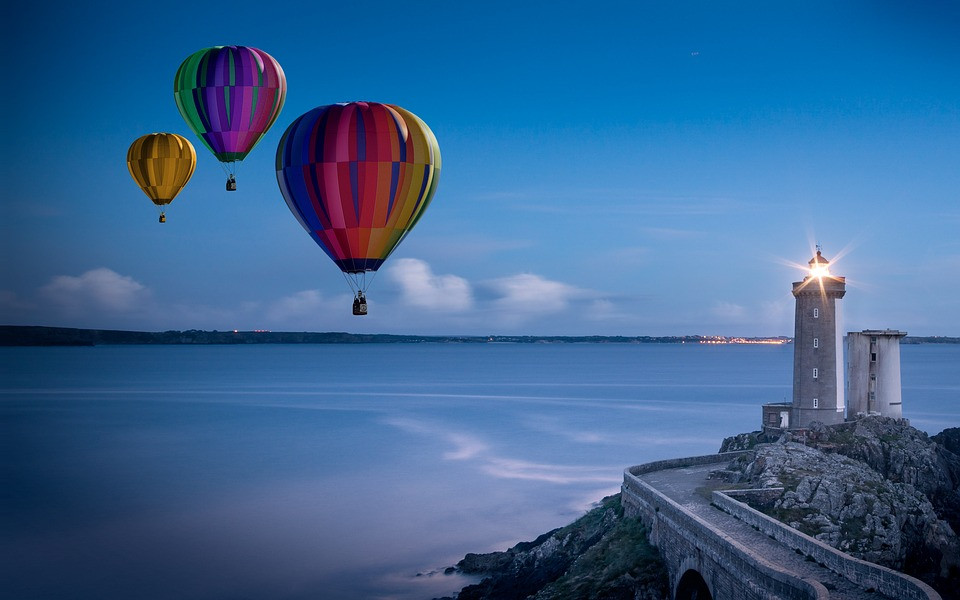
\includegraphics[width=7cm]{montgolfieres}};
    \def\x{10}
    \node (probas) at (\x+0.5, 2) {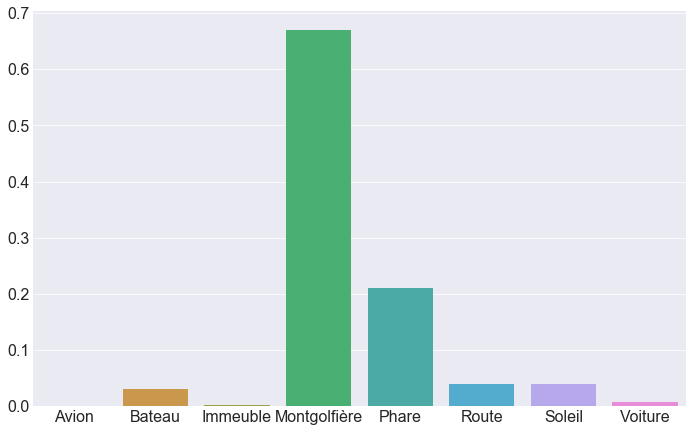
\includegraphics[width=6cm]{montgolfieres_probas}};
    \node (segmentation) at (\x-0.5, -2) {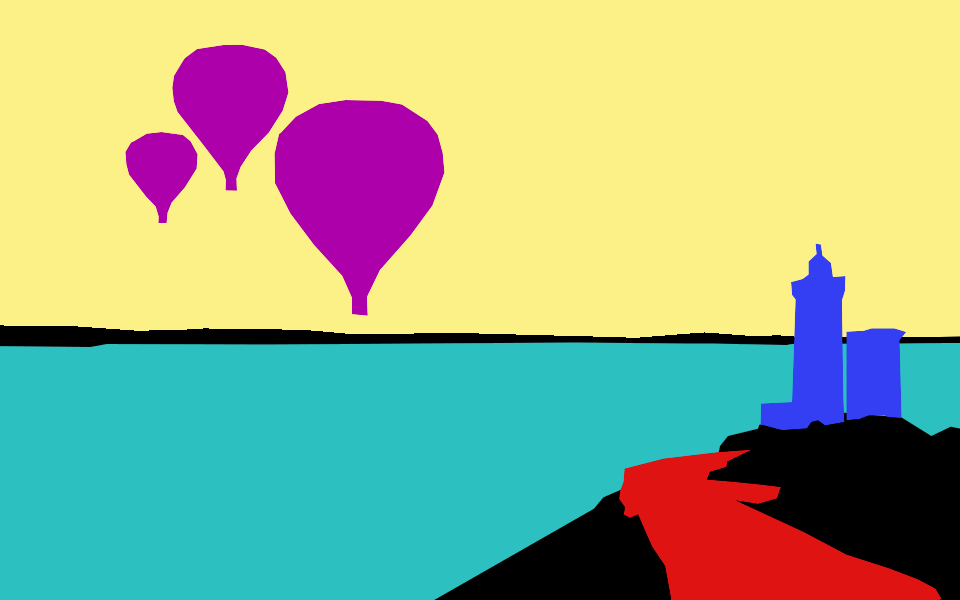
\includegraphics[width=3.8cm]{montgolfieres_segmentation}};
    \node [minimum width=2.1cm, fill=lpurple] at (\x+2.5, -1) {\footnotesize \textcolor{white}{Montgolfière}};
    \node [minimum width=2.1cm, fill=lyellow] at (\x+2.5, -1.5) {\footnotesize Ciel};
    \node [minimum width=2.1cm, fill=lcyan] at (\x+2.5, -2) {\footnotesize Eau};
    \node [minimum width=2.1cm, fill=lblue] at (\x+2.5, -2.5) {\footnotesize \textcolor{white}{Bâtiment}};
    \node [minimum width=2.1cm, fill=lred] at (\x+2.5, -3) {\footnotesize Route};
    \node[below] at (probas.south) {Classification};
    \node[below] at (segmentation.south) {Segmentation};
    \node[below] at (input.south) {Image};
    \draw (input) edge[in=180,out=0,->,ultra thick] (probas);
    \draw (input) edge[in=180,out=0,->,ultra thick] (segmentation);
  \end{tikzpicture}
\end{document}
}
  \caption{Exemple de classification et de segmentation sur une même image. La classification s'intéresse à la reconnaissance d'objet pour toute l'image, tandis que la segmentation opère sur chaque pixel.}
  \label{fig:classif_vs_seg}
\end{figure}

La segmentation d'image est une des premières tâches envisagée dans le cadre de la vision artificielle.
La légende veut que Minsky en 1964 ait demandé à un ses étudiants, Gerald Sussman, de \og passer l'été à connecter une caméra à un ordinateur et réussir à faire en sorte que l'ordinateur décrive ce qu'il voit \fg\footnote{``\emph{spend the summer linking a camera to a computer and getting the computer to describe what it saw}'', tel que rapporté par ~\citet{szeliski_computer_2011}, citant lui-même~\citet{boden_mind_2008} reprenant~\citet{crevier_ai_1993}.}.
La tâche envisagée par Minsky et Papert pour le \emph{Summer Vision Project} consistait notamment à \og construire un système de programmes divisant une image issue d'un tube dissecteur\footnote{En référence au \emph{vidisector}, le dissecteur d'images inventé par Philo Farnsworth en 1927 sur le principe du tube cathodique. L'appareil reçoit de la lumière, ce qui stimule une photocathode et émet des électrons, produisant un signal électrique permettant de représenter l'image. C'est l'inverse de l'écran de télévision.} en différentes régions telles que\,: plutôt des objets, plutôt l'arrière-plan, ou du chaos\fg{} avec pour objectif final \og l'identification d'objets, qui nommera chaque objet en les faisant correspondre avec un vocabulaire d'objets connus.\fg{}~\cite{papert_summer_1966}
Dès le départ, la reconnaissance de formes s'intéresse donc au découpage sémantique des images afin de comprendre les scènes visuelles qu'elles représentent.
Si cette tâche semble triviale pour un humain, elle est représente pourtant un défi considérable pour la machine et l'équipe de Minsky se heurte au paradoxe de Moravec~\cite{moravec_mind_1988}\,: \og il est relativement aisé de mettre des ordinateurs au niveau d'un humain adulte dans le cadre d'un test d'intelligence ou d'une partie de dames, mais difficile voire impossible de leur donner les capacités de perception et la mobilité d'un bébé\fg{}\footnote{\emph{``it is comparatively easy to make computers exhibit adult level performance on intelligence tests or playing checkers, and difficult or impossible to give them the skills of a one-year-old when it comes to perception and mobility''}}.

De nombreux travaux se sont dès lors penchés sur le problème de la reconnaissance d'objet, c'est-à-dire l'identification et le nommage d'un objet présent dans une image. On parlera ici de classification d'images, tâche consistant à associer une classe d'objet à une image. Cette tâche a concentré la majorité des efforts de la communauté, de l'utilisation de descripteurs \emph{ad hoc}~\cite{ullman_aligning_1989} aux caractéristiques apprises~\cite{vidal-naquet_object_2003} en passant par les modèles probabilistes~\cite{schneiderman_probabilistic_1998}. L'arrivée récente de larges bases de données d'images annotées comme CIFAR-10 et CIFAR-100~\cite{krizhevsky_learning_2009}, puis ImageNet~\cite{deng_imagenet_2009,russakovsky_imagenet_2015} ont notamment permis d'aboutir au succès des réseaux convolutifs profonds en classification de chiffres sur la base de données MNIST~\cite{lecun_gradient-based_1998}, en reconnaissance de panneaux de signalisation~\cite{stallkamp_german_2011}, en identification de caractères chinois~\cite{liu_icdar_2011} et bien sûr en reconnaissance d'objets en tout genre sur ImageNet~\cite{krizhevsky_imagenet_2012}.

\begin{figure}[t]
  \resizebox{\textwidth}{!}{
    \documentclass{standalone}
\usepackage[utf8]{inputenc}
\usepackage[T1]{fontenc}
\usepackage{tikz}
\usepackage{ifthen}
%%%%%%%%%%%%%%%%%%%%%%%%%%%%%%%%%%%%%%%%
%           Commandes perso            %
%%%%%%%%%%%%%%%%%%%%%%%%%%%%%%%%%%%%%%%%

%% Figures centrées, et en position 'here, top, bottom or page'
\newenvironment{figureth}{%
		\begin{figure}[htbp]
			\centering
	}{
		\end{figure}
		}


%% Tableaux centrés, et en position 'here, top, bottom or page'
\newenvironment{tableth}{%
		\begin{table}[htbp]
			\centering
			%\rowcolors{1}{coleurtableau}{coleurtableau}
	}{
		\end{table}
		}

%% Sous-figures centrées, en position 'top'
\newenvironment{subfigureth}[1]{%
	\begin{subfigure}[t]{#1}
	\centering
}{
	\end{subfigure}
}

\newcommand{\citationChap}[2]{%
	\epigraph{\og \textit{#1} \fg{}}{#2}
}

%% On commence par une page impaire quand on change le style de numérotation de pages
\let\oldpagenumbering\pagenumbering
\renewcommand{\pagenumbering}[1]{%
	\cleardoublepage
	\oldpagenumbering{#1}
}

%% Légende du dataset ISPRS
\newcommand\isprslegende{
Légende\,: \textcolor{Black}{blanc}\,: routes, \textcolor{Blue}{bleu}\,: bâtiments, \textcolor{Cerulean}{cyan}\,: végétation basse, \textcolor{OliveGreen}{vert}\,: arbres, \textcolor{Dandelion}{jaune}\,: véhicules, \textcolor{BrickRed}{rouge}\,: autre.
}

%% Dessiner des réseaux de neurones avec Tikz
\newcommand{\convlayer}[9]{%{h}{w}{d}{name}{color}{x}{y}{z}%{note w}{note h}{note d}
   \def\h{#1}
   \def\w{#2}
   \def\d{#3}
   \def\name{#4}
   \ifthenelse {\equal{#5} {}} {\def\col{white}} {\def\col{#5}}
   \def\x{#6}
   \ifthenelse {\equal{#7} {}} {\def\y{0}} {\def\y{#7}}
   \ifthenelse {\equal{#8} {}} {\def\z{0}} {\def\z{#8}}
   % ne faites pas ça chez vous !
   \ifthenelse {\equal{#9} {}} {\convlayercontinued{}{}{}} {\convlayercontinued#9}
}

\newcommand\convlayercontinued[3]{
   \def\notew{#1}
   \def\noteh{#2}
   \def\noted{#3}
   \coordinate (A) at (\x-\d/2,  \y-\h/2, \z-\w/2);
   \coordinate (B) at (\x-\d/2,  \y-\h/2, \z+\w/2);
   \coordinate (C) at (\x-\d/2,  \y+\h/2, \z+\w/2);
   \coordinate (D) at (\x-\d/2,  \y+\h/2, \z-\w/2);
   \coordinate (E) at (\x+\d/2,  \y-\h/2, \z-\w/2);
   \coordinate (F) at (\x+\d/2,  \y-\h/2, \z+\w/2);
   \coordinate (G) at (\x+\d/2,  \y+\h/2, \z+\w/2);
   \coordinate (H) at (\x+\d/2,  \y+\h/2, \z-\w/2);

    \draw [draw opacity=0.3, fill opacity=0.8, fill=\col!60!white] (A) -- (B) -- (C) -- (D) -- cycle;
    \draw [draw opacity=0.3, fill opacity=0.8, fill=\col!60!white] (A) -- (B) -- (F) -- (E) -- cycle;
    % Face haut
    %\draw [left color=\col!60!white, right color=\col!80!white, shading=axis, shading angle=180] (C) -- (D)  -- (H) -- (G) -- cycle;
    \draw [fill opacity=0.9, fill=\col!70!white] (C) -- node[rotate=45,above] {\small \name} (D) -- (H) -- (G) -- cycle;
    %\draw [fill opacity=0.9, fill=\col!70!white] (C) -- (D) -- node[above] {\small \name} (H) -- (G) -- cycle;
    % Face droite
    \draw [fill opacity=0.9, fill=\col!60!white] (E) -- node[pos=0.75,rotate=45,below] {\scriptsize \notew} (F) -- (G) --  (H) -- cycle;
    % Face avant
    %\draw [shading=axis, left color=\col!60!white, right color=\col!40!white, shading angle=-45] (B) -- node[above,rotate=90] {\scriptsize \noteh} (C) -- (G) -- (F) -- node[below] {\scriptsize \noted}  cycle;
    \draw [fill opacity=0.9, fill=\col!50!white] (B) -- node[above,rotate=90] {\scriptsize \noteh} (C) -- (G) -- (F) -- node[below] {\scriptsize \noted}  cycle;
}

\newcommand{\fclayer}[8]{%{h}{w}{name}{color}{x}{y}{z}
   \def\h{#1}
   \def\w{#2}
   \def\name{#3}
   \ifthenelse {\equal{#4} {}} {\def\col{white}} {\def\col{#4}}
   \def\x{#5}
   \def\y{#6}
   \def\z{#7}
   \def\note{#8}
   \coordinate (A) at (\x-\w/2,  \y-\h/2, \z);
   \coordinate (B) at (\x+\w/2,  \y-\h/2, \z);
   \coordinate (C) at (\x+\w/2,  \y+\h/2, \z);
   \coordinate (D) at (\x-\w/2,  \y+\h/2, \z);

   \pgfmathparse{4*\w}\let\boxwidth\pgfmathresult
    \draw [fill=\col] (A) -- node[below,text width=\boxwidth cm,align=center] {\scriptsize \note} (B) -- (C) -- (D) -- cycle;

    \node (N) at ($(A)!0.5!(B)+(0,-1,0)$) {\name};
}

\newcommand{\alexnet}[4]{%{scale}{x}{y}{z}
  \def\scale{#1}
  \def\alexx{#2}
  \def\alexy{#3}
  \def\alexz{#4}


  \def\coblue{blue!50!white}
  \def\fcgrey{gray!50!white}

  \convlayer{1.3*\scale}{1.3*\scale}{0.02*\scale}{Image}{\coblue}{\alexx}{\alexy}{\alexz}{{227}{227}{3}}
  \convlayer{1.1*\scale}{1.1*\scale}{0.08*\scale}{Conv1}{\coblue}{\alexx+0.7*\scale}{\alexy}{\alexz}{{55}{55}{96}}
  \convlayer{0.7*\scale}{0.7*\scale}{0.5*\scale}{Conv2}{\coblue}{\alexx+1.5*\scale}{\alexy}{\alexz}{{27}{27}{256}}
  \convlayer{0.5*\scale}{0.5*\scale}{0.8*\scale}{Conv3}{\coblue}{\alexx+2.6*\scale}{\alexy}{\alexz}{{13}{13}{384}}
  \convlayer{0.5*\scale}{0.5*\scale}{0.8*\scale}{Conv4}{\coblue}{\alexx+3.8*\scale}{\alexy}{\alexz}{{13}{13}{384}}
  \convlayer{0.5*\scale}{0.5*\scale}{0.5*\scale}{Conv5}{\coblue}{\alexx+4.8*\scale}{\alexy}{\alexz}{{13}{13}{256}}
  \fclayer{\scale}{0.1*\scale}{FC1}{\fcgrey}{\alexx+5.4*\scale}{\alexy}{\alexz}{4096}
  \fclayer{\scale}{0.1*\scale}{FC2}{\fcgrey}{\alexx+5.7*\scale}{\alexy}{\alexz}{4096}
  \fclayer{\scale}{0.1*\scale}{FC3}{\fcgrey}{\alexx+6.0*\scale}{\alexy}{\alexz}{1000}
}

\newcommand{\imagelayer}[7]{%{width}{x}{y}{z}{path}{text_up}{text_down}
    \pgfmathparse{#1}\let\w\pgfmathresult
    \begin{scope}[canvas is yz plane at x=#2]
     \node[transform shape] (source) at (#3, #4) {\includegraphics[angle=-90,width=\w cm]{#5}};
    \end{scope}
     \node [transform shape, rotate=45, above] at (source.east) {#6};
     \node [transform shape, rotate=45, below] at (source.west) {\scriptsize{#7}};
}

\def\fourier{\mathcal{F}}

\newcommand{\lightspectrum}{%
\pgfplotsset{
    % this *defines* a custom colormap ...
    colormap={slategraywhite}{color(0cm)=(red); color(1cm)=(red); color(2cm)=(red); color(3cm)=(red); color(4cm)=(orange); color(5cm)=(yellow); color(6cm)=(green); color(7cm)=(blue); color(8cm)=(blue); color(9cm)=(purple); color(10cm)=(purple); color(12cm)=(black)}
}
\node at (1.5, 2.7) {\small 1mm};
\node at (4, 3) {Infrarouge};
\node at (7.75, 2.7) {\small 800nm};
\node at (9, 3) {Visible};
\node at (10.5, 2.7) {\small 400nm};
\node at (12, 3) {Ultraviolet};
\node at (13.5, 2.7) {\small 10nm};
\draw[->] (1, 2.5) -- (14, 2.5);
\begin{axis}[hide axis,width=16cm,height=4cm,colormap name=slategraywhite]
\addplot[domain=20:1000,samples=1500,ultra thick, point meta=x*x,mesh]{sin(x*x/80)};
\end{axis}
}

% Union généralisée
\newcommand{\wbigcup}{\mathop{\bigcup}\displaylimits}

\newcommand{\res}[2]{#1 {\footnotesize $\pm$ #2}}
\newcommand{\bres}[2]{\textbf{#1} {\footnotesize $\pm$ #2}}
\newcommand{\bbres}[2]{\res{\textit{#1}}{#2}}

\newcommand{\drawkernel}[9]{
\begin{tikzpicture}
	\draw[step=1cm,gray!50!white,very thin] (0,0) grid (3,3);
	\kernelnode{0.5}{0.5}{#1};
	\kernelnode{0.5}{1.5}{#2};
	\kernelnode{0.5}{2.5}{#3};
	\kernelnode{1.5}{0.5}{#4};
	\kernelnode{1.5}{1.5}{#5};
	\kernelnode{1.5}{2.5}{#6};
	\kernelnode{2.5}{0.5}{#7};
	\kernelnode{2.5}{1.5}{#8};
	\kernelnode{2.5}{2.5}{#9};
\end{tikzpicture}
}

\newcommand{\kernelnode}[3]{%{x}{y}{value}
	\ifthenelse{\equal{#3}{0}}{
		\def\kcolor{gray}
	}{
		\def\kcolor{black}
	}
	\node[\kcolor] at (#1, #2) {#3};
}

\newcommand{\chapsummary}[1]{
\section*{Résumé du chapitre :}
\parbox{0.9\linewidth}{
\setlength{\parindent}{4ex}
#1}
}

\newcommand{\eqname}[1]{\tag*{\small (#1)}}


\begin{document}
  \begin{tikzpicture}
  \usetikzlibrary{calc}
  \usetikzlibrary{3d}

  \def\scale{3}
  \def\netx{0}
  \def\nety{0}
  \def\netz{0}

  \def\coblue{blue!50!gray}
  \def\coorange{orange!50!gray}
  \def\cogreen{green!50!gray}
  \def\copurple{purple!50!white}

  \imagelayer{1.3*\scale}{0.05*\scale+\netx}{\nety}{\netz}{nobu_gray}{Image}{$32\times32\times1$}
  \convlayer{1.1*\scale}{1.1*\scale}{0.1*\scale}{Conv1}{\coblue}{\netx+0.8*\scale}{\nety}{\netz}{{28}{28}{6}}
  \convlayer{0.7*\scale}{0.7*\scale}{0.1*\scale}{Pool1}{\coorange}{\netx+1.5*\scale}{\nety}{\netz}{{14}{14}{6}}
  \convlayer{0.7*\scale}{0.7*\scale}{0.4*\scale}{Conv2}{\coblue}{\netx+2.4*\scale}{\nety}{\netz}{{10}{10}{16}}
  \convlayer{0.5*\scale}{0.5*\scale}{0.1*\scale}{Pool2}{\coorange}{\netx+3.3*\scale}{\nety}{\netz}{{5}{5}{16}}
  \fclayer{\scale}{0.1*\scale}{FC1}{\copurple}{\netx+3.9*\scale}{\nety}{\netz}{120}
  \fclayer{\scale}{0.1*\scale}{FC2}{\copurple}{\netx+4.3*\scale}{\nety}{\netz}{80}
  \fclayer{0.8*\scale}{0.1*\scale}{FC3}{\copurple}{\netx+4.7*\scale}{\nety}{\netz}{10}
  \node (out) at (\netx+5.8*\scale,\nety) {\Large ``Chat''};
  \draw[->] (\netx+4.75*\scale,\nety) -- (out.west);

  \end{tikzpicture}
\end{document}

  }
  \caption{Architecture LeNet-5~\cite{lecun_gradient-based_1998}}
  \label{fig:lenet}
\end{figure}

L'architecture LeNet-5, developpée par \citet{lecun_gradient-based_1998}, a posé les bases des \gls{CNN}. Elle consiste en deux couches convolutives suivies de trois couches entièrement connectées, comme illustré dans la~\cref{fig:lenet}. La partie convolutive du modèle réalise l'extraction de caractéristiques dans le domaine image, tandis que les couches entièrement connectées opèrent sur une représentation vectorielle unidimensionnelle et réalisent la classification finale. Initialement, LeNet-5 a été développé pour la reconnaissance de chiffres manuscrits dans des images en niveaux de gris et est conçu pour des images de dimensions $32\times32$px. En comparaison de la taille de l'image, les filtres convolutifs utilisés sont relativement grands puisque les noyaux de convolution sont de taille $5\times5$. La première couche $C1$ comporte 6 noyaux, c'est-à-dire que six cartes d'activation sont générées. Elles sont sous-échantillonnées avec un pas de 2, puis transmises à la couche convolutive suivante $C2$. Chaque carte d'activation de $C1$ est filtrée par chaque noyau de convolution de la couche $C2$, qui en comporte 16. Les cartes sont à nouveau sous-échantillonnée, ce qui produit finalement 16 cartes d'activation $5\times5$. Celles-ci sont alors aplaties en un vecteur de taille $1\times400$, entièrement connecté à une première couche cachée de dimension $120$, puis à une seconde de dimension $84$. Finalement, ce descripteur est entièrement connecté au vecteur de taille $10$, chaque activation correspondant alors à un des 10 chiffres possibles. La présence des couches entièrement connectées, dont le nombre de neurones est fixé, impose aux cartes d'activation issues des couches convolutives d'être de la bonne dimension. Cette contrainte impose en cascade que la taille des images traitées par LeNet soit toujours la même. Utiliser des images d'autres dimensions nécessiterait de ré-entraîner des couches entièrement connectées avec le nombre adéquat de neurones. Cette déficience due à la présence des couches entièrement connectées est partagée par la plupart des \gls{CNN}.

\begin{figure}[t]
  \resizebox{\textwidth}{!}{
    \documentclass{standalone}
\usepackage[utf8]{inputenc}
\usepackage[T1]{fontenc}
\usepackage{tikz}
\usepackage{ifthen}
%%%%%%%%%%%%%%%%%%%%%%%%%%%%%%%%%%%%%%%%
%           Commandes perso            %
%%%%%%%%%%%%%%%%%%%%%%%%%%%%%%%%%%%%%%%%

%% Figures centrées, et en position 'here, top, bottom or page'
\newenvironment{figureth}{%
		\begin{figure}[htbp]
			\centering
	}{
		\end{figure}
		}


%% Tableaux centrés, et en position 'here, top, bottom or page'
\newenvironment{tableth}{%
		\begin{table}[htbp]
			\centering
			%\rowcolors{1}{coleurtableau}{coleurtableau}
	}{
		\end{table}
		}

%% Sous-figures centrées, en position 'top'
\newenvironment{subfigureth}[1]{%
	\begin{subfigure}[t]{#1}
	\centering
}{
	\end{subfigure}
}

\newcommand{\citationChap}[2]{%
	\epigraph{\og \textit{#1} \fg{}}{#2}
}

%% On commence par une page impaire quand on change le style de numérotation de pages
\let\oldpagenumbering\pagenumbering
\renewcommand{\pagenumbering}[1]{%
	\cleardoublepage
	\oldpagenumbering{#1}
}

%% Légende du dataset ISPRS
\newcommand\isprslegende{
Légende\,: \textcolor{Black}{blanc}\,: routes, \textcolor{Blue}{bleu}\,: bâtiments, \textcolor{Cerulean}{cyan}\,: végétation basse, \textcolor{OliveGreen}{vert}\,: arbres, \textcolor{Dandelion}{jaune}\,: véhicules, \textcolor{BrickRed}{rouge}\,: autre.
}

%% Dessiner des réseaux de neurones avec Tikz
\newcommand{\convlayer}[9]{%{h}{w}{d}{name}{color}{x}{y}{z}%{note w}{note h}{note d}
   \def\h{#1}
   \def\w{#2}
   \def\d{#3}
   \def\name{#4}
   \ifthenelse {\equal{#5} {}} {\def\col{white}} {\def\col{#5}}
   \def\x{#6}
   \ifthenelse {\equal{#7} {}} {\def\y{0}} {\def\y{#7}}
   \ifthenelse {\equal{#8} {}} {\def\z{0}} {\def\z{#8}}
   % ne faites pas ça chez vous !
   \ifthenelse {\equal{#9} {}} {\convlayercontinued{}{}{}} {\convlayercontinued#9}
}

\newcommand\convlayercontinued[3]{
   \def\notew{#1}
   \def\noteh{#2}
   \def\noted{#3}
   \coordinate (A) at (\x-\d/2,  \y-\h/2, \z-\w/2);
   \coordinate (B) at (\x-\d/2,  \y-\h/2, \z+\w/2);
   \coordinate (C) at (\x-\d/2,  \y+\h/2, \z+\w/2);
   \coordinate (D) at (\x-\d/2,  \y+\h/2, \z-\w/2);
   \coordinate (E) at (\x+\d/2,  \y-\h/2, \z-\w/2);
   \coordinate (F) at (\x+\d/2,  \y-\h/2, \z+\w/2);
   \coordinate (G) at (\x+\d/2,  \y+\h/2, \z+\w/2);
   \coordinate (H) at (\x+\d/2,  \y+\h/2, \z-\w/2);

    \draw [draw opacity=0.3, fill opacity=0.8, fill=\col!60!white] (A) -- (B) -- (C) -- (D) -- cycle;
    \draw [draw opacity=0.3, fill opacity=0.8, fill=\col!60!white] (A) -- (B) -- (F) -- (E) -- cycle;
    % Face haut
    %\draw [left color=\col!60!white, right color=\col!80!white, shading=axis, shading angle=180] (C) -- (D)  -- (H) -- (G) -- cycle;
    \draw [fill opacity=0.9, fill=\col!70!white] (C) -- node[rotate=45,above] {\small \name} (D) -- (H) -- (G) -- cycle;
    %\draw [fill opacity=0.9, fill=\col!70!white] (C) -- (D) -- node[above] {\small \name} (H) -- (G) -- cycle;
    % Face droite
    \draw [fill opacity=0.9, fill=\col!60!white] (E) -- node[pos=0.75,rotate=45,below] {\scriptsize \notew} (F) -- (G) --  (H) -- cycle;
    % Face avant
    %\draw [shading=axis, left color=\col!60!white, right color=\col!40!white, shading angle=-45] (B) -- node[above,rotate=90] {\scriptsize \noteh} (C) -- (G) -- (F) -- node[below] {\scriptsize \noted}  cycle;
    \draw [fill opacity=0.9, fill=\col!50!white] (B) -- node[above,rotate=90] {\scriptsize \noteh} (C) -- (G) -- (F) -- node[below] {\scriptsize \noted}  cycle;
}

\newcommand{\fclayer}[8]{%{h}{w}{name}{color}{x}{y}{z}
   \def\h{#1}
   \def\w{#2}
   \def\name{#3}
   \ifthenelse {\equal{#4} {}} {\def\col{white}} {\def\col{#4}}
   \def\x{#5}
   \def\y{#6}
   \def\z{#7}
   \def\note{#8}
   \coordinate (A) at (\x-\w/2,  \y-\h/2, \z);
   \coordinate (B) at (\x+\w/2,  \y-\h/2, \z);
   \coordinate (C) at (\x+\w/2,  \y+\h/2, \z);
   \coordinate (D) at (\x-\w/2,  \y+\h/2, \z);

   \pgfmathparse{4*\w}\let\boxwidth\pgfmathresult
    \draw [fill=\col] (A) -- node[below,text width=\boxwidth cm,align=center] {\scriptsize \note} (B) -- (C) -- (D) -- cycle;

    \node (N) at ($(A)!0.5!(B)+(0,-1,0)$) {\name};
}

\newcommand{\alexnet}[4]{%{scale}{x}{y}{z}
  \def\scale{#1}
  \def\alexx{#2}
  \def\alexy{#3}
  \def\alexz{#4}


  \def\coblue{blue!50!white}
  \def\fcgrey{gray!50!white}

  \convlayer{1.3*\scale}{1.3*\scale}{0.02*\scale}{Image}{\coblue}{\alexx}{\alexy}{\alexz}{{227}{227}{3}}
  \convlayer{1.1*\scale}{1.1*\scale}{0.08*\scale}{Conv1}{\coblue}{\alexx+0.7*\scale}{\alexy}{\alexz}{{55}{55}{96}}
  \convlayer{0.7*\scale}{0.7*\scale}{0.5*\scale}{Conv2}{\coblue}{\alexx+1.5*\scale}{\alexy}{\alexz}{{27}{27}{256}}
  \convlayer{0.5*\scale}{0.5*\scale}{0.8*\scale}{Conv3}{\coblue}{\alexx+2.6*\scale}{\alexy}{\alexz}{{13}{13}{384}}
  \convlayer{0.5*\scale}{0.5*\scale}{0.8*\scale}{Conv4}{\coblue}{\alexx+3.8*\scale}{\alexy}{\alexz}{{13}{13}{384}}
  \convlayer{0.5*\scale}{0.5*\scale}{0.5*\scale}{Conv5}{\coblue}{\alexx+4.8*\scale}{\alexy}{\alexz}{{13}{13}{256}}
  \fclayer{\scale}{0.1*\scale}{FC1}{\fcgrey}{\alexx+5.4*\scale}{\alexy}{\alexz}{4096}
  \fclayer{\scale}{0.1*\scale}{FC2}{\fcgrey}{\alexx+5.7*\scale}{\alexy}{\alexz}{4096}
  \fclayer{\scale}{0.1*\scale}{FC3}{\fcgrey}{\alexx+6.0*\scale}{\alexy}{\alexz}{1000}
}

\newcommand{\imagelayer}[7]{%{width}{x}{y}{z}{path}{text_up}{text_down}
    \pgfmathparse{#1}\let\w\pgfmathresult
    \begin{scope}[canvas is yz plane at x=#2]
     \node[transform shape] (source) at (#3, #4) {\includegraphics[angle=-90,width=\w cm]{#5}};
    \end{scope}
     \node [transform shape, rotate=45, above] at (source.east) {#6};
     \node [transform shape, rotate=45, below] at (source.west) {\scriptsize{#7}};
}

\def\fourier{\mathcal{F}}

\newcommand{\lightspectrum}{%
\pgfplotsset{
    % this *defines* a custom colormap ...
    colormap={slategraywhite}{color(0cm)=(red); color(1cm)=(red); color(2cm)=(red); color(3cm)=(red); color(4cm)=(orange); color(5cm)=(yellow); color(6cm)=(green); color(7cm)=(blue); color(8cm)=(blue); color(9cm)=(purple); color(10cm)=(purple); color(12cm)=(black)}
}
\node at (1.5, 2.7) {\small 1mm};
\node at (4, 3) {Infrarouge};
\node at (7.75, 2.7) {\small 800nm};
\node at (9, 3) {Visible};
\node at (10.5, 2.7) {\small 400nm};
\node at (12, 3) {Ultraviolet};
\node at (13.5, 2.7) {\small 10nm};
\draw[->] (1, 2.5) -- (14, 2.5);
\begin{axis}[hide axis,width=16cm,height=4cm,colormap name=slategraywhite]
\addplot[domain=20:1000,samples=1500,ultra thick, point meta=x*x,mesh]{sin(x*x/80)};
\end{axis}
}

% Union généralisée
\newcommand{\wbigcup}{\mathop{\bigcup}\displaylimits}

\newcommand{\res}[2]{#1 {\footnotesize $\pm$ #2}}
\newcommand{\bres}[2]{\textbf{#1} {\footnotesize $\pm$ #2}}
\newcommand{\bbres}[2]{\res{\textit{#1}}{#2}}

\newcommand{\drawkernel}[9]{
\begin{tikzpicture}
	\draw[step=1cm,gray!50!white,very thin] (0,0) grid (3,3);
	\kernelnode{0.5}{0.5}{#1};
	\kernelnode{0.5}{1.5}{#2};
	\kernelnode{0.5}{2.5}{#3};
	\kernelnode{1.5}{0.5}{#4};
	\kernelnode{1.5}{1.5}{#5};
	\kernelnode{1.5}{2.5}{#6};
	\kernelnode{2.5}{0.5}{#7};
	\kernelnode{2.5}{1.5}{#8};
	\kernelnode{2.5}{2.5}{#9};
\end{tikzpicture}
}

\newcommand{\kernelnode}[3]{%{x}{y}{value}
	\ifthenelse{\equal{#3}{0}}{
		\def\kcolor{gray}
	}{
		\def\kcolor{black}
	}
	\node[\kcolor] at (#1, #2) {#3};
}

\newcommand{\chapsummary}[1]{
\section*{Résumé du chapitre :}
\parbox{0.9\linewidth}{
\setlength{\parindent}{4ex}
#1}
}

\newcommand{\eqname}[1]{\tag*{\small (#1)}}


\begin{document}
  \begin{tikzpicture}
  \usetikzlibrary{calc}
  \usetikzlibrary{3d}

  \def\scale{4}
  \def\alexx{0}
  \def\alexy{0}
  \def\alexz{0}

  \def\coblue{blue!50!gray}
  \def\coorange{orange!50!gray}
  \def\cogreen{green!50!gray}
  \def\copurple{purple!50!white}

  \imagelayer{1.3*\scale}{0.*\scale+\alexx}{\alexy}{\alexz}{nobu}{Image}{$224\times224\times3$}
  \convlayer{1.1*\scale}{1.1*\scale}{0.1*\scale}{Conv1}{\coblue}{\alexx+0.6*\scale}{\alexy}{\alexz}{{55}{55}{96}}
  \convlayer{0.7*\scale}{0.7*\scale}{0.1*\scale}{Pool1}{\coorange}{\alexx+1*\scale}{\alexy}{\alexz}{{}{}{96}}
  \convlayer{0.7*\scale}{0.7*\scale}{0.1*\scale}{LRN}{\cogreen}{\alexx+1.35*\scale}{\alexy}{\alexz}{{}{}{96}}
  \convlayer{0.7*\scale}{0.7*\scale}{0.4*\scale}{Conv2}{\coblue}{\alexx+2*\scale}{\alexy}{\alexz}{{27}{27}{256}}
  \convlayer{0.5*\scale}{0.5*\scale}{0.1*\scale}{Pool2}{\coorange}{\alexx+2.5*\scale}{\alexy}{\alexz}{{13}{13}{}}
  \convlayer{0.5*\scale}{0.5*\scale}{0.1*\scale}{LRN}{\cogreen}{\alexx+2.75*\scale}{\alexy}{\alexz}{{}{}{}}
  \convlayer{0.5*\scale}{0.5*\scale}{0.6*\scale}{Conv3}{\coblue}{\alexx+3.35*\scale}{\alexy}{\alexz}{{}{}{384}}
  \convlayer{0.5*\scale}{0.5*\scale}{0.6*\scale}{Conv4}{\coblue}{\alexx+4.2*\scale}{\alexy}{\alexz}{{}{}{384}}
  \convlayer{0.5*\scale}{0.5*\scale}{0.4*\scale}{Conv5}{\coblue}{\alexx+5*\scale}{\alexy}{\alexz}{{}{}{256}}
  \convlayer{0.3*\scale}{0.3*\scale}{0.1*\scale}{Pool5}{\coorange}{\alexx+5.5*\scale}{\alexy}{\alexz}{{7}{7}{256}}
  \fclayer{\scale}{0.1*\scale}{FC1}{\copurple}{\alexx+5.8*\scale}{\alexy}{\alexz}{4096}
  \fclayer{\scale}{0.1*\scale}{FC2}{\copurple}{\alexx+6.05*\scale}{\alexy}{\alexz}{4096}
  \fclayer{0.8*\scale}{0.1*\scale}{FC3}{\copurple}{\alexx+6.3*\scale}{\alexy}{\alexz}{1000}
  \node (out) at (\alexx+6.7*\scale,\alexy) {\Large ``Chat''};
  \draw[->] (\alexx+6.35*\scale,\alexy) -- (out.west);

  \end{tikzpicture}
\end{document}

  }
  \caption{Architecture AlexNet~\cite{krizhevsky_imagenet_2012}}
  \label{fig:alexnet}
\end{figure}

Pour le traitement des images en couleur, le réseau AlexNet~\cite{krizhevsky_imagenet_2012} utilise une approche similaire. Ce modèle, détaillé dans la~\cref{fig:alexnet} comporte 8 couches, dont 5 convolutives, et traite des images \gls{RVB} de dimensions $224\times224$. La première convolution possède un noyau relativement grand, de dimensions $11\times11$ suivi d'un sous-échantillonnage, ce qui réduit fortement les dimensions de l'image. Ainsi, les cartes d'activation en sortie de la première couche sont de dimensions $96\times27\times27$, puis $256\times13\times13$ après la seconde. Une normalisation \gls{LRN} est utilisée après les deux premières convolutions pour favoriser la généralisation du modèle. La structure convolutive d'AlexNet est conçue de telle sorte à ce que le nombre de cartes d'activation augmente de façon inversement proportionnelle à la réduction des dimensions spatiales. Cela permet de conserver un nombre raisonnable de valeurs à calculer tout en accroissant l'expressivité de la représentation apprise. Les trois couches de convolutions suivantes sont suivies par un sous-échantillonnage final qui permet d'obtenir 256 cartes de dimensions $6\times6$, transformée en un vecteur de caractéristique de longueur $9216$. Les couches entièrement connectées le réduisent ensuite à 2048 puis le projettent dans un vecteur de classification de taille 1000, correspondant aux classes d'ImageNet~\cite{deng_imagenet_2009}. Ce modèle a permis à~\citet{krizhevsky_imagenet_2012} de remporter la compétition \gls{ILSVRC}~\cite{russakovsky_imagenet_2015} en 2012 avec un taux d'erreur de 15,3\%.

\citet{zeiler_visualizing_2014-1} se sont penchés sur l'architecture AlexNet afin d'établir un diagnostic de ses points forts et de ses points faibles. En particulier, ils proposent d'inverser les opérations de convolution afin de pouvoir relier les représentations internes aux pixels de l'image originale. Ils définissent ainsi les opérations transposées de la couche de convolution et du sous-échantillonnage et construisent un \emph{Deconvnet} permettant de visualiser les caractéristiques apprises par AlexNet. En outre, ils étudient attentivement les filtres convolutifs appris par les couches basses du réseau. Leurs travaux mettent en évidence plusieurs propriétés intéressantes. La première est que les caractéristiques des couches supérieures présentent une plus grande invariance aux transformations géométriques et colorimétriques de bas niveau, traduisant ainsi un meilleur niveau d'abstraction. La seconde est que les deux premières couches convolutives d'AlexNet contienennt des filtres liés aux hautes et basses fréquences, mais conservent peu d'information des fréquences intermédiaires. Ils proposent ainsi de remplacer la première couche, dont les noyaux sont de dimension $11\times11$, par des filtres $7\times7$ appliqués sur l'image avec un pas de 2 plutôt qu'un pas de 4, afin de conserver plus d'information. Leurs filtres appris de cette façon présentent une meilleure variété et moins de filtres ``morts'' à très faible amplitude. Enfin, la visualisation des représentations internes permet de constater que celles-ci ne sont pas aléatoires, mais possèdent bien une sémantique liée à la discrimination des objets, certains neurones se focalisant par exemple sur les visages, d'autres sur les roues, etc.

\begin{figure}[t]
  \resizebox{\textwidth}{!}{
    \documentclass{standalone}
\usepackage[utf8]{inputenc}
\usepackage[T1]{fontenc}
\usepackage{tikz}
\usepackage{ifthen}
%%%%%%%%%%%%%%%%%%%%%%%%%%%%%%%%%%%%%%%%
%           Commandes perso            %
%%%%%%%%%%%%%%%%%%%%%%%%%%%%%%%%%%%%%%%%

%% Figures centrées, et en position 'here, top, bottom or page'
\newenvironment{figureth}{%
		\begin{figure}[htbp]
			\centering
	}{
		\end{figure}
		}


%% Tableaux centrés, et en position 'here, top, bottom or page'
\newenvironment{tableth}{%
		\begin{table}[htbp]
			\centering
			%\rowcolors{1}{coleurtableau}{coleurtableau}
	}{
		\end{table}
		}

%% Sous-figures centrées, en position 'top'
\newenvironment{subfigureth}[1]{%
	\begin{subfigure}[t]{#1}
	\centering
}{
	\end{subfigure}
}

\newcommand{\citationChap}[2]{%
	\epigraph{\og \textit{#1} \fg{}}{#2}
}

%% On commence par une page impaire quand on change le style de numérotation de pages
\let\oldpagenumbering\pagenumbering
\renewcommand{\pagenumbering}[1]{%
	\cleardoublepage
	\oldpagenumbering{#1}
}

%% Légende du dataset ISPRS
\newcommand\isprslegende{
Légende\,: \textcolor{Black}{blanc}\,: routes, \textcolor{Blue}{bleu}\,: bâtiments, \textcolor{Cerulean}{cyan}\,: végétation basse, \textcolor{OliveGreen}{vert}\,: arbres, \textcolor{Dandelion}{jaune}\,: véhicules, \textcolor{BrickRed}{rouge}\,: autre.
}

%% Dessiner des réseaux de neurones avec Tikz
\newcommand{\convlayer}[9]{%{h}{w}{d}{name}{color}{x}{y}{z}%{note w}{note h}{note d}
   \def\h{#1}
   \def\w{#2}
   \def\d{#3}
   \def\name{#4}
   \ifthenelse {\equal{#5} {}} {\def\col{white}} {\def\col{#5}}
   \def\x{#6}
   \ifthenelse {\equal{#7} {}} {\def\y{0}} {\def\y{#7}}
   \ifthenelse {\equal{#8} {}} {\def\z{0}} {\def\z{#8}}
   % ne faites pas ça chez vous !
   \ifthenelse {\equal{#9} {}} {\convlayercontinued{}{}{}} {\convlayercontinued#9}
}

\newcommand\convlayercontinued[3]{
   \def\notew{#1}
   \def\noteh{#2}
   \def\noted{#3}
   \coordinate (A) at (\x-\d/2,  \y-\h/2, \z-\w/2);
   \coordinate (B) at (\x-\d/2,  \y-\h/2, \z+\w/2);
   \coordinate (C) at (\x-\d/2,  \y+\h/2, \z+\w/2);
   \coordinate (D) at (\x-\d/2,  \y+\h/2, \z-\w/2);
   \coordinate (E) at (\x+\d/2,  \y-\h/2, \z-\w/2);
   \coordinate (F) at (\x+\d/2,  \y-\h/2, \z+\w/2);
   \coordinate (G) at (\x+\d/2,  \y+\h/2, \z+\w/2);
   \coordinate (H) at (\x+\d/2,  \y+\h/2, \z-\w/2);

    \draw [draw opacity=0.3, fill opacity=0.8, fill=\col!60!white] (A) -- (B) -- (C) -- (D) -- cycle;
    \draw [draw opacity=0.3, fill opacity=0.8, fill=\col!60!white] (A) -- (B) -- (F) -- (E) -- cycle;
    % Face haut
    %\draw [left color=\col!60!white, right color=\col!80!white, shading=axis, shading angle=180] (C) -- (D)  -- (H) -- (G) -- cycle;
    \draw [fill opacity=0.9, fill=\col!70!white] (C) -- node[rotate=45,above] {\small \name} (D) -- (H) -- (G) -- cycle;
    %\draw [fill opacity=0.9, fill=\col!70!white] (C) -- (D) -- node[above] {\small \name} (H) -- (G) -- cycle;
    % Face droite
    \draw [fill opacity=0.9, fill=\col!60!white] (E) -- node[pos=0.75,rotate=45,below] {\scriptsize \notew} (F) -- (G) --  (H) -- cycle;
    % Face avant
    %\draw [shading=axis, left color=\col!60!white, right color=\col!40!white, shading angle=-45] (B) -- node[above,rotate=90] {\scriptsize \noteh} (C) -- (G) -- (F) -- node[below] {\scriptsize \noted}  cycle;
    \draw [fill opacity=0.9, fill=\col!50!white] (B) -- node[above,rotate=90] {\scriptsize \noteh} (C) -- (G) -- (F) -- node[below] {\scriptsize \noted}  cycle;
}

\newcommand{\fclayer}[8]{%{h}{w}{name}{color}{x}{y}{z}
   \def\h{#1}
   \def\w{#2}
   \def\name{#3}
   \ifthenelse {\equal{#4} {}} {\def\col{white}} {\def\col{#4}}
   \def\x{#5}
   \def\y{#6}
   \def\z{#7}
   \def\note{#8}
   \coordinate (A) at (\x-\w/2,  \y-\h/2, \z);
   \coordinate (B) at (\x+\w/2,  \y-\h/2, \z);
   \coordinate (C) at (\x+\w/2,  \y+\h/2, \z);
   \coordinate (D) at (\x-\w/2,  \y+\h/2, \z);

   \pgfmathparse{4*\w}\let\boxwidth\pgfmathresult
    \draw [fill=\col] (A) -- node[below,text width=\boxwidth cm,align=center] {\scriptsize \note} (B) -- (C) -- (D) -- cycle;

    \node (N) at ($(A)!0.5!(B)+(0,-1,0)$) {\name};
}

\newcommand{\alexnet}[4]{%{scale}{x}{y}{z}
  \def\scale{#1}
  \def\alexx{#2}
  \def\alexy{#3}
  \def\alexz{#4}


  \def\coblue{blue!50!white}
  \def\fcgrey{gray!50!white}

  \convlayer{1.3*\scale}{1.3*\scale}{0.02*\scale}{Image}{\coblue}{\alexx}{\alexy}{\alexz}{{227}{227}{3}}
  \convlayer{1.1*\scale}{1.1*\scale}{0.08*\scale}{Conv1}{\coblue}{\alexx+0.7*\scale}{\alexy}{\alexz}{{55}{55}{96}}
  \convlayer{0.7*\scale}{0.7*\scale}{0.5*\scale}{Conv2}{\coblue}{\alexx+1.5*\scale}{\alexy}{\alexz}{{27}{27}{256}}
  \convlayer{0.5*\scale}{0.5*\scale}{0.8*\scale}{Conv3}{\coblue}{\alexx+2.6*\scale}{\alexy}{\alexz}{{13}{13}{384}}
  \convlayer{0.5*\scale}{0.5*\scale}{0.8*\scale}{Conv4}{\coblue}{\alexx+3.8*\scale}{\alexy}{\alexz}{{13}{13}{384}}
  \convlayer{0.5*\scale}{0.5*\scale}{0.5*\scale}{Conv5}{\coblue}{\alexx+4.8*\scale}{\alexy}{\alexz}{{13}{13}{256}}
  \fclayer{\scale}{0.1*\scale}{FC1}{\fcgrey}{\alexx+5.4*\scale}{\alexy}{\alexz}{4096}
  \fclayer{\scale}{0.1*\scale}{FC2}{\fcgrey}{\alexx+5.7*\scale}{\alexy}{\alexz}{4096}
  \fclayer{\scale}{0.1*\scale}{FC3}{\fcgrey}{\alexx+6.0*\scale}{\alexy}{\alexz}{1000}
}

\newcommand{\imagelayer}[7]{%{width}{x}{y}{z}{path}{text_up}{text_down}
    \pgfmathparse{#1}\let\w\pgfmathresult
    \begin{scope}[canvas is yz plane at x=#2]
     \node[transform shape] (source) at (#3, #4) {\includegraphics[angle=-90,width=\w cm]{#5}};
    \end{scope}
     \node [transform shape, rotate=45, above] at (source.east) {#6};
     \node [transform shape, rotate=45, below] at (source.west) {\scriptsize{#7}};
}

\def\fourier{\mathcal{F}}

\newcommand{\lightspectrum}{%
\pgfplotsset{
    % this *defines* a custom colormap ...
    colormap={slategraywhite}{color(0cm)=(red); color(1cm)=(red); color(2cm)=(red); color(3cm)=(red); color(4cm)=(orange); color(5cm)=(yellow); color(6cm)=(green); color(7cm)=(blue); color(8cm)=(blue); color(9cm)=(purple); color(10cm)=(purple); color(12cm)=(black)}
}
\node at (1.5, 2.7) {\small 1mm};
\node at (4, 3) {Infrarouge};
\node at (7.75, 2.7) {\small 800nm};
\node at (9, 3) {Visible};
\node at (10.5, 2.7) {\small 400nm};
\node at (12, 3) {Ultraviolet};
\node at (13.5, 2.7) {\small 10nm};
\draw[->] (1, 2.5) -- (14, 2.5);
\begin{axis}[hide axis,width=16cm,height=4cm,colormap name=slategraywhite]
\addplot[domain=20:1000,samples=1500,ultra thick, point meta=x*x,mesh]{sin(x*x/80)};
\end{axis}
}

% Union généralisée
\newcommand{\wbigcup}{\mathop{\bigcup}\displaylimits}

\newcommand{\res}[2]{#1 {\footnotesize $\pm$ #2}}
\newcommand{\bres}[2]{\textbf{#1} {\footnotesize $\pm$ #2}}
\newcommand{\bbres}[2]{\res{\textit{#1}}{#2}}

\newcommand{\drawkernel}[9]{
\begin{tikzpicture}
	\draw[step=1cm,gray!50!white,very thin] (0,0) grid (3,3);
	\kernelnode{0.5}{0.5}{#1};
	\kernelnode{0.5}{1.5}{#2};
	\kernelnode{0.5}{2.5}{#3};
	\kernelnode{1.5}{0.5}{#4};
	\kernelnode{1.5}{1.5}{#5};
	\kernelnode{1.5}{2.5}{#6};
	\kernelnode{2.5}{0.5}{#7};
	\kernelnode{2.5}{1.5}{#8};
	\kernelnode{2.5}{2.5}{#9};
\end{tikzpicture}
}

\newcommand{\kernelnode}[3]{%{x}{y}{value}
	\ifthenelse{\equal{#3}{0}}{
		\def\kcolor{gray}
	}{
		\def\kcolor{black}
	}
	\node[\kcolor] at (#1, #2) {#3};
}

\newcommand{\chapsummary}[1]{
\section*{Résumé du chapitre :}
\parbox{0.9\linewidth}{
\setlength{\parindent}{4ex}
#1}
}

\newcommand{\eqname}[1]{\tag*{\small (#1)}}


\begin{document}
  \begin{tikzpicture}
  \usetikzlibrary{calc}
  \usetikzlibrary{3d}

  \def\scale{3.5}
  \def\vggx{0}
  \def\vggy{0}
  \def\vggz{0}

  \def\coblue{blue!50!gray}
  \def\coorange{orange!70!gray}
  \def\cogreen{green!50!gray}
  \def\copurple{purple!50!white}

  \imagelayer{1.3*\scale}{0.1*\scale+\vggx}{\vggy}{\vggz}{nobu}{Image}{$224\times224\times3$}
  \convlayer{1.1*\scale}{1.1*\scale}{0.04*\scale}{Conv1-2}{\coblue}{\vggx+0.6*\scale}{\vggy}{\vggz}{{}{}{64}}
  \convlayer{1.1*\scale}{1.1*\scale}{0.04*\scale}{}{\coblue}{\vggx+0.7*\scale}{\vggy}{\vggz}{{}{}{64}}
  \convlayer{0.8*\scale}{0.8*\scale}{0.04*\scale}{Pool1}{\coorange}{\vggx+1*\scale}{\vggy}{\vggz}{{112}{112}{}}
  \convlayer{0.8*\scale}{0.8*\scale}{0.08*\scale}{Conv3-4}{\coblue}{\vggx+1.2*\scale}{\vggy}{\vggz}{{}{}{128}}
  \convlayer{0.8*\scale}{0.8*\scale}{0.08*\scale}{}{\coblue}{\vggx+1.35*\scale}{\vggy}{\vggz}{{112}{}{128}}
  \convlayer{0.6*\scale}{0.6*\scale}{0.08*\scale}{Pool2}{\coorange}{\vggx+1.7*\scale}{\vggy}{\vggz}{{}{56}{}}
  \convlayer{0.6*\scale}{0.6*\scale}{0.2*\scale}{Conv5-7}{\coblue}{\vggx+2*\scale}{\vggy}{\vggz}{{}{}{256}}
  \convlayer{0.6*\scale}{0.6*\scale}{0.2*\scale}{}{\coblue}{\vggx+2.25*\scale}{\vggy}{\vggz}{{}{}{256}}
  \convlayer{0.6*\scale}{0.6*\scale}{0.2*\scale}{}{\coblue}{\vggx+2.5*\scale}{\vggy}{\vggz}{{56}{}{256}}
  \convlayer{0.3*\scale}{0.3*\scale}{0.2*\scale}{Pool3}{\coorange}{\vggx+2.9*\scale}{\vggy}{\vggz}{{28}{28}{}}
  \convlayer{0.3*\scale}{0.3*\scale}{0.4*\scale}{Conv8-10}{\coblue}{\vggx+3.4*\scale}{\vggy}{\vggz}{{}{}{512}}
  \convlayer{0.3*\scale}{0.3*\scale}{0.4*\scale}{}{\coblue}{\vggx+3.9*\scale}{\vggy}{\vggz}{{}{}{512}}
  \convlayer{0.3*\scale}{0.3*\scale}{0.4*\scale}{}{\coblue}{\vggx+4.4*\scale}{\vggy}{\vggz}{{14}{}{512}}
  \convlayer{0.3*\scale}{0.3*\scale}{0.2*\scale}{Pool4}{\coorange}{\vggx+4.95*\scale}{\vggy}{\vggz}{{14}{14}{}}
  \convlayer{0.3*\scale}{0.3*\scale}{0.4*\scale}{Conv11-13}{\coblue}{\vggx+5.45*\scale}{\vggy}{\vggz}{{}{}{512}}
  \convlayer{0.3*\scale}{0.3*\scale}{0.4*\scale}{}{\coblue}{\vggx+5.95*\scale}{\vggy}{\vggz}{{}{}{512}}
  \convlayer{0.3*\scale}{0.3*\scale}{0.4*\scale}{}{\coblue}{\vggx+6.45*\scale}{\vggy}{\vggz}{{14}{}{512}}
  \convlayer{0.15*\scale}{0.15*\scale}{0.4*\scale}{Pool5}{\coorange}{\vggx+7.05*\scale}{\vggy}{\vggz}{{7}{7}{512}}

  \fclayer{\scale}{0.1*\scale}{FC1}{\copurple}{\vggx+7.4*\scale}{\vggy}{\vggz}{4096}
  \fclayer{\scale}{0.1*\scale}{FC2}{\copurple}{\vggx+7.6*\scale}{\vggy}{\vggz}{4096}
  \fclayer{0.8*\scale}{0.1*\scale}{FC3}{\copurple}{\vggx+7.8*\scale}{\vggy}{\vggz}{1000}
  \node (out) at (\vggx+8.2*\scale,\vggy) {\Large ``Chat''};
  \draw[->] (\vggx+7.85*\scale,\vggy) -- (out.west);

  \end{tikzpicture}
\end{document}

  }
  \caption{Architecture VGG-16~\cite{simonyan_very_2014}}
  \label{fig:vgg}
\end{figure}

Le modèle VGG-16 affine l'architecture en proposant notamment de réduire la dimension des noyaux de convolution. L'argument principal évoqué par~\cite{chatfield_return_2014,simonyan_very_2014} est qu'il est plus simple d'optimiser plusieurs convolutions successives de noyaux $3\times3$ qu'une seule couche convolutive avec un noyau large $11\times11$. En outre, la présence de non-linéarités supplémentaires augmente l'expressivité du modèle. L'approche utilisée pour le modèle VGG-16 est donc de remplacer les convolutions larges classiques par des blocs de 2 ou 3 convolutions $3\times3$. Le modèle comporte 16 couches dont 13 convolutives et 3 entièrement connectées, suivant l'approche canonique de LeNet et AlexNet. Elle comporte 5 blocs convolutifs $3\times3$ chacun suivi d'un sous-échantillonnage de pas 2. Les deux premiers blocs comportent 2 couches de convolution, les trois suivants en comportant 3. Les cartes d'activations finales sont de dimension $512\times7\times7$, VGG-16 réalisant ainsi une réduction de dimension d'un facteur 32. Ce vecteur de longueur 25088 est ensuite réduit à 4096, puis aux 1000 classes d'intérêt d'ImageNet. Afin de limiter le surapprentissage, les couches entièrement connectées sont soumises au \emph{Dropout}. Ces améliorations proposés à l'architecture classiques des \gls{CNN} a permis d'obtenir en 2014 un taux d'erreur de 7,4\% en reconnaissance d'objet durant la compétition \gls{ILSVRC}.

\todo[inline]{Dropout dans les figures ?}

\begin{figure}[t]
  \resizebox{\textwidth}{!}{
    \documentclass{standalone}
\usepackage[utf8]{inputenc}
\usepackage[T1]{fontenc}
\usepackage{tikz}
\usepackage{ifthen}
\usepackage{graphicx}
%%%%%%%%%%%%%%%%%%%%%%%%%%%%%%%%%%%%%%%%
%           Commandes perso            %
%%%%%%%%%%%%%%%%%%%%%%%%%%%%%%%%%%%%%%%%

%% Figures centrées, et en position 'here, top, bottom or page'
\newenvironment{figureth}{%
		\begin{figure}[htbp]
			\centering
	}{
		\end{figure}
		}


%% Tableaux centrés, et en position 'here, top, bottom or page'
\newenvironment{tableth}{%
		\begin{table}[htbp]
			\centering
			%\rowcolors{1}{coleurtableau}{coleurtableau}
	}{
		\end{table}
		}

%% Sous-figures centrées, en position 'top'
\newenvironment{subfigureth}[1]{%
	\begin{subfigure}[t]{#1}
	\centering
}{
	\end{subfigure}
}

\newcommand{\citationChap}[2]{%
	\epigraph{\og \textit{#1} \fg{}}{#2}
}

%% On commence par une page impaire quand on change le style de numérotation de pages
\let\oldpagenumbering\pagenumbering
\renewcommand{\pagenumbering}[1]{%
	\cleardoublepage
	\oldpagenumbering{#1}
}

%% Légende du dataset ISPRS
\newcommand\isprslegende{
Légende\,: \textcolor{Black}{blanc}\,: routes, \textcolor{Blue}{bleu}\,: bâtiments, \textcolor{Cerulean}{cyan}\,: végétation basse, \textcolor{OliveGreen}{vert}\,: arbres, \textcolor{Dandelion}{jaune}\,: véhicules, \textcolor{BrickRed}{rouge}\,: autre.
}

%% Dessiner des réseaux de neurones avec Tikz
\newcommand{\convlayer}[9]{%{h}{w}{d}{name}{color}{x}{y}{z}%{note w}{note h}{note d}
   \def\h{#1}
   \def\w{#2}
   \def\d{#3}
   \def\name{#4}
   \ifthenelse {\equal{#5} {}} {\def\col{white}} {\def\col{#5}}
   \def\x{#6}
   \ifthenelse {\equal{#7} {}} {\def\y{0}} {\def\y{#7}}
   \ifthenelse {\equal{#8} {}} {\def\z{0}} {\def\z{#8}}
   % ne faites pas ça chez vous !
   \ifthenelse {\equal{#9} {}} {\convlayercontinued{}{}{}} {\convlayercontinued#9}
}

\newcommand\convlayercontinued[3]{
   \def\notew{#1}
   \def\noteh{#2}
   \def\noted{#3}
   \coordinate (A) at (\x-\d/2,  \y-\h/2, \z-\w/2);
   \coordinate (B) at (\x-\d/2,  \y-\h/2, \z+\w/2);
   \coordinate (C) at (\x-\d/2,  \y+\h/2, \z+\w/2);
   \coordinate (D) at (\x-\d/2,  \y+\h/2, \z-\w/2);
   \coordinate (E) at (\x+\d/2,  \y-\h/2, \z-\w/2);
   \coordinate (F) at (\x+\d/2,  \y-\h/2, \z+\w/2);
   \coordinate (G) at (\x+\d/2,  \y+\h/2, \z+\w/2);
   \coordinate (H) at (\x+\d/2,  \y+\h/2, \z-\w/2);

    \draw [draw opacity=0.3, fill opacity=0.8, fill=\col!60!white] (A) -- (B) -- (C) -- (D) -- cycle;
    \draw [draw opacity=0.3, fill opacity=0.8, fill=\col!60!white] (A) -- (B) -- (F) -- (E) -- cycle;
    % Face haut
    %\draw [left color=\col!60!white, right color=\col!80!white, shading=axis, shading angle=180] (C) -- (D)  -- (H) -- (G) -- cycle;
    \draw [fill opacity=0.9, fill=\col!70!white] (C) -- node[rotate=45,above] {\small \name} (D) -- (H) -- (G) -- cycle;
    %\draw [fill opacity=0.9, fill=\col!70!white] (C) -- (D) -- node[above] {\small \name} (H) -- (G) -- cycle;
    % Face droite
    \draw [fill opacity=0.9, fill=\col!60!white] (E) -- node[pos=0.75,rotate=45,below] {\scriptsize \notew} (F) -- (G) --  (H) -- cycle;
    % Face avant
    %\draw [shading=axis, left color=\col!60!white, right color=\col!40!white, shading angle=-45] (B) -- node[above,rotate=90] {\scriptsize \noteh} (C) -- (G) -- (F) -- node[below] {\scriptsize \noted}  cycle;
    \draw [fill opacity=0.9, fill=\col!50!white] (B) -- node[above,rotate=90] {\scriptsize \noteh} (C) -- (G) -- (F) -- node[below] {\scriptsize \noted}  cycle;
}

\newcommand{\fclayer}[8]{%{h}{w}{name}{color}{x}{y}{z}
   \def\h{#1}
   \def\w{#2}
   \def\name{#3}
   \ifthenelse {\equal{#4} {}} {\def\col{white}} {\def\col{#4}}
   \def\x{#5}
   \def\y{#6}
   \def\z{#7}
   \def\note{#8}
   \coordinate (A) at (\x-\w/2,  \y-\h/2, \z);
   \coordinate (B) at (\x+\w/2,  \y-\h/2, \z);
   \coordinate (C) at (\x+\w/2,  \y+\h/2, \z);
   \coordinate (D) at (\x-\w/2,  \y+\h/2, \z);

   \pgfmathparse{4*\w}\let\boxwidth\pgfmathresult
    \draw [fill=\col] (A) -- node[below,text width=\boxwidth cm,align=center] {\scriptsize \note} (B) -- (C) -- (D) -- cycle;

    \node (N) at ($(A)!0.5!(B)+(0,-1,0)$) {\name};
}

\newcommand{\alexnet}[4]{%{scale}{x}{y}{z}
  \def\scale{#1}
  \def\alexx{#2}
  \def\alexy{#3}
  \def\alexz{#4}


  \def\coblue{blue!50!white}
  \def\fcgrey{gray!50!white}

  \convlayer{1.3*\scale}{1.3*\scale}{0.02*\scale}{Image}{\coblue}{\alexx}{\alexy}{\alexz}{{227}{227}{3}}
  \convlayer{1.1*\scale}{1.1*\scale}{0.08*\scale}{Conv1}{\coblue}{\alexx+0.7*\scale}{\alexy}{\alexz}{{55}{55}{96}}
  \convlayer{0.7*\scale}{0.7*\scale}{0.5*\scale}{Conv2}{\coblue}{\alexx+1.5*\scale}{\alexy}{\alexz}{{27}{27}{256}}
  \convlayer{0.5*\scale}{0.5*\scale}{0.8*\scale}{Conv3}{\coblue}{\alexx+2.6*\scale}{\alexy}{\alexz}{{13}{13}{384}}
  \convlayer{0.5*\scale}{0.5*\scale}{0.8*\scale}{Conv4}{\coblue}{\alexx+3.8*\scale}{\alexy}{\alexz}{{13}{13}{384}}
  \convlayer{0.5*\scale}{0.5*\scale}{0.5*\scale}{Conv5}{\coblue}{\alexx+4.8*\scale}{\alexy}{\alexz}{{13}{13}{256}}
  \fclayer{\scale}{0.1*\scale}{FC1}{\fcgrey}{\alexx+5.4*\scale}{\alexy}{\alexz}{4096}
  \fclayer{\scale}{0.1*\scale}{FC2}{\fcgrey}{\alexx+5.7*\scale}{\alexy}{\alexz}{4096}
  \fclayer{\scale}{0.1*\scale}{FC3}{\fcgrey}{\alexx+6.0*\scale}{\alexy}{\alexz}{1000}
}

\newcommand{\imagelayer}[7]{%{width}{x}{y}{z}{path}{text_up}{text_down}
    \pgfmathparse{#1}\let\w\pgfmathresult
    \begin{scope}[canvas is yz plane at x=#2]
     \node[transform shape] (source) at (#3, #4) {\includegraphics[angle=-90,width=\w cm]{#5}};
    \end{scope}
     \node [transform shape, rotate=45, above] at (source.east) {#6};
     \node [transform shape, rotate=45, below] at (source.west) {\scriptsize{#7}};
}

\def\fourier{\mathcal{F}}

\newcommand{\lightspectrum}{%
\pgfplotsset{
    % this *defines* a custom colormap ...
    colormap={slategraywhite}{color(0cm)=(red); color(1cm)=(red); color(2cm)=(red); color(3cm)=(red); color(4cm)=(orange); color(5cm)=(yellow); color(6cm)=(green); color(7cm)=(blue); color(8cm)=(blue); color(9cm)=(purple); color(10cm)=(purple); color(12cm)=(black)}
}
\node at (1.5, 2.7) {\small 1mm};
\node at (4, 3) {Infrarouge};
\node at (7.75, 2.7) {\small 800nm};
\node at (9, 3) {Visible};
\node at (10.5, 2.7) {\small 400nm};
\node at (12, 3) {Ultraviolet};
\node at (13.5, 2.7) {\small 10nm};
\draw[->] (1, 2.5) -- (14, 2.5);
\begin{axis}[hide axis,width=16cm,height=4cm,colormap name=slategraywhite]
\addplot[domain=20:1000,samples=1500,ultra thick, point meta=x*x,mesh]{sin(x*x/80)};
\end{axis}
}

% Union généralisée
\newcommand{\wbigcup}{\mathop{\bigcup}\displaylimits}

\newcommand{\res}[2]{#1 {\footnotesize $\pm$ #2}}
\newcommand{\bres}[2]{\textbf{#1} {\footnotesize $\pm$ #2}}
\newcommand{\bbres}[2]{\res{\textit{#1}}{#2}}

\newcommand{\drawkernel}[9]{
\begin{tikzpicture}
	\draw[step=1cm,gray!50!white,very thin] (0,0) grid (3,3);
	\kernelnode{0.5}{0.5}{#1};
	\kernelnode{0.5}{1.5}{#2};
	\kernelnode{0.5}{2.5}{#3};
	\kernelnode{1.5}{0.5}{#4};
	\kernelnode{1.5}{1.5}{#5};
	\kernelnode{1.5}{2.5}{#6};
	\kernelnode{2.5}{0.5}{#7};
	\kernelnode{2.5}{1.5}{#8};
	\kernelnode{2.5}{2.5}{#9};
\end{tikzpicture}
}

\newcommand{\kernelnode}[3]{%{x}{y}{value}
	\ifthenelse{\equal{#3}{0}}{
		\def\kcolor{gray}
	}{
		\def\kcolor{black}
	}
	\node[\kcolor] at (#1, #2) {#3};
}

\newcommand{\chapsummary}[1]{
\section*{Résumé du chapitre :}
\parbox{0.9\linewidth}{
\setlength{\parindent}{4ex}
#1}
}

\newcommand{\eqname}[1]{\tag*{\small (#1)}}


\begin{document}
  \begin{tikzpicture}
  \usetikzlibrary{calc}
  \usetikzlibrary{3d}

  \def\scale{4}
  \def\vggx{0}
  \def\vggy{0}
  \def\vggz{0}

  \def\coblue{blue!50!gray}
  \def\cored{red!50!gray}
  \def\coorange{orange!70!gray}
  \def\cogreen{green!50!gray}
  \def\copurple{purple!50!white}

  \imagelayer{1.3*\scale}{-0.3*\scale+\vggx}{\vggy}{\vggz}{nobu}{Image}{$224\times224\times3$}
  \convlayer{1.3*\scale}{1.3*\scale}{0.02*\scale}{Image}{\coblue}{0.2*\scale+\vggx}{\vggy}{\vggz}{{224}{}{3}}
  \convlayer{1*\scale}{1*\scale}{0.04*\scale}{Conv1}{\coblue}{\vggx+0.6*\scale}{\vggy}{\vggz}{{112}{112}{64}}
  \convlayer{0.8*\scale}{0.8*\scale}{0.04*\scale}{Pool1}{\coorange}{\vggx+1*\scale}{\vggy}{\vggz}{{56}{56}{}}
  \convlayer{0.8*\scale}{0.8*\scale}{0.15*\scale}{Conv2}{\coblue}{\vggx+1.4*\scale}{\vggy}{\vggz}{{}{}{192}}
  \convlayer{0.6*\scale}{0.6*\scale}{0.15*\scale}{Pool2}{\coorange}{\vggx+1.8*\scale}{\vggy}{\vggz}{{28}{28}{}}
  \node at (\vggx+2.45*\scale, \vggy+0.5*\scale) {Inception (3a-3b)};
  \convlayer{0.6*\scale}{0.6*\scale}{0.2*\scale}{}{\cored}{\vggx+2.2*\scale}{\vggy}{\vggz}{{}{}{256}}
  \convlayer{0.6*\scale}{0.6*\scale}{0.3*\scale}{}{\cored}{\vggx+2.5*\scale}{\vggy}{\vggz}{{}{}{480}}
  \convlayer{0.4*\scale}{0.4*\scale}{0.3*\scale}{Pool3}{\coorange}{\vggx+2.9*\scale}{\vggy}{\vggz}{{14}{14}{}}
  \node at (\vggx+4.5*\scale, \vggy+0.4*\scale) {Inception (4a-4e)};
  \convlayer{0.4*\scale}{0.4*\scale}{0.4*\scale}{}{\cored}{\vggx+3.4*\scale}{\vggy}{\vggz}{{}{}{512}}
  \convlayer{0.4*\scale}{0.4*\scale}{0.4*\scale}{}{\cored}{\vggx+3.9*\scale}{\vggy}{\vggz}{{}{}{512}}
  \convlayer{0.4*\scale}{0.4*\scale}{0.4*\scale}{}{\cored}{\vggx+4.4*\scale}{\vggy}{\vggz}{{}{}{512}}
  \convlayer{0.4*\scale}{0.4*\scale}{0.4*\scale}{}{\cored}{\vggx+4.9*\scale}{\vggy}{\vggz}{{}{}{528}}
  \convlayer{0.4*\scale}{0.4*\scale}{0.5*\scale}{}{\cored}{\vggx+5.4*\scale}{\vggy}{\vggz}{{}{}{832}}
  \convlayer{0.3*\scale}{0.3*\scale}{0.5*\scale}{Pool5}{\coorange}{\vggx+6.1*\scale}{\vggy}{\vggz}{{}{}{832}}
  \node at (\vggx+7*\scale, \vggy+0.4*\scale) {Inception (5a-5b)};
  \convlayer{0.3*\scale}{0.3*\scale}{0.5*\scale}{}{\cored}{\vggx+6.7*\scale}{\vggy}{\vggz}{{}{}{832}}
  \convlayer{0.3*\scale}{0.3*\scale}{0.6*\scale}{}{\cored}{\vggx+7.3*\scale}{\vggy}{\vggz}{{}{}{1024}}
  \node at (\vggx+8.05*\scale, \vggy+0.2*\scale) {Avg. pool};
  \convlayer{0.1*\scale}{0.1*\scale}{0.6*\scale}{}{\coorange}{\vggx+8.05*\scale}{\vggy}{\vggz}{{}{}{$1\times1\times1024$}}
  \fclayer{\scale}{0.1*\scale}{FC}{\copurple}{\vggx+8.5*\scale}{\vggy}{\vggz}{1000}
  \node (out) at (\vggx+8.9*\scale,\vggy) {\Large ``Chat''};
  \draw[->] (\vggx+8.55*\scale,\vggy) -- (out.west);

  \end{tikzpicture}
\end{document}

  }
  \caption{Architecture GoogLeNet~\cite{szegedy_going_2015}}
  \label{fig:googlenet}
\end{figure}

\begin{figure}
  \resizebox{\textwidth}{!}{
    \documentclass{standalone}
\usepackage[utf8]{inputenc}
\usepackage[T1]{fontenc}
\usepackage{tikz}
\usepackage{ifthen}
%%%%%%%%%%%%%%%%%%%%%%%%%%%%%%%%%%%%%%%%
%           Commandes perso            %
%%%%%%%%%%%%%%%%%%%%%%%%%%%%%%%%%%%%%%%%

%% Figures centrées, et en position 'here, top, bottom or page'
\newenvironment{figureth}{%
		\begin{figure}[htbp]
			\centering
	}{
		\end{figure}
		}


%% Tableaux centrés, et en position 'here, top, bottom or page'
\newenvironment{tableth}{%
		\begin{table}[htbp]
			\centering
			%\rowcolors{1}{coleurtableau}{coleurtableau}
	}{
		\end{table}
		}

%% Sous-figures centrées, en position 'top'
\newenvironment{subfigureth}[1]{%
	\begin{subfigure}[t]{#1}
	\centering
}{
	\end{subfigure}
}

\newcommand{\citationChap}[2]{%
	\epigraph{\og \textit{#1} \fg{}}{#2}
}

%% On commence par une page impaire quand on change le style de numérotation de pages
\let\oldpagenumbering\pagenumbering
\renewcommand{\pagenumbering}[1]{%
	\cleardoublepage
	\oldpagenumbering{#1}
}

%% Légende du dataset ISPRS
\newcommand\isprslegende{
Légende\,: \textcolor{Black}{blanc}\,: routes, \textcolor{Blue}{bleu}\,: bâtiments, \textcolor{Cerulean}{cyan}\,: végétation basse, \textcolor{OliveGreen}{vert}\,: arbres, \textcolor{Dandelion}{jaune}\,: véhicules, \textcolor{BrickRed}{rouge}\,: autre.
}

%% Dessiner des réseaux de neurones avec Tikz
\newcommand{\convlayer}[9]{%{h}{w}{d}{name}{color}{x}{y}{z}%{note w}{note h}{note d}
   \def\h{#1}
   \def\w{#2}
   \def\d{#3}
   \def\name{#4}
   \ifthenelse {\equal{#5} {}} {\def\col{white}} {\def\col{#5}}
   \def\x{#6}
   \ifthenelse {\equal{#7} {}} {\def\y{0}} {\def\y{#7}}
   \ifthenelse {\equal{#8} {}} {\def\z{0}} {\def\z{#8}}
   % ne faites pas ça chez vous !
   \ifthenelse {\equal{#9} {}} {\convlayercontinued{}{}{}} {\convlayercontinued#9}
}

\newcommand\convlayercontinued[3]{
   \def\notew{#1}
   \def\noteh{#2}
   \def\noted{#3}
   \coordinate (A) at (\x-\d/2,  \y-\h/2, \z-\w/2);
   \coordinate (B) at (\x-\d/2,  \y-\h/2, \z+\w/2);
   \coordinate (C) at (\x-\d/2,  \y+\h/2, \z+\w/2);
   \coordinate (D) at (\x-\d/2,  \y+\h/2, \z-\w/2);
   \coordinate (E) at (\x+\d/2,  \y-\h/2, \z-\w/2);
   \coordinate (F) at (\x+\d/2,  \y-\h/2, \z+\w/2);
   \coordinate (G) at (\x+\d/2,  \y+\h/2, \z+\w/2);
   \coordinate (H) at (\x+\d/2,  \y+\h/2, \z-\w/2);

    \draw [draw opacity=0.3, fill opacity=0.8, fill=\col!60!white] (A) -- (B) -- (C) -- (D) -- cycle;
    \draw [draw opacity=0.3, fill opacity=0.8, fill=\col!60!white] (A) -- (B) -- (F) -- (E) -- cycle;
    % Face haut
    %\draw [left color=\col!60!white, right color=\col!80!white, shading=axis, shading angle=180] (C) -- (D)  -- (H) -- (G) -- cycle;
    \draw [fill opacity=0.9, fill=\col!70!white] (C) -- node[rotate=45,above] {\small \name} (D) -- (H) -- (G) -- cycle;
    %\draw [fill opacity=0.9, fill=\col!70!white] (C) -- (D) -- node[above] {\small \name} (H) -- (G) -- cycle;
    % Face droite
    \draw [fill opacity=0.9, fill=\col!60!white] (E) -- node[pos=0.75,rotate=45,below] {\scriptsize \notew} (F) -- (G) --  (H) -- cycle;
    % Face avant
    %\draw [shading=axis, left color=\col!60!white, right color=\col!40!white, shading angle=-45] (B) -- node[above,rotate=90] {\scriptsize \noteh} (C) -- (G) -- (F) -- node[below] {\scriptsize \noted}  cycle;
    \draw [fill opacity=0.9, fill=\col!50!white] (B) -- node[above,rotate=90] {\scriptsize \noteh} (C) -- (G) -- (F) -- node[below] {\scriptsize \noted}  cycle;
}

\newcommand{\fclayer}[8]{%{h}{w}{name}{color}{x}{y}{z}
   \def\h{#1}
   \def\w{#2}
   \def\name{#3}
   \ifthenelse {\equal{#4} {}} {\def\col{white}} {\def\col{#4}}
   \def\x{#5}
   \def\y{#6}
   \def\z{#7}
   \def\note{#8}
   \coordinate (A) at (\x-\w/2,  \y-\h/2, \z);
   \coordinate (B) at (\x+\w/2,  \y-\h/2, \z);
   \coordinate (C) at (\x+\w/2,  \y+\h/2, \z);
   \coordinate (D) at (\x-\w/2,  \y+\h/2, \z);

   \pgfmathparse{4*\w}\let\boxwidth\pgfmathresult
    \draw [fill=\col] (A) -- node[below,text width=\boxwidth cm,align=center] {\scriptsize \note} (B) -- (C) -- (D) -- cycle;

    \node (N) at ($(A)!0.5!(B)+(0,-1,0)$) {\name};
}

\newcommand{\alexnet}[4]{%{scale}{x}{y}{z}
  \def\scale{#1}
  \def\alexx{#2}
  \def\alexy{#3}
  \def\alexz{#4}


  \def\coblue{blue!50!white}
  \def\fcgrey{gray!50!white}

  \convlayer{1.3*\scale}{1.3*\scale}{0.02*\scale}{Image}{\coblue}{\alexx}{\alexy}{\alexz}{{227}{227}{3}}
  \convlayer{1.1*\scale}{1.1*\scale}{0.08*\scale}{Conv1}{\coblue}{\alexx+0.7*\scale}{\alexy}{\alexz}{{55}{55}{96}}
  \convlayer{0.7*\scale}{0.7*\scale}{0.5*\scale}{Conv2}{\coblue}{\alexx+1.5*\scale}{\alexy}{\alexz}{{27}{27}{256}}
  \convlayer{0.5*\scale}{0.5*\scale}{0.8*\scale}{Conv3}{\coblue}{\alexx+2.6*\scale}{\alexy}{\alexz}{{13}{13}{384}}
  \convlayer{0.5*\scale}{0.5*\scale}{0.8*\scale}{Conv4}{\coblue}{\alexx+3.8*\scale}{\alexy}{\alexz}{{13}{13}{384}}
  \convlayer{0.5*\scale}{0.5*\scale}{0.5*\scale}{Conv5}{\coblue}{\alexx+4.8*\scale}{\alexy}{\alexz}{{13}{13}{256}}
  \fclayer{\scale}{0.1*\scale}{FC1}{\fcgrey}{\alexx+5.4*\scale}{\alexy}{\alexz}{4096}
  \fclayer{\scale}{0.1*\scale}{FC2}{\fcgrey}{\alexx+5.7*\scale}{\alexy}{\alexz}{4096}
  \fclayer{\scale}{0.1*\scale}{FC3}{\fcgrey}{\alexx+6.0*\scale}{\alexy}{\alexz}{1000}
}

\newcommand{\imagelayer}[7]{%{width}{x}{y}{z}{path}{text_up}{text_down}
    \pgfmathparse{#1}\let\w\pgfmathresult
    \begin{scope}[canvas is yz plane at x=#2]
     \node[transform shape] (source) at (#3, #4) {\includegraphics[angle=-90,width=\w cm]{#5}};
    \end{scope}
     \node [transform shape, rotate=45, above] at (source.east) {#6};
     \node [transform shape, rotate=45, below] at (source.west) {\scriptsize{#7}};
}

\def\fourier{\mathcal{F}}

\newcommand{\lightspectrum}{%
\pgfplotsset{
    % this *defines* a custom colormap ...
    colormap={slategraywhite}{color(0cm)=(red); color(1cm)=(red); color(2cm)=(red); color(3cm)=(red); color(4cm)=(orange); color(5cm)=(yellow); color(6cm)=(green); color(7cm)=(blue); color(8cm)=(blue); color(9cm)=(purple); color(10cm)=(purple); color(12cm)=(black)}
}
\node at (1.5, 2.7) {\small 1mm};
\node at (4, 3) {Infrarouge};
\node at (7.75, 2.7) {\small 800nm};
\node at (9, 3) {Visible};
\node at (10.5, 2.7) {\small 400nm};
\node at (12, 3) {Ultraviolet};
\node at (13.5, 2.7) {\small 10nm};
\draw[->] (1, 2.5) -- (14, 2.5);
\begin{axis}[hide axis,width=16cm,height=4cm,colormap name=slategraywhite]
\addplot[domain=20:1000,samples=1500,ultra thick, point meta=x*x,mesh]{sin(x*x/80)};
\end{axis}
}

% Union généralisée
\newcommand{\wbigcup}{\mathop{\bigcup}\displaylimits}

\newcommand{\res}[2]{#1 {\footnotesize $\pm$ #2}}
\newcommand{\bres}[2]{\textbf{#1} {\footnotesize $\pm$ #2}}
\newcommand{\bbres}[2]{\res{\textit{#1}}{#2}}

\newcommand{\drawkernel}[9]{
\begin{tikzpicture}
	\draw[step=1cm,gray!50!white,very thin] (0,0) grid (3,3);
	\kernelnode{0.5}{0.5}{#1};
	\kernelnode{0.5}{1.5}{#2};
	\kernelnode{0.5}{2.5}{#3};
	\kernelnode{1.5}{0.5}{#4};
	\kernelnode{1.5}{1.5}{#5};
	\kernelnode{1.5}{2.5}{#6};
	\kernelnode{2.5}{0.5}{#7};
	\kernelnode{2.5}{1.5}{#8};
	\kernelnode{2.5}{2.5}{#9};
\end{tikzpicture}
}

\newcommand{\kernelnode}[3]{%{x}{y}{value}
	\ifthenelse{\equal{#3}{0}}{
		\def\kcolor{gray}
	}{
		\def\kcolor{black}
	}
	\node[\kcolor] at (#1, #2) {#3};
}

\newcommand{\chapsummary}[1]{
\section*{Résumé du chapitre :}
\parbox{0.9\linewidth}{
\setlength{\parindent}{4ex}
#1}
}

\newcommand{\eqname}[1]{\tag*{\small (#1)}}


\begin{document}
  \begin{tikzpicture}
  \usetikzlibrary{calc}
  \usetikzlibrary{3d}

  \def\scale{3}
  \def\netx{0}
  \def\nety{0}
  \def\netz{0}

  \def\coblue{blue!50!gray}
  \def\coorange{orange!70!gray}
  \def\cogreen{green!50!gray}
  \def\coyellow{yellow!50!white}
  \def\cored{red!50!white}

  \convlayer{1.3*\scale}{1.3*\scale}{0.6*\scale}{Carte d'activation}{white}{0.2*\scale+\netx}{\nety}{\netz}{{}{}{}}

  \draw (0.5*\scale+\netx, \nety) -- (1.0*\scale+\netx, \nety);
  \draw[->] (1.0*\scale+\netx, \nety) to[bend left=15] (1.8*\scale+\netx, 2.25*\scale+\nety); 
  \draw[->] (1.0*\scale+\netx, \nety) to[bend left=5] (1.8*\scale+\netx, 0.75*\scale+\nety); 
  \draw[->] (1.0*\scale+\netx, \nety) to[bend right=5] (1.8*\scale+\netx, -0.75*\scale+\nety); 
  \draw[->] (1.0*\scale+\netx, \nety) to[bend right=15] (1.8*\scale+\netx, -2.25*\scale+\nety); 

  \convlayer{1*\scale}{1*\scale}{0.1*\scale}{Conv $1\times1$}{\coblue}{\netx+2.0*\scale}{2.25*\scale+\nety}{\netz}{{}{}{}}
  \convlayer{1*\scale}{1*\scale}{0.3*\scale}{Conv $5\times5$}{\coyellow}{\netx+3.4*\scale}{2.25*\scale+\nety}{\netz}{{}{}{}}

  \convlayer{1*\scale}{1*\scale}{0.1*\scale}{Conv $1\times1$}{\coblue}{\netx+2.0*\scale}{0.75*\scale+\nety}{\netz}{{}{}{}}
  \convlayer{1*\scale}{1*\scale}{0.3*\scale}{Conv $3\times3$}{\cored}{\netx+3.4*\scale}{0.75*\scale+\nety}{\netz}{{}{}{}}

  \convlayer{1*\scale}{1*\scale}{1.0*\scale}{Pool $3\times3$}{\coorange}{\netx+2.2*\scale}{-0.75*\scale+\nety}{\netz}{{}{}{}}
  \convlayer{1*\scale}{1*\scale}{0.3*\scale}{Conv $1\times1$}{\cogreen}{\netx+3.4*\scale}{-0.75*\scale+\nety}{\netz}{{}{}{}}

  \convlayer{1*\scale}{1*\scale}{0.3*\scale}{Conv $1\times1$}{\coblue}{\netx+2.0*\scale}{-2.25*\scale+\nety}{\netz}{{}{}{}}


  \convlayer{1*\scale}{1*\scale}{0.3*\scale}{}{\cored}{\netx+5.0*\scale}{0*\scale+\nety}{\netz}{{}{}{}}
  \draw[->] (\netx+3.6*\scale, \nety+0.75*\scale, \netz) to[bend left=20] (\netx+5.0*\scale,\nety+0.5*\scale, \netz);


  \convlayer{1*\scale}{1*\scale}{0.3*\scale}{}{\coyellow}{\netx+5.3*\scale}{0*\scale+\nety}{\netz}{{}{}{}}
  \draw[->] (\netx+3.6*\scale, \nety+2.25*\scale, \netz) to[bend left=30] (\netx+5.3*\scale,\nety+0.5*\scale, \netz);


  \draw[->] (\netx+3.6*\scale, \nety-0.75*\scale, \netz) to[bend right=40] (\netx+5.6*\scale,\nety-0.5*\scale, \netz+0.25*\scale);
  \convlayer{1*\scale}{1*\scale}{0.3*\scale}{}{\cogreen}{\netx+5.6*\scale}{0*\scale+\nety}{\netz}{{}{}{}}


  \draw[->] (\netx+2.15*\scale, \nety-2.25*\scale, \netz) to[bend right=30] (\netx+5.9*\scale,\nety-0.5*\scale, \netz);
  \convlayer{1*\scale}{1*\scale}{0.3*\scale}{}{\coblue}{\netx+5.9*\scale}{0*\scale+\nety}{\netz}{{}{}{}}


  \node at (5.8*\scale, 0.8*\scale) {\large Concaténation};


  \end{tikzpicture}
\end{document}

  }
  \caption{Module \emph{Inception}~\cite{szegedy_going_2015}}
  \label{fig:inception}
\end{figure}

\begin{figure}[t]
  \begin{minipage}{0.5\textwidth}
    \resizebox{\textwidth}{!}{
      \documentclass{standalone}
\usepackage[utf8]{inputenc}
\usepackage[T1]{fontenc}
\usepackage{tikz}
\usepackage{ifthen}
%%%%%%%%%%%%%%%%%%%%%%%%%%%%%%%%%%%%%%%%
%           Commandes perso            %
%%%%%%%%%%%%%%%%%%%%%%%%%%%%%%%%%%%%%%%%

%% Figures centrées, et en position 'here, top, bottom or page'
\newenvironment{figureth}{%
		\begin{figure}[htbp]
			\centering
	}{
		\end{figure}
		}


%% Tableaux centrés, et en position 'here, top, bottom or page'
\newenvironment{tableth}{%
		\begin{table}[htbp]
			\centering
			%\rowcolors{1}{coleurtableau}{coleurtableau}
	}{
		\end{table}
		}

%% Sous-figures centrées, en position 'top'
\newenvironment{subfigureth}[1]{%
	\begin{subfigure}[t]{#1}
	\centering
}{
	\end{subfigure}
}

\newcommand{\citationChap}[2]{%
	\epigraph{\og \textit{#1} \fg{}}{#2}
}

%% On commence par une page impaire quand on change le style de numérotation de pages
\let\oldpagenumbering\pagenumbering
\renewcommand{\pagenumbering}[1]{%
	\cleardoublepage
	\oldpagenumbering{#1}
}

%% Légende du dataset ISPRS
\newcommand\isprslegende{
Légende\,: \textcolor{Black}{blanc}\,: routes, \textcolor{Blue}{bleu}\,: bâtiments, \textcolor{Cerulean}{cyan}\,: végétation basse, \textcolor{OliveGreen}{vert}\,: arbres, \textcolor{Dandelion}{jaune}\,: véhicules, \textcolor{BrickRed}{rouge}\,: autre.
}

%% Dessiner des réseaux de neurones avec Tikz
\newcommand{\convlayer}[9]{%{h}{w}{d}{name}{color}{x}{y}{z}%{note w}{note h}{note d}
   \def\h{#1}
   \def\w{#2}
   \def\d{#3}
   \def\name{#4}
   \ifthenelse {\equal{#5} {}} {\def\col{white}} {\def\col{#5}}
   \def\x{#6}
   \ifthenelse {\equal{#7} {}} {\def\y{0}} {\def\y{#7}}
   \ifthenelse {\equal{#8} {}} {\def\z{0}} {\def\z{#8}}
   % ne faites pas ça chez vous !
   \ifthenelse {\equal{#9} {}} {\convlayercontinued{}{}{}} {\convlayercontinued#9}
}

\newcommand\convlayercontinued[3]{
   \def\notew{#1}
   \def\noteh{#2}
   \def\noted{#3}
   \coordinate (A) at (\x-\d/2,  \y-\h/2, \z-\w/2);
   \coordinate (B) at (\x-\d/2,  \y-\h/2, \z+\w/2);
   \coordinate (C) at (\x-\d/2,  \y+\h/2, \z+\w/2);
   \coordinate (D) at (\x-\d/2,  \y+\h/2, \z-\w/2);
   \coordinate (E) at (\x+\d/2,  \y-\h/2, \z-\w/2);
   \coordinate (F) at (\x+\d/2,  \y-\h/2, \z+\w/2);
   \coordinate (G) at (\x+\d/2,  \y+\h/2, \z+\w/2);
   \coordinate (H) at (\x+\d/2,  \y+\h/2, \z-\w/2);

    \draw [draw opacity=0.3, fill opacity=0.8, fill=\col!60!white] (A) -- (B) -- (C) -- (D) -- cycle;
    \draw [draw opacity=0.3, fill opacity=0.8, fill=\col!60!white] (A) -- (B) -- (F) -- (E) -- cycle;
    % Face haut
    %\draw [left color=\col!60!white, right color=\col!80!white, shading=axis, shading angle=180] (C) -- (D)  -- (H) -- (G) -- cycle;
    \draw [fill opacity=0.9, fill=\col!70!white] (C) -- node[rotate=45,above] {\small \name} (D) -- (H) -- (G) -- cycle;
    %\draw [fill opacity=0.9, fill=\col!70!white] (C) -- (D) -- node[above] {\small \name} (H) -- (G) -- cycle;
    % Face droite
    \draw [fill opacity=0.9, fill=\col!60!white] (E) -- node[pos=0.75,rotate=45,below] {\scriptsize \notew} (F) -- (G) --  (H) -- cycle;
    % Face avant
    %\draw [shading=axis, left color=\col!60!white, right color=\col!40!white, shading angle=-45] (B) -- node[above,rotate=90] {\scriptsize \noteh} (C) -- (G) -- (F) -- node[below] {\scriptsize \noted}  cycle;
    \draw [fill opacity=0.9, fill=\col!50!white] (B) -- node[above,rotate=90] {\scriptsize \noteh} (C) -- (G) -- (F) -- node[below] {\scriptsize \noted}  cycle;
}

\newcommand{\fclayer}[8]{%{h}{w}{name}{color}{x}{y}{z}
   \def\h{#1}
   \def\w{#2}
   \def\name{#3}
   \ifthenelse {\equal{#4} {}} {\def\col{white}} {\def\col{#4}}
   \def\x{#5}
   \def\y{#6}
   \def\z{#7}
   \def\note{#8}
   \coordinate (A) at (\x-\w/2,  \y-\h/2, \z);
   \coordinate (B) at (\x+\w/2,  \y-\h/2, \z);
   \coordinate (C) at (\x+\w/2,  \y+\h/2, \z);
   \coordinate (D) at (\x-\w/2,  \y+\h/2, \z);

   \pgfmathparse{4*\w}\let\boxwidth\pgfmathresult
    \draw [fill=\col] (A) -- node[below,text width=\boxwidth cm,align=center] {\scriptsize \note} (B) -- (C) -- (D) -- cycle;

    \node (N) at ($(A)!0.5!(B)+(0,-1,0)$) {\name};
}

\newcommand{\alexnet}[4]{%{scale}{x}{y}{z}
  \def\scale{#1}
  \def\alexx{#2}
  \def\alexy{#3}
  \def\alexz{#4}


  \def\coblue{blue!50!white}
  \def\fcgrey{gray!50!white}

  \convlayer{1.3*\scale}{1.3*\scale}{0.02*\scale}{Image}{\coblue}{\alexx}{\alexy}{\alexz}{{227}{227}{3}}
  \convlayer{1.1*\scale}{1.1*\scale}{0.08*\scale}{Conv1}{\coblue}{\alexx+0.7*\scale}{\alexy}{\alexz}{{55}{55}{96}}
  \convlayer{0.7*\scale}{0.7*\scale}{0.5*\scale}{Conv2}{\coblue}{\alexx+1.5*\scale}{\alexy}{\alexz}{{27}{27}{256}}
  \convlayer{0.5*\scale}{0.5*\scale}{0.8*\scale}{Conv3}{\coblue}{\alexx+2.6*\scale}{\alexy}{\alexz}{{13}{13}{384}}
  \convlayer{0.5*\scale}{0.5*\scale}{0.8*\scale}{Conv4}{\coblue}{\alexx+3.8*\scale}{\alexy}{\alexz}{{13}{13}{384}}
  \convlayer{0.5*\scale}{0.5*\scale}{0.5*\scale}{Conv5}{\coblue}{\alexx+4.8*\scale}{\alexy}{\alexz}{{13}{13}{256}}
  \fclayer{\scale}{0.1*\scale}{FC1}{\fcgrey}{\alexx+5.4*\scale}{\alexy}{\alexz}{4096}
  \fclayer{\scale}{0.1*\scale}{FC2}{\fcgrey}{\alexx+5.7*\scale}{\alexy}{\alexz}{4096}
  \fclayer{\scale}{0.1*\scale}{FC3}{\fcgrey}{\alexx+6.0*\scale}{\alexy}{\alexz}{1000}
}

\newcommand{\imagelayer}[7]{%{width}{x}{y}{z}{path}{text_up}{text_down}
    \pgfmathparse{#1}\let\w\pgfmathresult
    \begin{scope}[canvas is yz plane at x=#2]
     \node[transform shape] (source) at (#3, #4) {\includegraphics[angle=-90,width=\w cm]{#5}};
    \end{scope}
     \node [transform shape, rotate=45, above] at (source.east) {#6};
     \node [transform shape, rotate=45, below] at (source.west) {\scriptsize{#7}};
}

\def\fourier{\mathcal{F}}

\newcommand{\lightspectrum}{%
\pgfplotsset{
    % this *defines* a custom colormap ...
    colormap={slategraywhite}{color(0cm)=(red); color(1cm)=(red); color(2cm)=(red); color(3cm)=(red); color(4cm)=(orange); color(5cm)=(yellow); color(6cm)=(green); color(7cm)=(blue); color(8cm)=(blue); color(9cm)=(purple); color(10cm)=(purple); color(12cm)=(black)}
}
\node at (1.5, 2.7) {\small 1mm};
\node at (4, 3) {Infrarouge};
\node at (7.75, 2.7) {\small 800nm};
\node at (9, 3) {Visible};
\node at (10.5, 2.7) {\small 400nm};
\node at (12, 3) {Ultraviolet};
\node at (13.5, 2.7) {\small 10nm};
\draw[->] (1, 2.5) -- (14, 2.5);
\begin{axis}[hide axis,width=16cm,height=4cm,colormap name=slategraywhite]
\addplot[domain=20:1000,samples=1500,ultra thick, point meta=x*x,mesh]{sin(x*x/80)};
\end{axis}
}

% Union généralisée
\newcommand{\wbigcup}{\mathop{\bigcup}\displaylimits}

\newcommand{\res}[2]{#1 {\footnotesize $\pm$ #2}}
\newcommand{\bres}[2]{\textbf{#1} {\footnotesize $\pm$ #2}}
\newcommand{\bbres}[2]{\res{\textit{#1}}{#2}}

\newcommand{\drawkernel}[9]{
\begin{tikzpicture}
	\draw[step=1cm,gray!50!white,very thin] (0,0) grid (3,3);
	\kernelnode{0.5}{0.5}{#1};
	\kernelnode{0.5}{1.5}{#2};
	\kernelnode{0.5}{2.5}{#3};
	\kernelnode{1.5}{0.5}{#4};
	\kernelnode{1.5}{1.5}{#5};
	\kernelnode{1.5}{2.5}{#6};
	\kernelnode{2.5}{0.5}{#7};
	\kernelnode{2.5}{1.5}{#8};
	\kernelnode{2.5}{2.5}{#9};
\end{tikzpicture}
}

\newcommand{\kernelnode}[3]{%{x}{y}{value}
	\ifthenelse{\equal{#3}{0}}{
		\def\kcolor{gray}
	}{
		\def\kcolor{black}
	}
	\node[\kcolor] at (#1, #2) {#3};
}

\newcommand{\chapsummary}[1]{
\section*{Résumé du chapitre :}
\parbox{0.9\linewidth}{
\setlength{\parindent}{4ex}
#1}
}

\newcommand{\eqname}[1]{\tag*{\small (#1)}}


\begin{document}
  \begin{tikzpicture}
  \usetikzlibrary{calc}
  \usetikzlibrary{3d}

  \def\scale{3}
  \def\netx{0}
  \def\nety{0}
  \def\netz{0}

  \def\coblue{blue!50!gray}
  \def\coorange{orange!70!gray}
  \def\cogreen{green!50!gray}
  \def\coyellow{yellow!50!white}
  \def\cored{red!50!white}

  \convlayer{1*\scale}{1*\scale}{0.4*\scale}{Carte d'activation}{white}{0.*\scale+\netx}{\nety}{\netz}{{}{}{}}
  \draw[->] (\netx+0.2*\scale, \nety, \netz) to (\netx+0.95*\scale, \nety, \netz);

  \convlayer{1*\scale}{1*\scale}{0.1*\scale}{Conv $1\times1$}{\coblue}{\netx+1*\scale}{\nety}{\netz}{{}{}{}}
  \convlayer{1*\scale}{1*\scale}{0.1*\scale}{ReLU}{\coyellow}{\netx+1.6*\scale}{\nety}{\netz}{{}{}{}}
  \convlayer{1*\scale}{1*\scale}{0.1*\scale}{Conv $3\times3$}{\coblue}{\netx+2.2*\scale}{\nety}{\netz}{{}{}{}}
  \convlayer{1*\scale}{1*\scale}{0.1*\scale}{ReLU}{\coyellow}{\netx+2.8*\scale}{\nety}{\netz}{{}{}{}}
  \convlayer{1*\scale}{1*\scale}{0.6*\scale}{Conv $1\times1$}{\coblue}{\netx+3.7*\scale}{\nety}{\netz}{{}{}{}}

  \node[circle, draw=black] (plus) at (\netx+4.35*\scale, \nety, \netz) {$+$};
  \draw (\netx+4*\scale, \nety, \netz) to[->] (plus.west);
  \draw (plus.east) to[->] (\netx+5*\scale, \nety, \netz);
  \convlayer{1*\scale}{1*\scale}{0.4*\scale}{ReLU}{\coyellow}{\netx+5*\scale}{\nety}{\netz}{{}{}{}}
  \draw[->] (\netx+5*\scale, \nety, \netz) to (\netx+5.3*\scale, \nety, \netz);
  \node at (\netx+5.3*\scale, \nety, \netz) {};
  \draw (\netx+0.5*\scale, \nety, \netz) edge[->,out=240,in=290] node[above] {\emph{Skip connection}} (plus.south);
  \end{tikzpicture}
\end{document}

    }
    \caption{Bloc convolutif résiduel~\cite{he_deep_2016}}
    \label{fig:residual}
  \end{minipage}
  \begin{minipage}{0.5\textwidth}
  \resizebox{\textwidth}{!}{
    \documentclass{standalone}
\usepackage[utf8]{inputenc}
\usepackage[T1]{fontenc}
\usepackage{tikz}
\usepackage{ifthen}
%%%%%%%%%%%%%%%%%%%%%%%%%%%%%%%%%%%%%%%%
%           Commandes perso            %
%%%%%%%%%%%%%%%%%%%%%%%%%%%%%%%%%%%%%%%%

%% Figures centrées, et en position 'here, top, bottom or page'
\newenvironment{figureth}{%
		\begin{figure}[htbp]
			\centering
	}{
		\end{figure}
		}


%% Tableaux centrés, et en position 'here, top, bottom or page'
\newenvironment{tableth}{%
		\begin{table}[htbp]
			\centering
			%\rowcolors{1}{coleurtableau}{coleurtableau}
	}{
		\end{table}
		}

%% Sous-figures centrées, en position 'top'
\newenvironment{subfigureth}[1]{%
	\begin{subfigure}[t]{#1}
	\centering
}{
	\end{subfigure}
}

\newcommand{\citationChap}[2]{%
	\epigraph{\og \textit{#1} \fg{}}{#2}
}

%% On commence par une page impaire quand on change le style de numérotation de pages
\let\oldpagenumbering\pagenumbering
\renewcommand{\pagenumbering}[1]{%
	\cleardoublepage
	\oldpagenumbering{#1}
}

%% Légende du dataset ISPRS
\newcommand\isprslegende{
Légende\,: \textcolor{Black}{blanc}\,: routes, \textcolor{Blue}{bleu}\,: bâtiments, \textcolor{Cerulean}{cyan}\,: végétation basse, \textcolor{OliveGreen}{vert}\,: arbres, \textcolor{Dandelion}{jaune}\,: véhicules, \textcolor{BrickRed}{rouge}\,: autre.
}

%% Dessiner des réseaux de neurones avec Tikz
\newcommand{\convlayer}[9]{%{h}{w}{d}{name}{color}{x}{y}{z}%{note w}{note h}{note d}
   \def\h{#1}
   \def\w{#2}
   \def\d{#3}
   \def\name{#4}
   \ifthenelse {\equal{#5} {}} {\def\col{white}} {\def\col{#5}}
   \def\x{#6}
   \ifthenelse {\equal{#7} {}} {\def\y{0}} {\def\y{#7}}
   \ifthenelse {\equal{#8} {}} {\def\z{0}} {\def\z{#8}}
   % ne faites pas ça chez vous !
   \ifthenelse {\equal{#9} {}} {\convlayercontinued{}{}{}} {\convlayercontinued#9}
}

\newcommand\convlayercontinued[3]{
   \def\notew{#1}
   \def\noteh{#2}
   \def\noted{#3}
   \coordinate (A) at (\x-\d/2,  \y-\h/2, \z-\w/2);
   \coordinate (B) at (\x-\d/2,  \y-\h/2, \z+\w/2);
   \coordinate (C) at (\x-\d/2,  \y+\h/2, \z+\w/2);
   \coordinate (D) at (\x-\d/2,  \y+\h/2, \z-\w/2);
   \coordinate (E) at (\x+\d/2,  \y-\h/2, \z-\w/2);
   \coordinate (F) at (\x+\d/2,  \y-\h/2, \z+\w/2);
   \coordinate (G) at (\x+\d/2,  \y+\h/2, \z+\w/2);
   \coordinate (H) at (\x+\d/2,  \y+\h/2, \z-\w/2);

    \draw [draw opacity=0.3, fill opacity=0.8, fill=\col!60!white] (A) -- (B) -- (C) -- (D) -- cycle;
    \draw [draw opacity=0.3, fill opacity=0.8, fill=\col!60!white] (A) -- (B) -- (F) -- (E) -- cycle;
    % Face haut
    %\draw [left color=\col!60!white, right color=\col!80!white, shading=axis, shading angle=180] (C) -- (D)  -- (H) -- (G) -- cycle;
    \draw [fill opacity=0.9, fill=\col!70!white] (C) -- node[rotate=45,above] {\small \name} (D) -- (H) -- (G) -- cycle;
    %\draw [fill opacity=0.9, fill=\col!70!white] (C) -- (D) -- node[above] {\small \name} (H) -- (G) -- cycle;
    % Face droite
    \draw [fill opacity=0.9, fill=\col!60!white] (E) -- node[pos=0.75,rotate=45,below] {\scriptsize \notew} (F) -- (G) --  (H) -- cycle;
    % Face avant
    %\draw [shading=axis, left color=\col!60!white, right color=\col!40!white, shading angle=-45] (B) -- node[above,rotate=90] {\scriptsize \noteh} (C) -- (G) -- (F) -- node[below] {\scriptsize \noted}  cycle;
    \draw [fill opacity=0.9, fill=\col!50!white] (B) -- node[above,rotate=90] {\scriptsize \noteh} (C) -- (G) -- (F) -- node[below] {\scriptsize \noted}  cycle;
}

\newcommand{\fclayer}[8]{%{h}{w}{name}{color}{x}{y}{z}
   \def\h{#1}
   \def\w{#2}
   \def\name{#3}
   \ifthenelse {\equal{#4} {}} {\def\col{white}} {\def\col{#4}}
   \def\x{#5}
   \def\y{#6}
   \def\z{#7}
   \def\note{#8}
   \coordinate (A) at (\x-\w/2,  \y-\h/2, \z);
   \coordinate (B) at (\x+\w/2,  \y-\h/2, \z);
   \coordinate (C) at (\x+\w/2,  \y+\h/2, \z);
   \coordinate (D) at (\x-\w/2,  \y+\h/2, \z);

   \pgfmathparse{4*\w}\let\boxwidth\pgfmathresult
    \draw [fill=\col] (A) -- node[below,text width=\boxwidth cm,align=center] {\scriptsize \note} (B) -- (C) -- (D) -- cycle;

    \node (N) at ($(A)!0.5!(B)+(0,-1,0)$) {\name};
}

\newcommand{\alexnet}[4]{%{scale}{x}{y}{z}
  \def\scale{#1}
  \def\alexx{#2}
  \def\alexy{#3}
  \def\alexz{#4}


  \def\coblue{blue!50!white}
  \def\fcgrey{gray!50!white}

  \convlayer{1.3*\scale}{1.3*\scale}{0.02*\scale}{Image}{\coblue}{\alexx}{\alexy}{\alexz}{{227}{227}{3}}
  \convlayer{1.1*\scale}{1.1*\scale}{0.08*\scale}{Conv1}{\coblue}{\alexx+0.7*\scale}{\alexy}{\alexz}{{55}{55}{96}}
  \convlayer{0.7*\scale}{0.7*\scale}{0.5*\scale}{Conv2}{\coblue}{\alexx+1.5*\scale}{\alexy}{\alexz}{{27}{27}{256}}
  \convlayer{0.5*\scale}{0.5*\scale}{0.8*\scale}{Conv3}{\coblue}{\alexx+2.6*\scale}{\alexy}{\alexz}{{13}{13}{384}}
  \convlayer{0.5*\scale}{0.5*\scale}{0.8*\scale}{Conv4}{\coblue}{\alexx+3.8*\scale}{\alexy}{\alexz}{{13}{13}{384}}
  \convlayer{0.5*\scale}{0.5*\scale}{0.5*\scale}{Conv5}{\coblue}{\alexx+4.8*\scale}{\alexy}{\alexz}{{13}{13}{256}}
  \fclayer{\scale}{0.1*\scale}{FC1}{\fcgrey}{\alexx+5.4*\scale}{\alexy}{\alexz}{4096}
  \fclayer{\scale}{0.1*\scale}{FC2}{\fcgrey}{\alexx+5.7*\scale}{\alexy}{\alexz}{4096}
  \fclayer{\scale}{0.1*\scale}{FC3}{\fcgrey}{\alexx+6.0*\scale}{\alexy}{\alexz}{1000}
}

\newcommand{\imagelayer}[7]{%{width}{x}{y}{z}{path}{text_up}{text_down}
    \pgfmathparse{#1}\let\w\pgfmathresult
    \begin{scope}[canvas is yz plane at x=#2]
     \node[transform shape] (source) at (#3, #4) {\includegraphics[angle=-90,width=\w cm]{#5}};
    \end{scope}
     \node [transform shape, rotate=45, above] at (source.east) {#6};
     \node [transform shape, rotate=45, below] at (source.west) {\scriptsize{#7}};
}

\def\fourier{\mathcal{F}}

\newcommand{\lightspectrum}{%
\pgfplotsset{
    % this *defines* a custom colormap ...
    colormap={slategraywhite}{color(0cm)=(red); color(1cm)=(red); color(2cm)=(red); color(3cm)=(red); color(4cm)=(orange); color(5cm)=(yellow); color(6cm)=(green); color(7cm)=(blue); color(8cm)=(blue); color(9cm)=(purple); color(10cm)=(purple); color(12cm)=(black)}
}
\node at (1.5, 2.7) {\small 1mm};
\node at (4, 3) {Infrarouge};
\node at (7.75, 2.7) {\small 800nm};
\node at (9, 3) {Visible};
\node at (10.5, 2.7) {\small 400nm};
\node at (12, 3) {Ultraviolet};
\node at (13.5, 2.7) {\small 10nm};
\draw[->] (1, 2.5) -- (14, 2.5);
\begin{axis}[hide axis,width=16cm,height=4cm,colormap name=slategraywhite]
\addplot[domain=20:1000,samples=1500,ultra thick, point meta=x*x,mesh]{sin(x*x/80)};
\end{axis}
}

% Union généralisée
\newcommand{\wbigcup}{\mathop{\bigcup}\displaylimits}

\newcommand{\res}[2]{#1 {\footnotesize $\pm$ #2}}
\newcommand{\bres}[2]{\textbf{#1} {\footnotesize $\pm$ #2}}
\newcommand{\bbres}[2]{\res{\textit{#1}}{#2}}

\newcommand{\drawkernel}[9]{
\begin{tikzpicture}
	\draw[step=1cm,gray!50!white,very thin] (0,0) grid (3,3);
	\kernelnode{0.5}{0.5}{#1};
	\kernelnode{0.5}{1.5}{#2};
	\kernelnode{0.5}{2.5}{#3};
	\kernelnode{1.5}{0.5}{#4};
	\kernelnode{1.5}{1.5}{#5};
	\kernelnode{1.5}{2.5}{#6};
	\kernelnode{2.5}{0.5}{#7};
	\kernelnode{2.5}{1.5}{#8};
	\kernelnode{2.5}{2.5}{#9};
\end{tikzpicture}
}

\newcommand{\kernelnode}[3]{%{x}{y}{value}
	\ifthenelse{\equal{#3}{0}}{
		\def\kcolor{gray}
	}{
		\def\kcolor{black}
	}
	\node[\kcolor] at (#1, #2) {#3};
}

\newcommand{\chapsummary}[1]{
\section*{Résumé du chapitre :}
\parbox{0.9\linewidth}{
\setlength{\parindent}{4ex}
#1}
}

\newcommand{\eqname}[1]{\tag*{\small (#1)}}


\begin{document}
  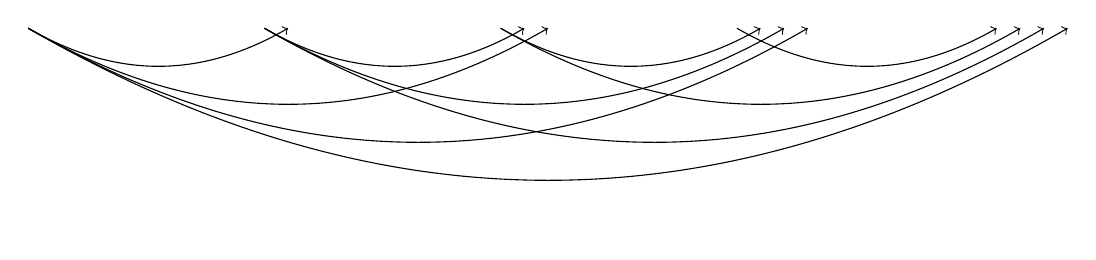
\begin{tikzpicture}
  \usetikzlibrary{3d}

  \def\scale{3}
  \def\netx{0}
  \def\nety{0}
  \def\netz{0}

  \def\coblue{blue!50!gray}
  \def\copurple{purple!50!gray}
  \def\coorange{orange!70!gray}
  \def\cogreen{green!50!gray}
  \def\copink{pink!50!gray}
  \def\comagenta{magenta!50!gray}
  \def\coyellow{yellow!50!white}
  \def\cored{red!50!white}

  \def\zoff{\netz+0.5*\scale}
  \def\yoff{\nety-0.5*\scale}
  \newcommand\denselink[2]{%
      \draw[->] (#1, \yoff, \zoff) to[bend right=30] (#2, \yoff, \zoff);
  }

  \convlayer{1*\scale}{1*\scale}{0.1*\scale}{Carte d'activation}{\copurple}{0.*\scale+\netx}{\nety}{\netz}{{}{}{}}
  \denselink{\netx+0*\scale}{\netx+1.1*\scale}
  \denselink{\netx+0*\scale}{\netx+2.2*\scale}
  \denselink{\netx+0*\scale}{\netx+3.3*\scale}
  \denselink{\netx+0*\scale}{\netx+4.4*\scale}

  \convlayer{1*\scale}{1*\scale}{0.1*\scale}{BN-ReLU-Conv}{\coblue}{\netx+1*\scale}{\nety}{\netz}{{}{}{}}
  \denselink{\netx+1*\scale}{\netx+2.1*\scale}
  \denselink{\netx+1*\scale}{\netx+3.2*\scale}
  \denselink{\netx+1*\scale}{\netx+4.3*\scale}

  \denselink{\netx+2*\scale}{\netx+3.1*\scale}
  \denselink{\netx+2*\scale}{\netx+4.2*\scale}

  \denselink{\netx+3*\scale}{\netx+4.1*\scale}

  \convlayer{1*\scale}{1*\scale}{0.1*\scale}{}{\copurple}{1.1*\scale+\netx}{\nety}{\netz}{{}{}{}}

  \convlayer{1*\scale}{1*\scale}{0.1*\scale}{BN-ReLU-Conv}{\copink}{\netx+2*\scale}{\nety}{\netz}{{}{}{}}
  \convlayer{1*\scale}{1*\scale}{0.1*\scale}{}{\coblue}{2.1*\scale+\netx}{\nety}{\netz}{{}{}{}}
  \convlayer{1*\scale}{1*\scale}{0.1*\scale}{}{\copurple}{2.2*\scale+\netx}{\nety}{\netz}{{}{}{}}

  \convlayer{1*\scale}{1*\scale}{0.1*\scale}{BN-ReLU-Conv}{\cored}{\netx+3*\scale}{\nety}{\netz}{{}{}{}}
  \convlayer{1*\scale}{1*\scale}{0.1*\scale}{}{\copink}{3.1*\scale+\netx}{\nety}{\netz}{{}{}{}}
  \convlayer{1*\scale}{1*\scale}{0.1*\scale}{}{\coblue}{3.2*\scale+\netx}{\nety}{\netz}{{}{}{}}
  \convlayer{1*\scale}{1*\scale}{0.1*\scale}{}{\copurple}{3.3*\scale+\netx}{\nety}{\netz}{{}{}{}}

  \convlayer{1*\scale}{1*\scale}{0.1*\scale}{BN-ReLU-Conv}{\comagenta}{\netx+4*\scale}{\nety}{\netz}{{}{}{}}
  \convlayer{1*\scale}{1*\scale}{0.1*\scale}{}{\cored}{4.1*\scale+\netx}{\nety}{\netz}{{}{}{}}
  \convlayer{1*\scale}{1*\scale}{0.1*\scale}{}{\copink}{4.2*\scale+\netx}{\nety}{\netz}{{}{}{}}
  \convlayer{1*\scale}{1*\scale}{0.1*\scale}{}{\coblue}{4.3*\scale+\netx}{\nety}{\netz}{{}{}{}}
  \convlayer{1*\scale}{1*\scale}{0.1*\scale}{}{\copurple}{4.4*\scale+\netx}{\nety}{\netz}{{}{}{}}

  \convlayer{1*\scale}{1*\scale}{0.2*\scale}{Transition}{\coyellow}{\netx+5.1*\scale}{\nety}{\netz}{{}{}{}}
  \convlayer{0.6*\scale}{0.6*\scale}{0.2*\scale}{Pooling}{\coorange}{\netx+5.7*\scale}{\nety}{\netz}{{}{}{}}
  \end{tikzpicture}
\end{document}

  }
  \caption{Bloc convolutif dense~\cite{huang_densely_2017}}
  \label{fig:denseblock}
  \end{minipage}
\end{figure}

En parallèle, \citet{szegedy_going_2015} proposent le modèle GoogLeNet avec 22 couches. Cette architecture introduit notamment le module \emph{Inception} empilant plusieurs couches en parallèle, et plus seulement en profondeur. L'idée est de réaliser, pour une carte d'activation, l'extraction de caractéristiques à plusieurs niveaux de contextes en utilisant soit une convolution $1\times1$, c'est-à-dire une combinaison linéaire suivie d'une non-linéarité, soit un \emph{pooling}, soit des convolutions $3\times3$ ou $5\times5$. Cela permet de coupler des caractéristiques dotées de l'invariance aux translations locales (issues du sous-échantillonnage) et des caractéristiques qui ne le sont pas, permettant donc de traiter une plus grande variété de cas. Le module \emph{Inception} est illustré dans la~\cref{fig:inception}. L'architecture complète du modèle GoogLeNet est détaillée dans la~\cref{fig:googlenet}. Compte-tenu de la profondeur du réseau (22 couches), ses auteurs proposent de faciliter l'optimisation des couches les plus basses en ajoutant un classifieur au niveau des représentations intermédiaires, après les modules \emph{Inception} (4a) et (4d), cette approche ayant déjà montré son efficacité pour lutter contre les problèmes de gradients évanescents par le passé~\cite{lee_deeply-supervised_2015}. Ce modèle obtient un taux d'ereur de seulement 6,4\% en reconnaissance d'objets à l'\gls{ILSVRC}. Ce modèle sera amélioré~\cite{szegedy_rethinking_2015} par la suite en remplaçant les convolutions $5\times5$ du module \emph{Inception} par deux convolutions $3\times3$, comme proposé dans le modèle VGG~\cite{simonyan_very_2014} et en intégrant la \emph{Batch Normalization}~\cite{ioffe_batch_2015}.
\todo[inline]{ajouter la supervision profonde au graphique Inception + LRN après Pool1 et Pool2}

\begin{figure}[t]
  \resizebox{\textwidth}{!}{
    \documentclass{standalone}
\usepackage[utf8]{inputenc}
\usepackage[T1]{fontenc}
\usepackage{tikz}
\usepackage{ifthen}
\usepackage{graphicx}
%%%%%%%%%%%%%%%%%%%%%%%%%%%%%%%%%%%%%%%%
%           Commandes perso            %
%%%%%%%%%%%%%%%%%%%%%%%%%%%%%%%%%%%%%%%%

%% Figures centrées, et en position 'here, top, bottom or page'
\newenvironment{figureth}{%
		\begin{figure}[htbp]
			\centering
	}{
		\end{figure}
		}


%% Tableaux centrés, et en position 'here, top, bottom or page'
\newenvironment{tableth}{%
		\begin{table}[htbp]
			\centering
			%\rowcolors{1}{coleurtableau}{coleurtableau}
	}{
		\end{table}
		}

%% Sous-figures centrées, en position 'top'
\newenvironment{subfigureth}[1]{%
	\begin{subfigure}[t]{#1}
	\centering
}{
	\end{subfigure}
}

\newcommand{\citationChap}[2]{%
	\epigraph{\og \textit{#1} \fg{}}{#2}
}

%% On commence par une page impaire quand on change le style de numérotation de pages
\let\oldpagenumbering\pagenumbering
\renewcommand{\pagenumbering}[1]{%
	\cleardoublepage
	\oldpagenumbering{#1}
}

%% Légende du dataset ISPRS
\newcommand\isprslegende{
Légende\,: \textcolor{Black}{blanc}\,: routes, \textcolor{Blue}{bleu}\,: bâtiments, \textcolor{Cerulean}{cyan}\,: végétation basse, \textcolor{OliveGreen}{vert}\,: arbres, \textcolor{Dandelion}{jaune}\,: véhicules, \textcolor{BrickRed}{rouge}\,: autre.
}

%% Dessiner des réseaux de neurones avec Tikz
\newcommand{\convlayer}[9]{%{h}{w}{d}{name}{color}{x}{y}{z}%{note w}{note h}{note d}
   \def\h{#1}
   \def\w{#2}
   \def\d{#3}
   \def\name{#4}
   \ifthenelse {\equal{#5} {}} {\def\col{white}} {\def\col{#5}}
   \def\x{#6}
   \ifthenelse {\equal{#7} {}} {\def\y{0}} {\def\y{#7}}
   \ifthenelse {\equal{#8} {}} {\def\z{0}} {\def\z{#8}}
   % ne faites pas ça chez vous !
   \ifthenelse {\equal{#9} {}} {\convlayercontinued{}{}{}} {\convlayercontinued#9}
}

\newcommand\convlayercontinued[3]{
   \def\notew{#1}
   \def\noteh{#2}
   \def\noted{#3}
   \coordinate (A) at (\x-\d/2,  \y-\h/2, \z-\w/2);
   \coordinate (B) at (\x-\d/2,  \y-\h/2, \z+\w/2);
   \coordinate (C) at (\x-\d/2,  \y+\h/2, \z+\w/2);
   \coordinate (D) at (\x-\d/2,  \y+\h/2, \z-\w/2);
   \coordinate (E) at (\x+\d/2,  \y-\h/2, \z-\w/2);
   \coordinate (F) at (\x+\d/2,  \y-\h/2, \z+\w/2);
   \coordinate (G) at (\x+\d/2,  \y+\h/2, \z+\w/2);
   \coordinate (H) at (\x+\d/2,  \y+\h/2, \z-\w/2);

    \draw [draw opacity=0.3, fill opacity=0.8, fill=\col!60!white] (A) -- (B) -- (C) -- (D) -- cycle;
    \draw [draw opacity=0.3, fill opacity=0.8, fill=\col!60!white] (A) -- (B) -- (F) -- (E) -- cycle;
    % Face haut
    %\draw [left color=\col!60!white, right color=\col!80!white, shading=axis, shading angle=180] (C) -- (D)  -- (H) -- (G) -- cycle;
    \draw [fill opacity=0.9, fill=\col!70!white] (C) -- node[rotate=45,above] {\small \name} (D) -- (H) -- (G) -- cycle;
    %\draw [fill opacity=0.9, fill=\col!70!white] (C) -- (D) -- node[above] {\small \name} (H) -- (G) -- cycle;
    % Face droite
    \draw [fill opacity=0.9, fill=\col!60!white] (E) -- node[pos=0.75,rotate=45,below] {\scriptsize \notew} (F) -- (G) --  (H) -- cycle;
    % Face avant
    %\draw [shading=axis, left color=\col!60!white, right color=\col!40!white, shading angle=-45] (B) -- node[above,rotate=90] {\scriptsize \noteh} (C) -- (G) -- (F) -- node[below] {\scriptsize \noted}  cycle;
    \draw [fill opacity=0.9, fill=\col!50!white] (B) -- node[above,rotate=90] {\scriptsize \noteh} (C) -- (G) -- (F) -- node[below] {\scriptsize \noted}  cycle;
}

\newcommand{\fclayer}[8]{%{h}{w}{name}{color}{x}{y}{z}
   \def\h{#1}
   \def\w{#2}
   \def\name{#3}
   \ifthenelse {\equal{#4} {}} {\def\col{white}} {\def\col{#4}}
   \def\x{#5}
   \def\y{#6}
   \def\z{#7}
   \def\note{#8}
   \coordinate (A) at (\x-\w/2,  \y-\h/2, \z);
   \coordinate (B) at (\x+\w/2,  \y-\h/2, \z);
   \coordinate (C) at (\x+\w/2,  \y+\h/2, \z);
   \coordinate (D) at (\x-\w/2,  \y+\h/2, \z);

   \pgfmathparse{4*\w}\let\boxwidth\pgfmathresult
    \draw [fill=\col] (A) -- node[below,text width=\boxwidth cm,align=center] {\scriptsize \note} (B) -- (C) -- (D) -- cycle;

    \node (N) at ($(A)!0.5!(B)+(0,-1,0)$) {\name};
}

\newcommand{\alexnet}[4]{%{scale}{x}{y}{z}
  \def\scale{#1}
  \def\alexx{#2}
  \def\alexy{#3}
  \def\alexz{#4}


  \def\coblue{blue!50!white}
  \def\fcgrey{gray!50!white}

  \convlayer{1.3*\scale}{1.3*\scale}{0.02*\scale}{Image}{\coblue}{\alexx}{\alexy}{\alexz}{{227}{227}{3}}
  \convlayer{1.1*\scale}{1.1*\scale}{0.08*\scale}{Conv1}{\coblue}{\alexx+0.7*\scale}{\alexy}{\alexz}{{55}{55}{96}}
  \convlayer{0.7*\scale}{0.7*\scale}{0.5*\scale}{Conv2}{\coblue}{\alexx+1.5*\scale}{\alexy}{\alexz}{{27}{27}{256}}
  \convlayer{0.5*\scale}{0.5*\scale}{0.8*\scale}{Conv3}{\coblue}{\alexx+2.6*\scale}{\alexy}{\alexz}{{13}{13}{384}}
  \convlayer{0.5*\scale}{0.5*\scale}{0.8*\scale}{Conv4}{\coblue}{\alexx+3.8*\scale}{\alexy}{\alexz}{{13}{13}{384}}
  \convlayer{0.5*\scale}{0.5*\scale}{0.5*\scale}{Conv5}{\coblue}{\alexx+4.8*\scale}{\alexy}{\alexz}{{13}{13}{256}}
  \fclayer{\scale}{0.1*\scale}{FC1}{\fcgrey}{\alexx+5.4*\scale}{\alexy}{\alexz}{4096}
  \fclayer{\scale}{0.1*\scale}{FC2}{\fcgrey}{\alexx+5.7*\scale}{\alexy}{\alexz}{4096}
  \fclayer{\scale}{0.1*\scale}{FC3}{\fcgrey}{\alexx+6.0*\scale}{\alexy}{\alexz}{1000}
}

\newcommand{\imagelayer}[7]{%{width}{x}{y}{z}{path}{text_up}{text_down}
    \pgfmathparse{#1}\let\w\pgfmathresult
    \begin{scope}[canvas is yz plane at x=#2]
     \node[transform shape] (source) at (#3, #4) {\includegraphics[angle=-90,width=\w cm]{#5}};
    \end{scope}
     \node [transform shape, rotate=45, above] at (source.east) {#6};
     \node [transform shape, rotate=45, below] at (source.west) {\scriptsize{#7}};
}

\def\fourier{\mathcal{F}}

\newcommand{\lightspectrum}{%
\pgfplotsset{
    % this *defines* a custom colormap ...
    colormap={slategraywhite}{color(0cm)=(red); color(1cm)=(red); color(2cm)=(red); color(3cm)=(red); color(4cm)=(orange); color(5cm)=(yellow); color(6cm)=(green); color(7cm)=(blue); color(8cm)=(blue); color(9cm)=(purple); color(10cm)=(purple); color(12cm)=(black)}
}
\node at (1.5, 2.7) {\small 1mm};
\node at (4, 3) {Infrarouge};
\node at (7.75, 2.7) {\small 800nm};
\node at (9, 3) {Visible};
\node at (10.5, 2.7) {\small 400nm};
\node at (12, 3) {Ultraviolet};
\node at (13.5, 2.7) {\small 10nm};
\draw[->] (1, 2.5) -- (14, 2.5);
\begin{axis}[hide axis,width=16cm,height=4cm,colormap name=slategraywhite]
\addplot[domain=20:1000,samples=1500,ultra thick, point meta=x*x,mesh]{sin(x*x/80)};
\end{axis}
}

% Union généralisée
\newcommand{\wbigcup}{\mathop{\bigcup}\displaylimits}

\newcommand{\res}[2]{#1 {\footnotesize $\pm$ #2}}
\newcommand{\bres}[2]{\textbf{#1} {\footnotesize $\pm$ #2}}
\newcommand{\bbres}[2]{\res{\textit{#1}}{#2}}

\newcommand{\drawkernel}[9]{
\begin{tikzpicture}
	\draw[step=1cm,gray!50!white,very thin] (0,0) grid (3,3);
	\kernelnode{0.5}{0.5}{#1};
	\kernelnode{0.5}{1.5}{#2};
	\kernelnode{0.5}{2.5}{#3};
	\kernelnode{1.5}{0.5}{#4};
	\kernelnode{1.5}{1.5}{#5};
	\kernelnode{1.5}{2.5}{#6};
	\kernelnode{2.5}{0.5}{#7};
	\kernelnode{2.5}{1.5}{#8};
	\kernelnode{2.5}{2.5}{#9};
\end{tikzpicture}
}

\newcommand{\kernelnode}[3]{%{x}{y}{value}
	\ifthenelse{\equal{#3}{0}}{
		\def\kcolor{gray}
	}{
		\def\kcolor{black}
	}
	\node[\kcolor] at (#1, #2) {#3};
}

\newcommand{\chapsummary}[1]{
\section*{Résumé du chapitre :}
\parbox{0.9\linewidth}{
\setlength{\parindent}{4ex}
#1}
}

\newcommand{\eqname}[1]{\tag*{\small (#1)}}


\begin{document}
  \begin{tikzpicture}
  \usetikzlibrary{calc}
  \usetikzlibrary{3d}

  \def\scale{4}
  \def\vggx{0}
  \def\vggy{0}
  \def\vggz{0}

  \def\coblue{blue!50!gray}
  \def\cored{red!50!gray}
  \def\coorange{orange!70!gray}
  \def\cogreen{green!50!gray}
  \def\copurple{purple!50!white}

  \imagelayer{1.3*\scale}{-0.3*\scale+\vggx}{\vggy}{\vggz}{nobu}{Image}{$224\times224\times3$}
  \convlayer{1.3*\scale}{1.3*\scale}{0.02*\scale}{Image}{\coblue}{0.2*\scale+\vggx}{\vggy}{\vggz}{{224}{}{3}}
  \convlayer{1*\scale}{1*\scale}{0.04*\scale}{Conv1}{\coblue}{\vggx+0.6*\scale}{\vggy}{\vggz}{{112}{112}{64}}
  \convlayer{0.8*\scale}{0.8*\scale}{0.04*\scale}{Pool1}{\coorange}{\vggx+1*\scale}{\vggy}{\vggz}{{56}{56}{}}

  \foreach \ratio [count=\ni] in {1.4,1.5,1.6,1.7,1.8,1.9}{
  \convlayer{0.8*\scale}{0.8*\scale}{0.04*\scale}{}{\coblue}{\vggx+\ratio*\scale}{\vggy}{\vggz}{{}{}{64}}
  \ifnum\ni=1%
      \draw (\vggx+\ratio*\scale-0.3*\scale, \vggy+0.5*\scale) edge[dashed,thick,->,in=90,out=90,looseness=2] (\vggx+\ratio*\scale, \vggy+0.4*\scale);
  \else%
      \draw (\vggx+\ratio*\scale-0.1*\scale+0.035*\scale, \vggy+0.4*\scale) edge[thick,->,in=90,out=90,looseness=10] (\vggx+\ratio*\scale, \vggy+0.4*\scale);
  \fi%
  }


  \foreach \ratio [count=\ni] in {2.2,2.35,2.5,2.65,2.8,2.95,3.10,3.25}{
  \convlayer{0.6*\scale}{0.6*\scale}{0.08*\scale}{}{\coblue}{\vggx+\ratio*\scale}{\vggy}{\vggz}{{}{}{128}}
  \ifnum\ni=1%
      \draw (\vggx+\ratio*\scale-0.2*\scale, \vggy+0.5*\scale) edge[dashed,looseness=2,thick,->,in=90,out=90] (\vggx+\ratio*\scale, \vggy+0.3*\scale);%
  \else%
      \draw (\vggx+\ratio*\scale-0.15*\scale+0.035*\scale, \vggy+0.3*\scale) edge[looseness=5,thick,->,in=90,out=90] (\vggx+\ratio*\scale, \vggy+0.3*\scale);%
  \fi%
  }

  \foreach \ratio [count=\ni] in {3.5,3.7,3.9,4.1,4.3,4.5,4.7,4.9,5.1,5.3,5.5,5.7}{
  \convlayer{0.4*\scale}{0.4*\scale}{0.12*\scale}{}{\coblue}{\vggx+\ratio*\scale}{\vggy}{\vggz}{{}{}{256}}
  \ifnum\ni=1%
      \draw (\vggx+\ratio*\scale-0.2*\scale, \vggy+0.3*\scale) edge[dashed,thick,looseness=1.5,->,in=90,out=90] (\vggx+\ratio*\scale, \vggy+0.2*\scale);
  \else%
      \draw (\vggx+\ratio*\scale-0.2*\scale+0.035*\scale, \vggy+0.2*\scale) edge[thick,looseness=2,->,in=90,out=90] (\vggx+\ratio*\scale, \vggy+0.2*\scale);
  \fi%
  }

  \foreach \ratio [count=\ni] in {6,6.3,6.6,6.9,7.2,7.5,7.8}{
  \convlayer{0.3*\scale}{0.3*\scale}{0.2*\scale}{}{\coblue}{\vggx+\ratio*\scale}{\vggy}{\vggz}{{}{}{512}}
  \ifnum\ni=1%
      \draw (\vggx+\ratio*\scale-0.3*\scale+0.05*\scale, \vggy+0.225*\scale) edge[dashed,thick,->,in=90,out=90,looseness=1.25] (\vggx+\ratio*\scale, \vggy+0.15*\scale);
  \else%
      \draw (\vggx+\ratio*\scale-0.3*\scale+0.05*\scale, \vggy+0.15*\scale) edge[thick,->,in=90,out=90,looseness=1.5] (\vggx+\ratio*\scale, \vggy+0.15*\scale);
  \fi%
  }

  \node at (\vggx+8.3*\scale, \vggy+0.2*\scale) {Avg. pool};
  \convlayer{0.1*\scale}{0.1*\scale}{0.6*\scale}{}{\coorange}{\vggx+8.3*\scale}{\vggy}{\vggz}{{}{}{$1\times1\times1024$}}
  \fclayer{\scale}{0.1*\scale}{FC}{\copurple}{\vggx+8.7*\scale}{\vggy}{\vggz}{1000}
  \node (out) at (\vggx+9.1*\scale,\vggy) {\Large ``Chat''};
  \draw[->] (\vggx+8.75*\scale,\vggy) -- (out.west);

  \end{tikzpicture}
\end{document}

  }
  \caption{Architecture ResNet-34~\cite{he_deep_2016}}
  \label{fig:resnet}
\end{figure}

En 2015, \citet{he_deep_2016} parviennent à obtenir un taux d'erreur de seulement 3,5\% en reconnaissance d'objet durant le \gls{ILSVRC}. Leur approche consiste en un réseau très profond comprenant plus de 100 couches convolutives. L'optimisation est rendue possible d'une part grâce à la \emph{Batch Normalization}, mais surtout grâce à l'apprentissage par résidu. L'idée est de briser la structure purement séquentielle des réseaux à propagation avant en ajoutant des connexions permettant de shunter la couche suivante. Ces connexions, dites résiduelles, correspondent à une simple opération identité et permettent alors aux activations et au gradient de parcourir l'ensemble du réseau sans subir d'évanescene ou d'explosion dues à la règle de la dérivation en chaîne. Plutôt de cherche à approximer $f\,: x \rightarrow f(x)$, le bloc résiduel va approximer $\hat{f}\,: x \rightarrow f(x) - x$, plus simple car d'amplitude a priori plus faible. Le bloc de convolution résiduel est illustré dans la~\cref{fig:residual} et un exemple de modèle dit \emph{ResNet} à 34 couches est détaillé dans la~\cref{fig:resnet}. L'introduction de l'apprentissage par résidu change en partie le paradigme utilisée jusqu'alors pour la conception des \gls{CNN}. Le bloc de base constitutif du réseau passe ainsi au bloc résiduel.
Les ResNet possèdent beaucoup de couches mais comparativement peu de paramètres, car seule la dernière couche est entièrement connectée. Comme nous l'avons vu, les couches entièrement connectées concentrent en général la majorité des poids des \gls{CNN} et sont également les plus sensibles au surapprentissage, nécessitant l'intégration de régularisations comme le \emph{Dropout}~\cite{srivastava_dropout_2014}. ResNet ne contient quasiment que des convolutions $3\times3$, à l'exception de la première $7\times7$ qui permet de réduire brutalement les dimensions spatiales de l'image. Il est intéressant de constater que la réduction de dimension finale avant la couche entièrement connectée se fait à l'aide d'un sous-échantillonnage adaptatif. Ainsi, peu importe la taille de l'image de l'entrée\,: le sous-échantillonnage moyennera les activations pour produire le vecteur de caractéristiques de taille attendue par la couche entièrement connectée. Cependant, il faut noter que le nombre élevé d'activations et de gradients intermédiaires à calculer rend les ResNet coûteux en mémoire et peu pratiques sur de grandes images. L'architecture \emph{Inception} sera également augmentée par des connexions résiduelles~\cite{szegedy_inception-v4_2016}.


\begin{figure}[t]
  \resizebox{\textwidth}{!}{
    \documentclass{standalone}
\usepackage[utf8]{inputenc}
\usepackage[T1]{fontenc}
\usepackage{tikz}
\usepackage{ifthen}
\usepackage{graphicx}
%%%%%%%%%%%%%%%%%%%%%%%%%%%%%%%%%%%%%%%%
%           Commandes perso            %
%%%%%%%%%%%%%%%%%%%%%%%%%%%%%%%%%%%%%%%%

%% Figures centrées, et en position 'here, top, bottom or page'
\newenvironment{figureth}{%
		\begin{figure}[htbp]
			\centering
	}{
		\end{figure}
		}


%% Tableaux centrés, et en position 'here, top, bottom or page'
\newenvironment{tableth}{%
		\begin{table}[htbp]
			\centering
			%\rowcolors{1}{coleurtableau}{coleurtableau}
	}{
		\end{table}
		}

%% Sous-figures centrées, en position 'top'
\newenvironment{subfigureth}[1]{%
	\begin{subfigure}[t]{#1}
	\centering
}{
	\end{subfigure}
}

\newcommand{\citationChap}[2]{%
	\epigraph{\og \textit{#1} \fg{}}{#2}
}

%% On commence par une page impaire quand on change le style de numérotation de pages
\let\oldpagenumbering\pagenumbering
\renewcommand{\pagenumbering}[1]{%
	\cleardoublepage
	\oldpagenumbering{#1}
}

%% Légende du dataset ISPRS
\newcommand\isprslegende{
Légende\,: \textcolor{Black}{blanc}\,: routes, \textcolor{Blue}{bleu}\,: bâtiments, \textcolor{Cerulean}{cyan}\,: végétation basse, \textcolor{OliveGreen}{vert}\,: arbres, \textcolor{Dandelion}{jaune}\,: véhicules, \textcolor{BrickRed}{rouge}\,: autre.
}

%% Dessiner des réseaux de neurones avec Tikz
\newcommand{\convlayer}[9]{%{h}{w}{d}{name}{color}{x}{y}{z}%{note w}{note h}{note d}
   \def\h{#1}
   \def\w{#2}
   \def\d{#3}
   \def\name{#4}
   \ifthenelse {\equal{#5} {}} {\def\col{white}} {\def\col{#5}}
   \def\x{#6}
   \ifthenelse {\equal{#7} {}} {\def\y{0}} {\def\y{#7}}
   \ifthenelse {\equal{#8} {}} {\def\z{0}} {\def\z{#8}}
   % ne faites pas ça chez vous !
   \ifthenelse {\equal{#9} {}} {\convlayercontinued{}{}{}} {\convlayercontinued#9}
}

\newcommand\convlayercontinued[3]{
   \def\notew{#1}
   \def\noteh{#2}
   \def\noted{#3}
   \coordinate (A) at (\x-\d/2,  \y-\h/2, \z-\w/2);
   \coordinate (B) at (\x-\d/2,  \y-\h/2, \z+\w/2);
   \coordinate (C) at (\x-\d/2,  \y+\h/2, \z+\w/2);
   \coordinate (D) at (\x-\d/2,  \y+\h/2, \z-\w/2);
   \coordinate (E) at (\x+\d/2,  \y-\h/2, \z-\w/2);
   \coordinate (F) at (\x+\d/2,  \y-\h/2, \z+\w/2);
   \coordinate (G) at (\x+\d/2,  \y+\h/2, \z+\w/2);
   \coordinate (H) at (\x+\d/2,  \y+\h/2, \z-\w/2);

    \draw [draw opacity=0.3, fill opacity=0.8, fill=\col!60!white] (A) -- (B) -- (C) -- (D) -- cycle;
    \draw [draw opacity=0.3, fill opacity=0.8, fill=\col!60!white] (A) -- (B) -- (F) -- (E) -- cycle;
    % Face haut
    %\draw [left color=\col!60!white, right color=\col!80!white, shading=axis, shading angle=180] (C) -- (D)  -- (H) -- (G) -- cycle;
    \draw [fill opacity=0.9, fill=\col!70!white] (C) -- node[rotate=45,above] {\small \name} (D) -- (H) -- (G) -- cycle;
    %\draw [fill opacity=0.9, fill=\col!70!white] (C) -- (D) -- node[above] {\small \name} (H) -- (G) -- cycle;
    % Face droite
    \draw [fill opacity=0.9, fill=\col!60!white] (E) -- node[pos=0.75,rotate=45,below] {\scriptsize \notew} (F) -- (G) --  (H) -- cycle;
    % Face avant
    %\draw [shading=axis, left color=\col!60!white, right color=\col!40!white, shading angle=-45] (B) -- node[above,rotate=90] {\scriptsize \noteh} (C) -- (G) -- (F) -- node[below] {\scriptsize \noted}  cycle;
    \draw [fill opacity=0.9, fill=\col!50!white] (B) -- node[above,rotate=90] {\scriptsize \noteh} (C) -- (G) -- (F) -- node[below] {\scriptsize \noted}  cycle;
}

\newcommand{\fclayer}[8]{%{h}{w}{name}{color}{x}{y}{z}
   \def\h{#1}
   \def\w{#2}
   \def\name{#3}
   \ifthenelse {\equal{#4} {}} {\def\col{white}} {\def\col{#4}}
   \def\x{#5}
   \def\y{#6}
   \def\z{#7}
   \def\note{#8}
   \coordinate (A) at (\x-\w/2,  \y-\h/2, \z);
   \coordinate (B) at (\x+\w/2,  \y-\h/2, \z);
   \coordinate (C) at (\x+\w/2,  \y+\h/2, \z);
   \coordinate (D) at (\x-\w/2,  \y+\h/2, \z);

   \pgfmathparse{4*\w}\let\boxwidth\pgfmathresult
    \draw [fill=\col] (A) -- node[below,text width=\boxwidth cm,align=center] {\scriptsize \note} (B) -- (C) -- (D) -- cycle;

    \node (N) at ($(A)!0.5!(B)+(0,-1,0)$) {\name};
}

\newcommand{\alexnet}[4]{%{scale}{x}{y}{z}
  \def\scale{#1}
  \def\alexx{#2}
  \def\alexy{#3}
  \def\alexz{#4}


  \def\coblue{blue!50!white}
  \def\fcgrey{gray!50!white}

  \convlayer{1.3*\scale}{1.3*\scale}{0.02*\scale}{Image}{\coblue}{\alexx}{\alexy}{\alexz}{{227}{227}{3}}
  \convlayer{1.1*\scale}{1.1*\scale}{0.08*\scale}{Conv1}{\coblue}{\alexx+0.7*\scale}{\alexy}{\alexz}{{55}{55}{96}}
  \convlayer{0.7*\scale}{0.7*\scale}{0.5*\scale}{Conv2}{\coblue}{\alexx+1.5*\scale}{\alexy}{\alexz}{{27}{27}{256}}
  \convlayer{0.5*\scale}{0.5*\scale}{0.8*\scale}{Conv3}{\coblue}{\alexx+2.6*\scale}{\alexy}{\alexz}{{13}{13}{384}}
  \convlayer{0.5*\scale}{0.5*\scale}{0.8*\scale}{Conv4}{\coblue}{\alexx+3.8*\scale}{\alexy}{\alexz}{{13}{13}{384}}
  \convlayer{0.5*\scale}{0.5*\scale}{0.5*\scale}{Conv5}{\coblue}{\alexx+4.8*\scale}{\alexy}{\alexz}{{13}{13}{256}}
  \fclayer{\scale}{0.1*\scale}{FC1}{\fcgrey}{\alexx+5.4*\scale}{\alexy}{\alexz}{4096}
  \fclayer{\scale}{0.1*\scale}{FC2}{\fcgrey}{\alexx+5.7*\scale}{\alexy}{\alexz}{4096}
  \fclayer{\scale}{0.1*\scale}{FC3}{\fcgrey}{\alexx+6.0*\scale}{\alexy}{\alexz}{1000}
}

\newcommand{\imagelayer}[7]{%{width}{x}{y}{z}{path}{text_up}{text_down}
    \pgfmathparse{#1}\let\w\pgfmathresult
    \begin{scope}[canvas is yz plane at x=#2]
     \node[transform shape] (source) at (#3, #4) {\includegraphics[angle=-90,width=\w cm]{#5}};
    \end{scope}
     \node [transform shape, rotate=45, above] at (source.east) {#6};
     \node [transform shape, rotate=45, below] at (source.west) {\scriptsize{#7}};
}

\def\fourier{\mathcal{F}}

\newcommand{\lightspectrum}{%
\pgfplotsset{
    % this *defines* a custom colormap ...
    colormap={slategraywhite}{color(0cm)=(red); color(1cm)=(red); color(2cm)=(red); color(3cm)=(red); color(4cm)=(orange); color(5cm)=(yellow); color(6cm)=(green); color(7cm)=(blue); color(8cm)=(blue); color(9cm)=(purple); color(10cm)=(purple); color(12cm)=(black)}
}
\node at (1.5, 2.7) {\small 1mm};
\node at (4, 3) {Infrarouge};
\node at (7.75, 2.7) {\small 800nm};
\node at (9, 3) {Visible};
\node at (10.5, 2.7) {\small 400nm};
\node at (12, 3) {Ultraviolet};
\node at (13.5, 2.7) {\small 10nm};
\draw[->] (1, 2.5) -- (14, 2.5);
\begin{axis}[hide axis,width=16cm,height=4cm,colormap name=slategraywhite]
\addplot[domain=20:1000,samples=1500,ultra thick, point meta=x*x,mesh]{sin(x*x/80)};
\end{axis}
}

% Union généralisée
\newcommand{\wbigcup}{\mathop{\bigcup}\displaylimits}

\newcommand{\res}[2]{#1 {\footnotesize $\pm$ #2}}
\newcommand{\bres}[2]{\textbf{#1} {\footnotesize $\pm$ #2}}
\newcommand{\bbres}[2]{\res{\textit{#1}}{#2}}

\newcommand{\drawkernel}[9]{
\begin{tikzpicture}
	\draw[step=1cm,gray!50!white,very thin] (0,0) grid (3,3);
	\kernelnode{0.5}{0.5}{#1};
	\kernelnode{0.5}{1.5}{#2};
	\kernelnode{0.5}{2.5}{#3};
	\kernelnode{1.5}{0.5}{#4};
	\kernelnode{1.5}{1.5}{#5};
	\kernelnode{1.5}{2.5}{#6};
	\kernelnode{2.5}{0.5}{#7};
	\kernelnode{2.5}{1.5}{#8};
	\kernelnode{2.5}{2.5}{#9};
\end{tikzpicture}
}

\newcommand{\kernelnode}[3]{%{x}{y}{value}
	\ifthenelse{\equal{#3}{0}}{
		\def\kcolor{gray}
	}{
		\def\kcolor{black}
	}
	\node[\kcolor] at (#1, #2) {#3};
}

\newcommand{\chapsummary}[1]{
\section*{Résumé du chapitre :}
\parbox{0.9\linewidth}{
\setlength{\parindent}{4ex}
#1}
}

\newcommand{\eqname}[1]{\tag*{\small (#1)}}


\begin{document}
  \begin{tikzpicture}
  \usetikzlibrary{calc}
  \usetikzlibrary{3d}

  \def\scale{4}
  \def\vggx{0}
  \def\vggy{0}
  \def\vggz{0}

  \def\coblue{blue!50!gray}
  \def\cored{red!50!gray}
  \def\coorange{orange!70!gray}
  \def\cogreen{green!50!gray}
  \def\copurple{purple!50!white}

  \imagelayer{1.3*\scale}{-0.3*\scale+\vggx}{\vggy}{\vggz}{nobu}{Image}{$224\times224\times3$}
  \convlayer{1.3*\scale}{1.3*\scale}{0.01*\scale}{Image}{\coblue}{0.2*\scale+\vggx}{\vggy}{\vggz}{{224}{}{3}}
  \convlayer{1*\scale}{1*\scale}{0.02*\scale}{Conv1}{\coblue}{\vggx+0.6*\scale}{\vggy}{\vggz}{{112}{112}{64}}
  \convlayer{0.8*\scale}{0.8*\scale}{0.02*\scale}{Pool1}{\coorange}{\vggx+1*\scale}{\vggy}{\vggz}{{56}{56}{}}

  \foreach \ratio [count=\ni] in {1.4,1.44,...,2.28}{
  \convlayer{0.8*\scale}{0.8*\scale}{0.04*\scale}{}{\cored}{\vggx+\ratio*\scale}{\vggy}{\vggz}{{}{}{}}
  }

  \convlayer{0.6*\scale}{0.6*\scale}{0.04*\scale}{Transition}{\coblue}{\vggx+2.5*\scale}{\vggy}{\vggz}{{}{}{}}

  \foreach \ratio [count=\ni] in {2.75,2.79,...,3.71}{
  \convlayer{0.6*\scale}{0.6*\scale}{0.04*\scale}{}{\cored}{\vggx+\ratio*\scale}{\vggy}{\vggz}{{}{}{}}
  }

  \convlayer{0.4*\scale}{0.4*\scale}{0.04*\scale}{Transition}{\coblue}{\vggx+4*\scale}{\vggy}{\vggz}{{}{}{}}

  \foreach \ratio [count=\ni] in {4.2,4.24,...,6.04}{
  \convlayer{0.4*\scale}{0.4*\scale}{0.04*\scale}{}{\cored}{\vggx+\ratio*\scale}{\vggy}{\vggz}{{}{}{}}
  }

  \convlayer{0.2*\scale}{0.2*\scale}{0.04*\scale}{Transition}{\coblue}{\vggx+6.25*\scale}{\vggy}{\vggz}{{}{}{}}

  \foreach \ratio [count=\ni] in {6.5,6.54,...,7.28}{
  \convlayer{0.2*\scale}{0.2*\scale}{0.04*\scale}{}{\cored}{\vggx+\ratio*\scale}{\vggy}{\vggz}{{}{}{}}
  }

  \node at (\vggx+8.3*\scale, \vggy+0.2*\scale) {Avg. pool};
  \convlayer{0.1*\scale}{0.1*\scale}{0.6*\scale}{}{\coorange}{\vggx+8.3*\scale}{\vggy}{\vggz}{{}{}{$1\times1\times1024$}}
  \fclayer{\scale}{0.1*\scale}{FC}{\copurple}{\vggx+8.7*\scale}{\vggy}{\vggz}{1000}
  \node (out) at (\vggx+9.1*\scale,\vggy) {\Large ``Chat''};
  \draw[->] (\vggx+8.75*\scale,\vggy) -- (out.west);

  \end{tikzpicture}
\end{document}

  }
  \caption{Architecture DenseNet-121~\cite{huang_densely_2017}}
  \label{fig:densenet}
\end{figure}


L'utilisation de cartes d'activation intermédiaires et leur propagation aux couches supérieures permet une meilleure classification en prenant en compte plusieurs niveaux d'abstraction. Toutefois, les connexions résiduelles ne permettent que d'accéder aux activations de la couche précédente. \citet{huang_densely_2017} ont donc proposé une architecture dite \emph{DenseNet} comportant des connexions denses, construisant un modèle au sein duquel toutes les cartes d'activation issues des couches inférieures sont transmises à toutes les couches supérieures. Pour éviter l'explosion du nombre de paramètres et d'activations, le modèle est divisé en plusieurs blocs denses, comme illustré dans la~\cref{fig:densenet}. Chaque bloc se détaille comme illustré dans la~\cref{fig:denseblock}. La présence des connexions denses permet au gradient de se propager immédiatement des couches supérieures aux couches inférieures, appliquant ainsi une forme implicite de supervision profonde~\cite{lee_deeply-supervised_2015}. Entre deux blocs, une couche convolutive de transition set appliquée pour réduire le nombre de plans et est suivie d'un \emph{max-pooling} pour réduire les dimensions spatiales. Cette architecture obtient comparativement de meilleurs résultats que les modèles ResNet sur la base de validation de l'\gls{ILSVRC}2012. Toutefois, comme pour les ResNet, si le nombre de paramètres des architectures DenseNet est faible, ils sont coûteux en espace mémoire nécessaire pour stocker les activations et gradients intermédiaires.

\todo[inline]{depthwise/separable convolutions}


Toutefois, la classification d'images ne donne aucune information particulière de localisation, seulement une information binaire de présence d'un objet dans une image. Les premières approches se sont intéressés au calcul de caractéristiques denses sur l'image associées à des cascades multi-échelles de classifieurs pour détecter des objets dans chaque sous-région de l'image. C'est l'approche utilisée par les descripteurs \gls{SIFT}~\cite{lowe_object_1999}, les pseudo-Haar de la méthode de Viola et Jones~\cite{viola_robust_2001} ou encore des \gls{HOG}~\cite{dalal_histograms_2005}. Des approches à base de réseaux profonds pour la détection d'objet à partir de classification de sous-régions de l'image ont rapidement vu le jour~\cite{girshick_rich_2014,liu_ssd_2016,girshick_region-based_2016} supplantant les approches traditionnelles de localisation à partir d'extraction de fenêtres candidates~\cite{gu_recognition_2009,uijlings_selective_2013}. L'idée principale tourne toujours autour d'une extraction dense de caractéristique et de l'identification de régions de l'image susceptibles de contenir un des objets d'intérêt. Cependant, ces approches ne répondent pas exactement au problème décrit par Papert en 1966. La question n'est pas uniquement de pouvoir identifier des objets, mais aussi d'en estimer la forme et de les séparer du fond, comme illustré dans la~\cref{fig:classif_vs_seg}. Cette tâche consiste donc à la segmentation sémantique, c'est-à-dire à l'association d'une classe d'intérêt non pas à chaque image, mais à chaque pixel.

Plusieurs jeux de données ont été introduits dans la communauté vision par ordinateur afin d'évaluer des méthodes sur cette tâche, notamment sur des scènes de la vie quotidienne, comme PASCAL VOC~\cite{everingham_pascal_2014}, Microsoft COCO~\cite{lin_microsoft_2014} et également sur des scènes de conduite autonome avec des jeux de données tels que CamVid~\cite{brostow_semantic_2009}, Cityscapes~\cite{cordts_cityscapes_2016} ou encore Mapillary Vistas~\cite{neuhold_mapillary_2017}. Les premières approches de segmentation sémantique ont réalisé des classification à partir de caractéristiques denses calculées sur l'ensemble de l'image, regroupées \emph{a posteriori} par régions homogènes~\cite{shotton_semantic_2008,shotton_real-time_2011}. Les réseaux convolutifs profonds également utilisés à cette fin en calculant une classification pour chaque pixel de l'image~\cite{grangier_deep_2009,ciresan_deep_2012} ou pour chaque région~\cite{farabet_towards_2013,sermanet_overfeat_2013}. Une observation importante est que les cartes de caractéristiques issues des couches convolutives conservent la structure spatiale de l'image, c'est-à-dire qu'il est possible de faire correspondre chaque caractéristique à un ou plusieurs pixels. Cette extraction de caractéristique dense se prête particulièrement aux problématiques de localisation d'objet et est rapidement adoptée par la communauté~\cite{zou_generic_2014}.

\subsection{Approches entièrement convolutives}

\missingfigure{Convolutionalisation}

La forme moderne des réseaux convolutifs profonds pour la segmentation sémantique est popularisée par~\citet{long_fully_2015}. L'idée fondamentale est de ne manipuler que des réseaux entièrement convolutifs, c'est-à-dire sans couche entièrement connectées. Dès lors, les cartes d'activation conservent leurs propriétés spatiales et peuvent être relocalisées sur l'image originale par un simple jeu de sur-échantillonnage, par exemple par interpolation bilinéaire. L'approche choisie par~\citet{long_fully_2015} leur permet de produire des prédictions denses à résolution 1:32, 1:16 et 1:8. Cette approche permettent immédiatement d'établir de nouveaux état de l'art sur les jeux de données de segmentation sémantique et dominent largement les compétitions depuis 2015.

Cette approche est reprise et améliorée selon plusieurs axes. Tout d'abord, en gardant la structure des couches convolutives de VGG-16~\cite{simonyan_very_2014},~\citet{l._c._chen_deeplab_2018} proposent d'une part d'utiliser les convolutions à trous pour agrandir le champ réceptif du réseau et retirer les couches de \emph{maxpooling} qui réduisent la résolution spatiale, et d'autre part d'utiliser un \gls{CRF} \emph{a posteriori} pour régulariser les cartes prédites. De façon similaire,~\citet{yu_multi-scale_2015} proposent l'utilisation de la convolution à trous (nommée convolution dilatée) pour agréger des cartes d'activation à plusieurs échelles. Les \gls{CRF} sont également manipulés de manière à s'exprimer sous forme d'un réseau récurrent optimisable conjointement avec le \gls{FCN}~\cite{zheng_conditional_2015} ou comme rafinement~\cite{arnab_higher_2015}.

Une approche dérivée des auto-encodeurs convolutifs~\cite{zhao_stacked_2015-1} est proposée, en utilisant soit la déconvolution pour recomposer la résolution spatiale~\cite{ronneberger_u-net_2015,nekrasov_global_2016,noh_learning_2015}, soit le sur-échantillonnage~\cite{badrinarayanan_segnet_2017}.

Le passage aux architectures ResNet~\cite{wu_high-performance_2016} puis DenseNet~\cite{jegou_one_2017} permettent d'améliorer encore les performances mais au prix d'un surcoût calculatoire conséquent.

\todo[inline]{large kernel matters (papier), gridnet (papier)}
Diverses approches multi-échelles sont proposées, aussi bien dans DeepLab~\cite{l._c._chen_deeplab_2018} en utilisant des prédictions à plusieurs résolutions que par des approches utilisant des noyaux de convolution à différentes tailles, soit via la dilation~\cite{yu_multi-scale_2015}, soit par des convolutions parallèle à la Inception~\cite{szegedy_going_2015,nekrasov_global_2016,zhao_pyramid_2017}.

\section{Apprentissage pour le traitement d'images de télédétection}

\subsection{Différents types d'imagerie}

La télédétection et en particulier l'observation de la Terre comprend une grande variété de capteurs d'imageries. Contrairement au multimédia, ces capteurs peuvent être de nature très variables. Si les acquisitions aéroportées se font généralement en couleurs \gls{RVB} à l'aide d'appareils photos clasiques, les acquisitions satellitaires utilisent bien souvent des capteurs dotés de capacités particulière, comme de remonter une information spectrale riche, percer la couverture nuageuse ou mesurer des propriétés physiques de la surface de la Terre.

Le cas plus simple à envisager est celui de l'infrarouge. Il est courant, y compris dans les acquisitions d'images aéroportées, d'imager aussi bien le domaine visible que le proche infrarouge, situé entre \SI{780}{\nano\meter} et \SI{2 500}{\nano\meter}, notamment car la végétation y a une réponse amplifiée par la présence de chlorophylle. Dans l'infrarouge moyen et lointain, il est également possible de mesurer indirectement la température grâce aux radiations lumineuses émises grâce à la loi de Wien. Ces caméras thermiques sont particulièrement utiles dans l'espace, car cela permet de s'affranchir du bruit ambiant causé par la chaleur naturelle terrestre.

\begin{figure}
  \resizebox{\textwidth}{!}{
  \documentclass{standalone}
\usepackage[utf8]{inputenc}
\usepackage[T1]{fontenc}
\usepackage{tikz}
\usepackage{pgfplots}
%%%%%%%%%%%%%%%%%%%%%%%%%%%%%%%%%%%%%%%%
%           Commandes perso            %
%%%%%%%%%%%%%%%%%%%%%%%%%%%%%%%%%%%%%%%%

%% Figures centrées, et en position 'here, top, bottom or page'
\newenvironment{figureth}{%
		\begin{figure}[htbp]
			\centering
	}{
		\end{figure}
		}


%% Tableaux centrés, et en position 'here, top, bottom or page'
\newenvironment{tableth}{%
		\begin{table}[htbp]
			\centering
			%\rowcolors{1}{coleurtableau}{coleurtableau}
	}{
		\end{table}
		}

%% Sous-figures centrées, en position 'top'
\newenvironment{subfigureth}[1]{%
	\begin{subfigure}[t]{#1}
	\centering
}{
	\end{subfigure}
}

\newcommand{\citationChap}[2]{%
	\epigraph{\og \textit{#1} \fg{}}{#2}
}

%% On commence par une page impaire quand on change le style de numérotation de pages
\let\oldpagenumbering\pagenumbering
\renewcommand{\pagenumbering}[1]{%
	\cleardoublepage
	\oldpagenumbering{#1}
}

%% Légende du dataset ISPRS
\newcommand\isprslegende{
Légende\,: \textcolor{Black}{blanc}\,: routes, \textcolor{Blue}{bleu}\,: bâtiments, \textcolor{Cerulean}{cyan}\,: végétation basse, \textcolor{OliveGreen}{vert}\,: arbres, \textcolor{Dandelion}{jaune}\,: véhicules, \textcolor{BrickRed}{rouge}\,: autre.
}

%% Dessiner des réseaux de neurones avec Tikz
\newcommand{\convlayer}[9]{%{h}{w}{d}{name}{color}{x}{y}{z}%{note w}{note h}{note d}
   \def\h{#1}
   \def\w{#2}
   \def\d{#3}
   \def\name{#4}
   \ifthenelse {\equal{#5} {}} {\def\col{white}} {\def\col{#5}}
   \def\x{#6}
   \ifthenelse {\equal{#7} {}} {\def\y{0}} {\def\y{#7}}
   \ifthenelse {\equal{#8} {}} {\def\z{0}} {\def\z{#8}}
   % ne faites pas ça chez vous !
   \ifthenelse {\equal{#9} {}} {\convlayercontinued{}{}{}} {\convlayercontinued#9}
}

\newcommand\convlayercontinued[3]{
   \def\notew{#1}
   \def\noteh{#2}
   \def\noted{#3}
   \coordinate (A) at (\x-\d/2,  \y-\h/2, \z-\w/2);
   \coordinate (B) at (\x-\d/2,  \y-\h/2, \z+\w/2);
   \coordinate (C) at (\x-\d/2,  \y+\h/2, \z+\w/2);
   \coordinate (D) at (\x-\d/2,  \y+\h/2, \z-\w/2);
   \coordinate (E) at (\x+\d/2,  \y-\h/2, \z-\w/2);
   \coordinate (F) at (\x+\d/2,  \y-\h/2, \z+\w/2);
   \coordinate (G) at (\x+\d/2,  \y+\h/2, \z+\w/2);
   \coordinate (H) at (\x+\d/2,  \y+\h/2, \z-\w/2);

    \draw [draw opacity=0.3, fill opacity=0.8, fill=\col!60!white] (A) -- (B) -- (C) -- (D) -- cycle;
    \draw [draw opacity=0.3, fill opacity=0.8, fill=\col!60!white] (A) -- (B) -- (F) -- (E) -- cycle;
    % Face haut
    %\draw [left color=\col!60!white, right color=\col!80!white, shading=axis, shading angle=180] (C) -- (D)  -- (H) -- (G) -- cycle;
    \draw [fill opacity=0.9, fill=\col!70!white] (C) -- node[rotate=45,above] {\small \name} (D) -- (H) -- (G) -- cycle;
    %\draw [fill opacity=0.9, fill=\col!70!white] (C) -- (D) -- node[above] {\small \name} (H) -- (G) -- cycle;
    % Face droite
    \draw [fill opacity=0.9, fill=\col!60!white] (E) -- node[pos=0.75,rotate=45,below] {\scriptsize \notew} (F) -- (G) --  (H) -- cycle;
    % Face avant
    %\draw [shading=axis, left color=\col!60!white, right color=\col!40!white, shading angle=-45] (B) -- node[above,rotate=90] {\scriptsize \noteh} (C) -- (G) -- (F) -- node[below] {\scriptsize \noted}  cycle;
    \draw [fill opacity=0.9, fill=\col!50!white] (B) -- node[above,rotate=90] {\scriptsize \noteh} (C) -- (G) -- (F) -- node[below] {\scriptsize \noted}  cycle;
}

\newcommand{\fclayer}[8]{%{h}{w}{name}{color}{x}{y}{z}
   \def\h{#1}
   \def\w{#2}
   \def\name{#3}
   \ifthenelse {\equal{#4} {}} {\def\col{white}} {\def\col{#4}}
   \def\x{#5}
   \def\y{#6}
   \def\z{#7}
   \def\note{#8}
   \coordinate (A) at (\x-\w/2,  \y-\h/2, \z);
   \coordinate (B) at (\x+\w/2,  \y-\h/2, \z);
   \coordinate (C) at (\x+\w/2,  \y+\h/2, \z);
   \coordinate (D) at (\x-\w/2,  \y+\h/2, \z);

   \pgfmathparse{4*\w}\let\boxwidth\pgfmathresult
    \draw [fill=\col] (A) -- node[below,text width=\boxwidth cm,align=center] {\scriptsize \note} (B) -- (C) -- (D) -- cycle;

    \node (N) at ($(A)!0.5!(B)+(0,-1,0)$) {\name};
}

\newcommand{\alexnet}[4]{%{scale}{x}{y}{z}
  \def\scale{#1}
  \def\alexx{#2}
  \def\alexy{#3}
  \def\alexz{#4}


  \def\coblue{blue!50!white}
  \def\fcgrey{gray!50!white}

  \convlayer{1.3*\scale}{1.3*\scale}{0.02*\scale}{Image}{\coblue}{\alexx}{\alexy}{\alexz}{{227}{227}{3}}
  \convlayer{1.1*\scale}{1.1*\scale}{0.08*\scale}{Conv1}{\coblue}{\alexx+0.7*\scale}{\alexy}{\alexz}{{55}{55}{96}}
  \convlayer{0.7*\scale}{0.7*\scale}{0.5*\scale}{Conv2}{\coblue}{\alexx+1.5*\scale}{\alexy}{\alexz}{{27}{27}{256}}
  \convlayer{0.5*\scale}{0.5*\scale}{0.8*\scale}{Conv3}{\coblue}{\alexx+2.6*\scale}{\alexy}{\alexz}{{13}{13}{384}}
  \convlayer{0.5*\scale}{0.5*\scale}{0.8*\scale}{Conv4}{\coblue}{\alexx+3.8*\scale}{\alexy}{\alexz}{{13}{13}{384}}
  \convlayer{0.5*\scale}{0.5*\scale}{0.5*\scale}{Conv5}{\coblue}{\alexx+4.8*\scale}{\alexy}{\alexz}{{13}{13}{256}}
  \fclayer{\scale}{0.1*\scale}{FC1}{\fcgrey}{\alexx+5.4*\scale}{\alexy}{\alexz}{4096}
  \fclayer{\scale}{0.1*\scale}{FC2}{\fcgrey}{\alexx+5.7*\scale}{\alexy}{\alexz}{4096}
  \fclayer{\scale}{0.1*\scale}{FC3}{\fcgrey}{\alexx+6.0*\scale}{\alexy}{\alexz}{1000}
}

\newcommand{\imagelayer}[7]{%{width}{x}{y}{z}{path}{text_up}{text_down}
    \pgfmathparse{#1}\let\w\pgfmathresult
    \begin{scope}[canvas is yz plane at x=#2]
     \node[transform shape] (source) at (#3, #4) {\includegraphics[angle=-90,width=\w cm]{#5}};
    \end{scope}
     \node [transform shape, rotate=45, above] at (source.east) {#6};
     \node [transform shape, rotate=45, below] at (source.west) {\scriptsize{#7}};
}

\def\fourier{\mathcal{F}}

\newcommand{\lightspectrum}{%
\pgfplotsset{
    % this *defines* a custom colormap ...
    colormap={slategraywhite}{color(0cm)=(red); color(1cm)=(red); color(2cm)=(red); color(3cm)=(red); color(4cm)=(orange); color(5cm)=(yellow); color(6cm)=(green); color(7cm)=(blue); color(8cm)=(blue); color(9cm)=(purple); color(10cm)=(purple); color(12cm)=(black)}
}
\node at (1.5, 2.7) {\small 1mm};
\node at (4, 3) {Infrarouge};
\node at (7.75, 2.7) {\small 800nm};
\node at (9, 3) {Visible};
\node at (10.5, 2.7) {\small 400nm};
\node at (12, 3) {Ultraviolet};
\node at (13.5, 2.7) {\small 10nm};
\draw[->] (1, 2.5) -- (14, 2.5);
\begin{axis}[hide axis,width=16cm,height=4cm,colormap name=slategraywhite]
\addplot[domain=20:1000,samples=1500,ultra thick, point meta=x*x,mesh]{sin(x*x/80)};
\end{axis}
}

% Union généralisée
\newcommand{\wbigcup}{\mathop{\bigcup}\displaylimits}

\newcommand{\res}[2]{#1 {\footnotesize $\pm$ #2}}
\newcommand{\bres}[2]{\textbf{#1} {\footnotesize $\pm$ #2}}
\newcommand{\bbres}[2]{\res{\textit{#1}}{#2}}

\newcommand{\drawkernel}[9]{
\begin{tikzpicture}
	\draw[step=1cm,gray!50!white,very thin] (0,0) grid (3,3);
	\kernelnode{0.5}{0.5}{#1};
	\kernelnode{0.5}{1.5}{#2};
	\kernelnode{0.5}{2.5}{#3};
	\kernelnode{1.5}{0.5}{#4};
	\kernelnode{1.5}{1.5}{#5};
	\kernelnode{1.5}{2.5}{#6};
	\kernelnode{2.5}{0.5}{#7};
	\kernelnode{2.5}{1.5}{#8};
	\kernelnode{2.5}{2.5}{#9};
\end{tikzpicture}
}

\newcommand{\kernelnode}[3]{%{x}{y}{value}
	\ifthenelse{\equal{#3}{0}}{
		\def\kcolor{gray}
	}{
		\def\kcolor{black}
	}
	\node[\kcolor] at (#1, #2) {#3};
}

\newcommand{\chapsummary}[1]{
\section*{Résumé du chapitre :}
\parbox{0.9\linewidth}{
\setlength{\parindent}{4ex}
#1}
}

\newcommand{\eqname}[1]{\tag*{\small (#1)}}

\begin{document}

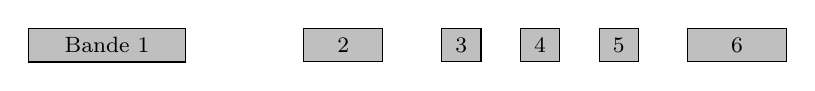
\begin{tikzpicture}
\lightspectrum

\node[draw,fill=gray!50!white,minimum width=2cm,rectangle] at (3.5, -0.2) {\footnotesize Bande 1};
\node[draw,fill=gray!50!white,minimum width=1cm,rectangle] at (6.5, -0.2) {\footnotesize 2};
\node[draw,fill=gray!50!white,minimum width=0.5cm,rectangle] at (8, -0.2) {\footnotesize 3};
\node[draw,fill=gray!50!white,minimum width=0.5cm,rectangle] at (9, -0.2) {\footnotesize 4};
\node[draw,fill=gray!50!white,minimum width=0.5cm,rectangle] at (10, -0.2) {\footnotesize 5};
\node[draw,fill=gray!50!white,minimum width=1.25cm,rectangle] at (11.5, -0.2) {\footnotesize 6};
\end{tikzpicture}
\end{document}

  }
  \caption{Exemple de répartitions de bandes spectrales dans les domaines spectraux lumineux.}
  \label{fig:multispectral}
\end{figure}

En étendant ce principe, une caméra multispectrale ou superspectrale va imager une scène non pas seulement dans les trois canaux habituels \gls{RVB} dans le domaine visible, mais dans plusieurs bandes de longueurs d'ondes plus ou moins larges pouvant se trouver aussi bien dans le visible que dans l'infrarouge ou l'ultraviolet, comme illustré dans la~\cref{fig:multispectral}. Cela conduit à des images à plusieurs canaux, généralement aux alentours d'une dizaine, qui ne sont donc pas directement visualisables par l'\oe{}il humain. Il est toutefois possible de reconstituer une image en couleurs naturelles en recomposant une image \gls{RVB} à partir des valeurs contenues dans les canaux correspondant aux longueurs d'onde du rouge, du vert et du bleu. Les acquistions multispectrales peuvent avoir des résolutions différentes en fonction des canaux. Les satellites Sentinel-2A et Sentinel-2B produisent par exemple des images à une résolution au sol de \SI{10}{\meter/\px} dans le domaine visible, mais certaines bandes, notamment dans l'infrarouge, ont des résolutions de \SI{20}{\meter/\px} ou \SI{60}{\meter/\px}. Les acquisitions couleurs satellitaires les mieux résolues spatialement ont une résolution au sol de l'ordre de \SI{50}{\centi\meter/\px}, tandis que les images aéroportées peuvent aller jusqu'à une résolution de \SI{5}{\centi\meter/\px}. Dans le cas des acquisitions satellitaires, il est courant de réaliser en simultanée une mesure multispectrale et une acquisition panchromatique, c'est-à-dire qui ne distingue pas les couleurs et produit une image en noir et blanc, à résolution supérieure. Ainsi, \gls{Pleiades} réalise à la fois une acquisition panchromatique à résolution \SI{70}{\centi\meter/\px}, rééchantillonnée à \SI{50}{\centi\meter/\px} et multispectrale à \SI{2,8}{\meter} rééchantilonnée à \SI{2}{\meter}.

\begin{figure}
  \resizebox{\textwidth}{!}{
  \documentclass{standalone}
\usepackage[utf8]{inputenc}
\usepackage[T1]{fontenc}
\usepackage{tikz}
\usepackage{pgfplots}
%%%%%%%%%%%%%%%%%%%%%%%%%%%%%%%%%%%%%%%%
%           Commandes perso            %
%%%%%%%%%%%%%%%%%%%%%%%%%%%%%%%%%%%%%%%%

%% Figures centrées, et en position 'here, top, bottom or page'
\newenvironment{figureth}{%
		\begin{figure}[htbp]
			\centering
	}{
		\end{figure}
		}


%% Tableaux centrés, et en position 'here, top, bottom or page'
\newenvironment{tableth}{%
		\begin{table}[htbp]
			\centering
			%\rowcolors{1}{coleurtableau}{coleurtableau}
	}{
		\end{table}
		}

%% Sous-figures centrées, en position 'top'
\newenvironment{subfigureth}[1]{%
	\begin{subfigure}[t]{#1}
	\centering
}{
	\end{subfigure}
}

\newcommand{\citationChap}[2]{%
	\epigraph{\og \textit{#1} \fg{}}{#2}
}

%% On commence par une page impaire quand on change le style de numérotation de pages
\let\oldpagenumbering\pagenumbering
\renewcommand{\pagenumbering}[1]{%
	\cleardoublepage
	\oldpagenumbering{#1}
}

%% Légende du dataset ISPRS
\newcommand\isprslegende{
Légende\,: \textcolor{Black}{blanc}\,: routes, \textcolor{Blue}{bleu}\,: bâtiments, \textcolor{Cerulean}{cyan}\,: végétation basse, \textcolor{OliveGreen}{vert}\,: arbres, \textcolor{Dandelion}{jaune}\,: véhicules, \textcolor{BrickRed}{rouge}\,: autre.
}

%% Dessiner des réseaux de neurones avec Tikz
\newcommand{\convlayer}[9]{%{h}{w}{d}{name}{color}{x}{y}{z}%{note w}{note h}{note d}
   \def\h{#1}
   \def\w{#2}
   \def\d{#3}
   \def\name{#4}
   \ifthenelse {\equal{#5} {}} {\def\col{white}} {\def\col{#5}}
   \def\x{#6}
   \ifthenelse {\equal{#7} {}} {\def\y{0}} {\def\y{#7}}
   \ifthenelse {\equal{#8} {}} {\def\z{0}} {\def\z{#8}}
   % ne faites pas ça chez vous !
   \ifthenelse {\equal{#9} {}} {\convlayercontinued{}{}{}} {\convlayercontinued#9}
}

\newcommand\convlayercontinued[3]{
   \def\notew{#1}
   \def\noteh{#2}
   \def\noted{#3}
   \coordinate (A) at (\x-\d/2,  \y-\h/2, \z-\w/2);
   \coordinate (B) at (\x-\d/2,  \y-\h/2, \z+\w/2);
   \coordinate (C) at (\x-\d/2,  \y+\h/2, \z+\w/2);
   \coordinate (D) at (\x-\d/2,  \y+\h/2, \z-\w/2);
   \coordinate (E) at (\x+\d/2,  \y-\h/2, \z-\w/2);
   \coordinate (F) at (\x+\d/2,  \y-\h/2, \z+\w/2);
   \coordinate (G) at (\x+\d/2,  \y+\h/2, \z+\w/2);
   \coordinate (H) at (\x+\d/2,  \y+\h/2, \z-\w/2);

    \draw [draw opacity=0.3, fill opacity=0.8, fill=\col!60!white] (A) -- (B) -- (C) -- (D) -- cycle;
    \draw [draw opacity=0.3, fill opacity=0.8, fill=\col!60!white] (A) -- (B) -- (F) -- (E) -- cycle;
    % Face haut
    %\draw [left color=\col!60!white, right color=\col!80!white, shading=axis, shading angle=180] (C) -- (D)  -- (H) -- (G) -- cycle;
    \draw [fill opacity=0.9, fill=\col!70!white] (C) -- node[rotate=45,above] {\small \name} (D) -- (H) -- (G) -- cycle;
    %\draw [fill opacity=0.9, fill=\col!70!white] (C) -- (D) -- node[above] {\small \name} (H) -- (G) -- cycle;
    % Face droite
    \draw [fill opacity=0.9, fill=\col!60!white] (E) -- node[pos=0.75,rotate=45,below] {\scriptsize \notew} (F) -- (G) --  (H) -- cycle;
    % Face avant
    %\draw [shading=axis, left color=\col!60!white, right color=\col!40!white, shading angle=-45] (B) -- node[above,rotate=90] {\scriptsize \noteh} (C) -- (G) -- (F) -- node[below] {\scriptsize \noted}  cycle;
    \draw [fill opacity=0.9, fill=\col!50!white] (B) -- node[above,rotate=90] {\scriptsize \noteh} (C) -- (G) -- (F) -- node[below] {\scriptsize \noted}  cycle;
}

\newcommand{\fclayer}[8]{%{h}{w}{name}{color}{x}{y}{z}
   \def\h{#1}
   \def\w{#2}
   \def\name{#3}
   \ifthenelse {\equal{#4} {}} {\def\col{white}} {\def\col{#4}}
   \def\x{#5}
   \def\y{#6}
   \def\z{#7}
   \def\note{#8}
   \coordinate (A) at (\x-\w/2,  \y-\h/2, \z);
   \coordinate (B) at (\x+\w/2,  \y-\h/2, \z);
   \coordinate (C) at (\x+\w/2,  \y+\h/2, \z);
   \coordinate (D) at (\x-\w/2,  \y+\h/2, \z);

   \pgfmathparse{4*\w}\let\boxwidth\pgfmathresult
    \draw [fill=\col] (A) -- node[below,text width=\boxwidth cm,align=center] {\scriptsize \note} (B) -- (C) -- (D) -- cycle;

    \node (N) at ($(A)!0.5!(B)+(0,-1,0)$) {\name};
}

\newcommand{\alexnet}[4]{%{scale}{x}{y}{z}
  \def\scale{#1}
  \def\alexx{#2}
  \def\alexy{#3}
  \def\alexz{#4}


  \def\coblue{blue!50!white}
  \def\fcgrey{gray!50!white}

  \convlayer{1.3*\scale}{1.3*\scale}{0.02*\scale}{Image}{\coblue}{\alexx}{\alexy}{\alexz}{{227}{227}{3}}
  \convlayer{1.1*\scale}{1.1*\scale}{0.08*\scale}{Conv1}{\coblue}{\alexx+0.7*\scale}{\alexy}{\alexz}{{55}{55}{96}}
  \convlayer{0.7*\scale}{0.7*\scale}{0.5*\scale}{Conv2}{\coblue}{\alexx+1.5*\scale}{\alexy}{\alexz}{{27}{27}{256}}
  \convlayer{0.5*\scale}{0.5*\scale}{0.8*\scale}{Conv3}{\coblue}{\alexx+2.6*\scale}{\alexy}{\alexz}{{13}{13}{384}}
  \convlayer{0.5*\scale}{0.5*\scale}{0.8*\scale}{Conv4}{\coblue}{\alexx+3.8*\scale}{\alexy}{\alexz}{{13}{13}{384}}
  \convlayer{0.5*\scale}{0.5*\scale}{0.5*\scale}{Conv5}{\coblue}{\alexx+4.8*\scale}{\alexy}{\alexz}{{13}{13}{256}}
  \fclayer{\scale}{0.1*\scale}{FC1}{\fcgrey}{\alexx+5.4*\scale}{\alexy}{\alexz}{4096}
  \fclayer{\scale}{0.1*\scale}{FC2}{\fcgrey}{\alexx+5.7*\scale}{\alexy}{\alexz}{4096}
  \fclayer{\scale}{0.1*\scale}{FC3}{\fcgrey}{\alexx+6.0*\scale}{\alexy}{\alexz}{1000}
}

\newcommand{\imagelayer}[7]{%{width}{x}{y}{z}{path}{text_up}{text_down}
    \pgfmathparse{#1}\let\w\pgfmathresult
    \begin{scope}[canvas is yz plane at x=#2]
     \node[transform shape] (source) at (#3, #4) {\includegraphics[angle=-90,width=\w cm]{#5}};
    \end{scope}
     \node [transform shape, rotate=45, above] at (source.east) {#6};
     \node [transform shape, rotate=45, below] at (source.west) {\scriptsize{#7}};
}

\def\fourier{\mathcal{F}}

\newcommand{\lightspectrum}{%
\pgfplotsset{
    % this *defines* a custom colormap ...
    colormap={slategraywhite}{color(0cm)=(red); color(1cm)=(red); color(2cm)=(red); color(3cm)=(red); color(4cm)=(orange); color(5cm)=(yellow); color(6cm)=(green); color(7cm)=(blue); color(8cm)=(blue); color(9cm)=(purple); color(10cm)=(purple); color(12cm)=(black)}
}
\node at (1.5, 2.7) {\small 1mm};
\node at (4, 3) {Infrarouge};
\node at (7.75, 2.7) {\small 800nm};
\node at (9, 3) {Visible};
\node at (10.5, 2.7) {\small 400nm};
\node at (12, 3) {Ultraviolet};
\node at (13.5, 2.7) {\small 10nm};
\draw[->] (1, 2.5) -- (14, 2.5);
\begin{axis}[hide axis,width=16cm,height=4cm,colormap name=slategraywhite]
\addplot[domain=20:1000,samples=1500,ultra thick, point meta=x*x,mesh]{sin(x*x/80)};
\end{axis}
}

% Union généralisée
\newcommand{\wbigcup}{\mathop{\bigcup}\displaylimits}

\newcommand{\res}[2]{#1 {\footnotesize $\pm$ #2}}
\newcommand{\bres}[2]{\textbf{#1} {\footnotesize $\pm$ #2}}
\newcommand{\bbres}[2]{\res{\textit{#1}}{#2}}

\newcommand{\drawkernel}[9]{
\begin{tikzpicture}
	\draw[step=1cm,gray!50!white,very thin] (0,0) grid (3,3);
	\kernelnode{0.5}{0.5}{#1};
	\kernelnode{0.5}{1.5}{#2};
	\kernelnode{0.5}{2.5}{#3};
	\kernelnode{1.5}{0.5}{#4};
	\kernelnode{1.5}{1.5}{#5};
	\kernelnode{1.5}{2.5}{#6};
	\kernelnode{2.5}{0.5}{#7};
	\kernelnode{2.5}{1.5}{#8};
	\kernelnode{2.5}{2.5}{#9};
\end{tikzpicture}
}

\newcommand{\kernelnode}[3]{%{x}{y}{value}
	\ifthenelse{\equal{#3}{0}}{
		\def\kcolor{gray}
	}{
		\def\kcolor{black}
	}
	\node[\kcolor] at (#1, #2) {#3};
}

\newcommand{\chapsummary}[1]{
\section*{Résumé du chapitre :}
\parbox{0.9\linewidth}{
\setlength{\parindent}{4ex}
#1}
}

\newcommand{\eqname}[1]{\tag*{\small (#1)}}

\begin{document}

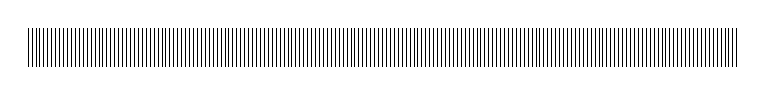
\begin{tikzpicture}
\lightspectrum

\foreach \x in {300,305,...,1200}{
\fill (\x/100, -0.5) rectangle (\x/100+0.01, 0.);
}
\end{tikzpicture}
\end{document}

  }
  \caption{Exemple de répartitions de bandes spectrales dans les domaines spectraux lumineux.}
  \label{fig:hyperspectral}
\end{figure}

L'imagerie hyperspectrale consiste à effectuer des acquisitions sur de nombreuses bandes étroites, toutes de même taille, afin de balayer de façon discrète l'ensemble du spectre lumineux réfléchi, comme illustré par la~\cref{fig:hyperspectral}. En fonction de la résolution spectrale -- souvent de l'ordre de \SI{10}{\nano\meter} -- et de la largeur du spectre considéré, le nombre de bandes peut varier de quelques dizaines à plusieurs centaines. L'avantage principale de ce type de caméra est qu'il est possible pour un pixel donné de reconstituer la courbe de l'intensité lumineuse réfléchie en fonction de la longueur d'onde. Chaque matériau réfléchit différemment la lumière en fonction de son albédo et cette information permet donc de caractériser finement la composition des objets d'intérêt observés. Toutefois, les caméras hyperspectrales ont également une résolution spatiale nettement plus faibles que les caméras \gls{RVB} ou multispectrales classiques, produisant des images à une résolution au sol d'environ \SI{1}{\meter/\px} en aérien.

Il est important de noter que ces capteurs optiques sont passifs. Ils ne reçoivent que l'énergie lumineuse réfléchie ou émise par le corps observé, ce qui restreint ce qu'il est possible de réaliser. Notamment, ces capteurs sont sensibles aux variations d'illumination et aux effets météorologiques, en particulier la couche nuageuse qui les rendre entièrement inopérationnels. Ainsi, de nombreux satellites sont eux munis de capteurs actifs qui émettent un signal et mesurent le retour de celui-ci. C'est cette approche qui est utilisée pour les satellites radar, et notamment \gls{SAR}, qui envoient une ou plusieurs ondes électromagnétiques et utilisent la mesure de l'onde réfléchie pour extraire des paramètres physiques de la zone observée.

\begin{figure}
  \resizebox{\textwidth}{!}{
  \input{Chapitre1/mnt.pdf_tex}
  }
  \caption{Schéma représentatif de la différence entre \gls{MNT} et \gls{MNE}.}
  \label{fig:mnt}
\end{figure}

En outre, le \gls{Lidar} est un capteur actif émettant une impulsion laser dont il mesure l'écho. La position du maximum d'amplitude permet de déterminer le temps d'aller-retour du signal lumineux et donc de mesurer la distance parcourue par les photons. Ces capteurs sont très utilisés aussi bien en télédétection qu'en robotique pour effectuer des relevés topographiques et la reconstruction 3D. L'inconvénient principal du \gls{Lidar} est que la mesure laser est ponctuelle et qu'il ne permet donc que de construire des nuages de points peu denses. Dans le cas du \gls{Lidar} satellitaire, les points de mesure sont généralement espacés d'environ \SI{20}{\meter}, et \SI{10}{\centi\meter} dans le cas de l'aéroporté. Une fois le nuage de points construit, il est possible d'en extraire un maillage qui modélise la topographie de la surface observée. Il est ensuite possible de rastériser ce maillage pour obtenir un \gls{MNT} ou un \gls{MNE} en fonction de la résolution. Le \gls{MNE} se distingue du \gls{MNT} en ce qu'il prend en compte les objets surélevés par-dessus la surface topographique, comme illustré par la~\cref{fig:mnt}. La différence entre ces deux modèles est appelée \gls{MNH} et correspond à la hauteur normalisée des points au-dessus du sol.

Nos travaux portent principalement sur l'utilisation de données optiques pour la cartographie automatisée, cependant, nous utiliserons également des données issues de capteurs \gls{Lidar}.

\subsection{Jeux de données en télédétection}

Il existe plusieurs jeux de données pour la classification d'images optiques de télédétection. Citons ainsi les jeux de données UC Merced~\cite{yang_bag--visual-words_2010} contenant 2 100 images aériennes dans 21 classes d'occupation des sols, Brazilian Coffe~\cite{penatti_deep_2015} d'images \gls{SPOT} pour la classification de terrains cultivés et SAT-4/SAT-6~\cite{basu_deepsat_2015} contenant respectivement 500 000 et 405 000 images aériennes pour plusieurs classes d'occupation des sols. L'inconvénient de ces jeux de données est d'une part la faible taille des images (256$\times$\SI{256}{\px} pour UC Merced et Brazilian Coffe, $28\times28$\SI{}{\px} pour SAT) et la faible quantité d'annotations. En effet, ces jeux de données, prévus pour la classification, ne peuvent que difficilement être utilisés pour la segmentation sémantique.

Cependant, plusieurs jeux de données comprenant des annotations denses ont été proposés.

\subsubsection{ISPRS 2D Semantic Labeling}

\begin{figure}[t]
		\foreach\picid in {7,21,28}{%
		\begin{subfigure}{0.33\textwidth}
			\includegraphics[angle=90,width=\textwidth]{vaihingen_top_\picid}
			\caption*{Image RVB}
		\end{subfigure}%
		\begin{subfigure}{0.33\textwidth}
			\includegraphics[angle=90,width=\textwidth]{vaihingen_ndsm_\picid}
			\caption*{\gls{MNH}}
		\end{subfigure}%
		\begin{subfigure}{0.33\textwidth}
			\includegraphics[angle=90,width=\textwidth]{vaihingen_gt_\picid}
			\caption*{Vérité terrain}
		\end{subfigure}
		}
    \caption{Images ortho-rectifiées et \gls{MNH} pour le jeu de données ISPRS Vaihingen .}
    \label{fig:isprs_vaihingen}
\end{figure}
\begin{figure}
		\foreach\picid in {3_10,6_11,7_12}{%
		\begin{subfigure}{0.33\textwidth}
			\includegraphics[width=\textwidth]{potsdam_top_\picid}
			\caption*{Image RVB}
		\end{subfigure}%
		\begin{subfigure}{0.33\textwidth}
			\includegraphics[width=\textwidth]{potsdam_ndsm_\picid}
			\caption*{\gls{MNH}}
		\end{subfigure}%
		\begin{subfigure}{0.33\textwidth}
			\includegraphics[width=\textwidth]{potsdam_gt_\picid}
			\caption*{Vérité terrain}
		\end{subfigure}
		}
	\caption{Images ortho-rectifiées et \gls{MNH} pour le jeu de données ISPRS Potsdam.}
	\label{fig:isprs_potsdam}
\end{figure}

Le jeu de données ISPRS 2D Semantic Labeling~\cite{rottensteiner_isprs_2012} est constitué de deux ensembles d'images aériennes \glsfirst{THR}. Dans les deux cas, il s'agit de scènes urbaines diposant de cinq classes d'intérêt pour la segmentation sémantique\,: surfaces imperméables (routes, parkings, trottoirs\dots), bâtiments, végétation basse, arbres et véhicules. Une classe de rejet est également définie et comprend le mobilier urbain (bancs, poubelles, conteneurs\dots) et les surfaces exotiques (terrains de basketball, zones en travaux, points d'eau).

Le jeu de données se décline en deux scènes. La première est issue d'une acquisition aéroportée sur la ville de Vaihingen (Allemagne) et comporte une mosaïque de 33 tuiles \gls{IRRV} ortho-rectifiées à une résolution de 9cm/px. L'acquisition optique est accompagnée d'une acquisition \gls{Lidar} à la même résolution, dont a été extrait un \gls{MNE}. Un \gls{MNH} pré-calculé~\cite{gerke_use_2015} dérivé du \gls{MNE} est également disponible. Les ortho-images sont fournies en format \gls{TIFF} encodés sur 8 bits, tandis que le \gls{MNE} est fourni en flottant sur 32 bits. Toutes les données ont été recalées sur la même grille de pixels. Les images ont une taille moyenne d'environ $2600\times1900$px, soit une surface d'approximativement $40 000m^2$. Vaihingen est une ville de taille moyenne (28 853 habitants en 2009), caractérisée par une urbanisation moyenne composée majoritairement de pavillons résidentiels et d'espace verts urbains.

La seconde scène est une acquisition aéroportée sur la ville de Potsdam (Allemagne) et comporte une mosaïque de 38 tuiles \gls{IRRVB} à une résolution de 5cm/px. Les tuiles présentent toutes les mêmes dimensions, à savoir $6000\times6000$px, soit une surface de $90 000m^2$. Un \gls{MNE} et un \gls{MNH} dérivé sont également fournis. Des annotations denses sont disponibles pour les mêmes classes que précédemment sur 24 images. À nouveau, l'ensemble des modalités sont recalées sur la même grille de pixels et les images sont fournies en \gls{TIFF} sur 8 bits, tandis que les modèles de surface sont fournis en flottant sur 32 bits. Potsdam est une ville urbanisée relativement grande (161 468 habitants en 2013), caractérisée par de nombreux immeubles, un réseau routier dense. À noter la présence d'un canal et de nombreux travaux de construction à la date de l'acquisition des images.

Quelques exemples représentatifs des deux acquisitions sont montrés dans les~\cref{fig:isprs_vaihingen,fig:isprs_potsdam}.

Les images dont les annotations ne sont pas rendues publiques servent à évaluer en aveugle les méthodes proposées par la communauté. La commission WG II/4 de l'\gls{ISPRS} gère ainsi un tableau de résultat public\footnote{\url{http://www2.isprs.org/commissions/comm2/wg4/vaihingen-2d-semantic-labeling-contest.html}}\footnote{\url{http://www2.isprs.org/commissions/comm2/wg4/potsdam-2d-semantic-labeling.html}}, détaillant les performances obtenues par différentes méthodes de l'état-de-l'art.

\subsubsection{Data Fusion Contest 2015}

Le jeu de données \gls{DFC} 2015~\cite{campos-taberner_processing_2016} est issu d'une compétition de fusion de données organisée par le groupe de travail \gls{GRSS} de l'\gls{IEEE}. Ce jeu de données comporte une mosaïque de 7 images couleurs ortho-rectifiées de dimensions $10 000\times10 000$ à une résolution au sol de \SI{5}{\centi\meter/\px}, soit une surface par tuile de \SI{250 000}{\meter\squared}. L'acquisition a été réalisée sur la zone portuaire de Zeebruges (Belgique) en mars 2011. Il est accompagné d'une acquisition \gls{Lidar} comprenant environ \SI{65}{points/\meter\squared} espacés chacun de \SI{10}{\centi\meter}. Les données couleurs sont fournies en \gls{TIFF} encodé sur 8 bits et les données \gls{Lidar} sont fournis rastérisées sous la forme d'un \gls{MNE} en flottant sur 32 bits, ainsi qu'un nuage de points. Des annotations denses réalisées par l'\gls{ONERA} sont disponibles pour les classes bateau, voiture, végétation basse, arbre, bâtiment, eau et surface imperméable.

Un tableau de résultats public est maintenu par l'\gls{IEEE} \gls{GRSS}\footnote{\url{http://dase.ticinumaerospace.com/}}.

\subsubsection{Data Fusion Contest 2017}

Le jeu de données \gls{DFC} 2017~\cite{tuia_2017_2017} contient une variété d'images satellites issues de Landsat et Sentinel-2, rééchantillonnées à une résolution spatiale de \SI{100}{\meter/\px} ainsi que des tuiles OpenStreetMap rastérisées à \SI{20}{\meter/\px} contenant les empreintes de bâtiments et les annotations des utilisateurs pour les classes d'occupations du sol. Des annotations partielles sont fournies contenant les 17 zones climatiques locales définies par~\citet{stewart_local_2012}.

Un tableau de résultats public est maintenu par l'\gls{IEEE} \gls{GRSS}\footnote{\url{http://dase.ticinumaerospace.com/}}.

\subsubsection{Data Fusion Contest 2018}

Le jeu de données \gls{DFC} 2018~\cite{le_saux_2018_2018} contient une image aérienne couleur ortho-rectifiée \gls{THR} à \SI{5}{\centi\meter/\px} de dimensions ..., accompagnés par une image hyperspectrale à 48 bandes à \SI{1}{\meter/\px} et un nuage de points \gls{Lidar} multispectral à \SI{0,5}{\meter/\px}, l'ensemble étant parfaitement recalé.
Des annotations partielles sont fournies pour la moitié du jeu de données sur diverses classes d'intérêt urbaines, l'autre moitié des annotations étant conservées secrètes pour l'évaluation.

Un tableau de résultats public est maintenu par l'\gls{IEEE} \gls{GRSS}\footnote{\url{http://dase.ticinumaerospace.com/}}.

\subsubsection{Inria Aerial Image Labeling}

\begin{figure}
  \foreach \picpath\picname in {chicago5_top/Ortho-image (Chicago),chicago5_gt/Vérité terrain (Chicago),vienna2_top/Ortho-image (Vienne),vienna2_gt/Vérité terrain (Vienne)}{%
  \begin{subfigure}[b]{0.25\textwidth}%
    \includegraphics[width=\textwidth]{\picpath}%
    \caption{\picname}
  \end{subfigure}%
  }
  \caption{Exemples d'images extraites de la base de données \emph{Inria Aerial Image Labeling}.}
  \label{fig:inria}
\end{figure}

Le jeu de données \emph{Inria Aerial Image Labeling}~\cite{maggiori_can_2017} contient 360 images \gls{RVB} ortho-rectifiées de taille $5000\times5000$px à une résolution de 30cm/px, soit une surface de $2,25km²$. Les images ont été compilées depuis plusieurs sources gouvernementales à des résolutions diverses. Il s'agit néanmoins systématiquement d'acquisitions aéroportées, ortho-rectifiées et rééchantillonnée à 30cm/px si besoin. Les acquisitions ont été réalisées sur 10 agglomérations de divers points du globe. La moitié des villes sont utilisées pour associées à des annotations publiques d'empreintes de bâtiments provenant de sources cadastrales. Ces images peuvent être utilisées pour l'entraînement de modèles d'extraction de bâtiments. Le reste du jeu de données est réservé à l'évaluation des modèles. Quelques images et annotations du jeu d'apprentissage sont illustrées dans la~\cref{fig:inria}.

Les organisateurs gèrent un tableau de résultats public\footnote{\url{https://project.inria.fr/aerialimagelabeling/leaderboard/}} permettant de comparer les performances obtenues par différentes méthodes.

\subsection{Classification d'images de télédétection}

\subsubsection{Approches pixelliques}

Une acquisition d'observation de la Terre est caractérisée par sa résolution spatiale. Celle-ci détermine l'unité de surface minimale au sein laquelle il devient impossible de séparer deux observations. Dans le cas d'une image, cette résolution en unité de longueur par pixel. Ainsi, une image à résolution de $10m/px$ est un ensemble d'observations, chacune effectuée sur une surface de $10\times10$m. De fait, en traitement d'images de télédétection, le pixel est l'unité atomique de surface. Par conséquent, une mesure pour 1 pixel est la mesure la plus pure disponible. Sans toutefois prétendre qu'une observation sur un pixel ne souffre pas de problèmes de mélanges (en fonction des objets d'intérêt, un pixel peut mélanger plusieurs classes hétérogènes), le pixel représente la mesure la plus fine disponible.

En première approche, il semble raisonnable de traiter le problème de cartographie comme un problème de classification des pixels. Pour ce faire, il est dans un premier temps nécessaire d'extraire des attributs du pixel. Dans le cas d'une image multispectrale, cela peut par exemple être la proportion de lumière réfléchie dans chacune des longueurs d'onde mesurées. Mais il est également possible d'y ajouter d'autres attributs : la valeur moyenne de l'intensité lumineuse ou les observations voisines. Une fois l'extraction d'attributs effectuée, il est possible de réaliser une classification.

L'avantage de cette méthode est qu'elle garantit une résolution identique à celle de la donnée.

Le premier inconvénient est que cette méthode est particulièrement susceptible au bruit. En effet, la classification s'effectuant pixel à pixel, la nature des pixels voisins n'est pas forcément prise en compte. Toutefois, les objets géographiques considérés s'étendent bien souvent sur plusieurs pixels et possèdent des propriétés géométriques particulières de connexité et de convexité. Ainsi, un pixel particulier soumis à un bruit extrême (suite à une défaillance du capteur ou à un matériau particulier), celui risque d'être mal classé de manière isolée, alors que son appartenance à une région particulière aurait pu permettre de contourner cette erreur en se basant sur des critères d'homogénéité. Ainsi la classification pixellique tend à produire des cartes exhibant un comportement de bruit poivre-et-sel.

Le second inconvénient est que le nombre de pixels croît quadratiquement avec la taille de l'image à traiter. Or, les tailles d'images considérées en télédétection peuvent rapidement conduire à devoir traiter des millions de pixels. Le problème de classification peut alors devenir intraitable sur ces images, alors que les capteurs tendent justement à s'améliorer en résolution. En particulier, la litérature s'étant intéressée à ces approches ne traite que d'images de tailles réduites~\cite{nogueira_learning_2016}, notamment dans le cadre de l'imagerie hyperspectrale~\cite{fauvel_advances_2013}.

\subsubsection{Approches par région}

\begin{figure}
\resizebox{\textwidth}{!}{%
\documentclass{standalone}
\usepackage[utf8]{inputenc}
\usepackage[T1]{fontenc}
\usepackage{tikz}
%%%%%%%%%%%%%%%%%%%%%%%%%%%%%%%%%%%%%%%%
%           Commandes perso            %
%%%%%%%%%%%%%%%%%%%%%%%%%%%%%%%%%%%%%%%%

%% Figures centrées, et en position 'here, top, bottom or page'
\newenvironment{figureth}{%
		\begin{figure}[htbp]
			\centering
	}{
		\end{figure}
		}


%% Tableaux centrés, et en position 'here, top, bottom or page'
\newenvironment{tableth}{%
		\begin{table}[htbp]
			\centering
			%\rowcolors{1}{coleurtableau}{coleurtableau}
	}{
		\end{table}
		}

%% Sous-figures centrées, en position 'top'
\newenvironment{subfigureth}[1]{%
	\begin{subfigure}[t]{#1}
	\centering
}{
	\end{subfigure}
}

\newcommand{\citationChap}[2]{%
	\epigraph{\og \textit{#1} \fg{}}{#2}
}

%% On commence par une page impaire quand on change le style de numérotation de pages
\let\oldpagenumbering\pagenumbering
\renewcommand{\pagenumbering}[1]{%
	\cleardoublepage
	\oldpagenumbering{#1}
}

%% Légende du dataset ISPRS
\newcommand\isprslegende{
Légende\,: \textcolor{Black}{blanc}\,: routes, \textcolor{Blue}{bleu}\,: bâtiments, \textcolor{Cerulean}{cyan}\,: végétation basse, \textcolor{OliveGreen}{vert}\,: arbres, \textcolor{Dandelion}{jaune}\,: véhicules, \textcolor{BrickRed}{rouge}\,: autre.
}

%% Dessiner des réseaux de neurones avec Tikz
\newcommand{\convlayer}[9]{%{h}{w}{d}{name}{color}{x}{y}{z}%{note w}{note h}{note d}
   \def\h{#1}
   \def\w{#2}
   \def\d{#3}
   \def\name{#4}
   \ifthenelse {\equal{#5} {}} {\def\col{white}} {\def\col{#5}}
   \def\x{#6}
   \ifthenelse {\equal{#7} {}} {\def\y{0}} {\def\y{#7}}
   \ifthenelse {\equal{#8} {}} {\def\z{0}} {\def\z{#8}}
   % ne faites pas ça chez vous !
   \ifthenelse {\equal{#9} {}} {\convlayercontinued{}{}{}} {\convlayercontinued#9}
}

\newcommand\convlayercontinued[3]{
   \def\notew{#1}
   \def\noteh{#2}
   \def\noted{#3}
   \coordinate (A) at (\x-\d/2,  \y-\h/2, \z-\w/2);
   \coordinate (B) at (\x-\d/2,  \y-\h/2, \z+\w/2);
   \coordinate (C) at (\x-\d/2,  \y+\h/2, \z+\w/2);
   \coordinate (D) at (\x-\d/2,  \y+\h/2, \z-\w/2);
   \coordinate (E) at (\x+\d/2,  \y-\h/2, \z-\w/2);
   \coordinate (F) at (\x+\d/2,  \y-\h/2, \z+\w/2);
   \coordinate (G) at (\x+\d/2,  \y+\h/2, \z+\w/2);
   \coordinate (H) at (\x+\d/2,  \y+\h/2, \z-\w/2);

    \draw [draw opacity=0.3, fill opacity=0.8, fill=\col!60!white] (A) -- (B) -- (C) -- (D) -- cycle;
    \draw [draw opacity=0.3, fill opacity=0.8, fill=\col!60!white] (A) -- (B) -- (F) -- (E) -- cycle;
    % Face haut
    %\draw [left color=\col!60!white, right color=\col!80!white, shading=axis, shading angle=180] (C) -- (D)  -- (H) -- (G) -- cycle;
    \draw [fill opacity=0.9, fill=\col!70!white] (C) -- node[rotate=45,above] {\small \name} (D) -- (H) -- (G) -- cycle;
    %\draw [fill opacity=0.9, fill=\col!70!white] (C) -- (D) -- node[above] {\small \name} (H) -- (G) -- cycle;
    % Face droite
    \draw [fill opacity=0.9, fill=\col!60!white] (E) -- node[pos=0.75,rotate=45,below] {\scriptsize \notew} (F) -- (G) --  (H) -- cycle;
    % Face avant
    %\draw [shading=axis, left color=\col!60!white, right color=\col!40!white, shading angle=-45] (B) -- node[above,rotate=90] {\scriptsize \noteh} (C) -- (G) -- (F) -- node[below] {\scriptsize \noted}  cycle;
    \draw [fill opacity=0.9, fill=\col!50!white] (B) -- node[above,rotate=90] {\scriptsize \noteh} (C) -- (G) -- (F) -- node[below] {\scriptsize \noted}  cycle;
}

\newcommand{\fclayer}[8]{%{h}{w}{name}{color}{x}{y}{z}
   \def\h{#1}
   \def\w{#2}
   \def\name{#3}
   \ifthenelse {\equal{#4} {}} {\def\col{white}} {\def\col{#4}}
   \def\x{#5}
   \def\y{#6}
   \def\z{#7}
   \def\note{#8}
   \coordinate (A) at (\x-\w/2,  \y-\h/2, \z);
   \coordinate (B) at (\x+\w/2,  \y-\h/2, \z);
   \coordinate (C) at (\x+\w/2,  \y+\h/2, \z);
   \coordinate (D) at (\x-\w/2,  \y+\h/2, \z);

   \pgfmathparse{4*\w}\let\boxwidth\pgfmathresult
    \draw [fill=\col] (A) -- node[below,text width=\boxwidth cm,align=center] {\scriptsize \note} (B) -- (C) -- (D) -- cycle;

    \node (N) at ($(A)!0.5!(B)+(0,-1,0)$) {\name};
}

\newcommand{\alexnet}[4]{%{scale}{x}{y}{z}
  \def\scale{#1}
  \def\alexx{#2}
  \def\alexy{#3}
  \def\alexz{#4}


  \def\coblue{blue!50!white}
  \def\fcgrey{gray!50!white}

  \convlayer{1.3*\scale}{1.3*\scale}{0.02*\scale}{Image}{\coblue}{\alexx}{\alexy}{\alexz}{{227}{227}{3}}
  \convlayer{1.1*\scale}{1.1*\scale}{0.08*\scale}{Conv1}{\coblue}{\alexx+0.7*\scale}{\alexy}{\alexz}{{55}{55}{96}}
  \convlayer{0.7*\scale}{0.7*\scale}{0.5*\scale}{Conv2}{\coblue}{\alexx+1.5*\scale}{\alexy}{\alexz}{{27}{27}{256}}
  \convlayer{0.5*\scale}{0.5*\scale}{0.8*\scale}{Conv3}{\coblue}{\alexx+2.6*\scale}{\alexy}{\alexz}{{13}{13}{384}}
  \convlayer{0.5*\scale}{0.5*\scale}{0.8*\scale}{Conv4}{\coblue}{\alexx+3.8*\scale}{\alexy}{\alexz}{{13}{13}{384}}
  \convlayer{0.5*\scale}{0.5*\scale}{0.5*\scale}{Conv5}{\coblue}{\alexx+4.8*\scale}{\alexy}{\alexz}{{13}{13}{256}}
  \fclayer{\scale}{0.1*\scale}{FC1}{\fcgrey}{\alexx+5.4*\scale}{\alexy}{\alexz}{4096}
  \fclayer{\scale}{0.1*\scale}{FC2}{\fcgrey}{\alexx+5.7*\scale}{\alexy}{\alexz}{4096}
  \fclayer{\scale}{0.1*\scale}{FC3}{\fcgrey}{\alexx+6.0*\scale}{\alexy}{\alexz}{1000}
}

\newcommand{\imagelayer}[7]{%{width}{x}{y}{z}{path}{text_up}{text_down}
    \pgfmathparse{#1}\let\w\pgfmathresult
    \begin{scope}[canvas is yz plane at x=#2]
     \node[transform shape] (source) at (#3, #4) {\includegraphics[angle=-90,width=\w cm]{#5}};
    \end{scope}
     \node [transform shape, rotate=45, above] at (source.east) {#6};
     \node [transform shape, rotate=45, below] at (source.west) {\scriptsize{#7}};
}

\def\fourier{\mathcal{F}}

\newcommand{\lightspectrum}{%
\pgfplotsset{
    % this *defines* a custom colormap ...
    colormap={slategraywhite}{color(0cm)=(red); color(1cm)=(red); color(2cm)=(red); color(3cm)=(red); color(4cm)=(orange); color(5cm)=(yellow); color(6cm)=(green); color(7cm)=(blue); color(8cm)=(blue); color(9cm)=(purple); color(10cm)=(purple); color(12cm)=(black)}
}
\node at (1.5, 2.7) {\small 1mm};
\node at (4, 3) {Infrarouge};
\node at (7.75, 2.7) {\small 800nm};
\node at (9, 3) {Visible};
\node at (10.5, 2.7) {\small 400nm};
\node at (12, 3) {Ultraviolet};
\node at (13.5, 2.7) {\small 10nm};
\draw[->] (1, 2.5) -- (14, 2.5);
\begin{axis}[hide axis,width=16cm,height=4cm,colormap name=slategraywhite]
\addplot[domain=20:1000,samples=1500,ultra thick, point meta=x*x,mesh]{sin(x*x/80)};
\end{axis}
}

% Union généralisée
\newcommand{\wbigcup}{\mathop{\bigcup}\displaylimits}

\newcommand{\res}[2]{#1 {\footnotesize $\pm$ #2}}
\newcommand{\bres}[2]{\textbf{#1} {\footnotesize $\pm$ #2}}
\newcommand{\bbres}[2]{\res{\textit{#1}}{#2}}

\newcommand{\drawkernel}[9]{
\begin{tikzpicture}
	\draw[step=1cm,gray!50!white,very thin] (0,0) grid (3,3);
	\kernelnode{0.5}{0.5}{#1};
	\kernelnode{0.5}{1.5}{#2};
	\kernelnode{0.5}{2.5}{#3};
	\kernelnode{1.5}{0.5}{#4};
	\kernelnode{1.5}{1.5}{#5};
	\kernelnode{1.5}{2.5}{#6};
	\kernelnode{2.5}{0.5}{#7};
	\kernelnode{2.5}{1.5}{#8};
	\kernelnode{2.5}{2.5}{#9};
\end{tikzpicture}
}

\newcommand{\kernelnode}[3]{%{x}{y}{value}
	\ifthenelse{\equal{#3}{0}}{
		\def\kcolor{gray}
	}{
		\def\kcolor{black}
	}
	\node[\kcolor] at (#1, #2) {#3};
}

\newcommand{\chapsummary}[1]{
\section*{Résumé du chapitre :}
\parbox{0.9\linewidth}{
\setlength{\parindent}{4ex}
#1}
}

\newcommand{\eqname}[1]{\tag*{\small (#1)}}

\begin{document}

\begin{tikzpicture}[]
\usetikzlibrary{3d}
\usetikzlibrary{calc}
\usetikzlibrary{arrows.meta, bending}

\coordinate (input) at (0, 2);
\coordinate (seg) at (0,-3);
\coordinate (patches) at (5, 0);
\coordinate (net) at (11.5, 0);
\coordinate (features) at (16.5, 0);
\coordinate (classifier) at (19, 0);
\coordinate (map) at (24, 0);

\node (in_fig) at (input) {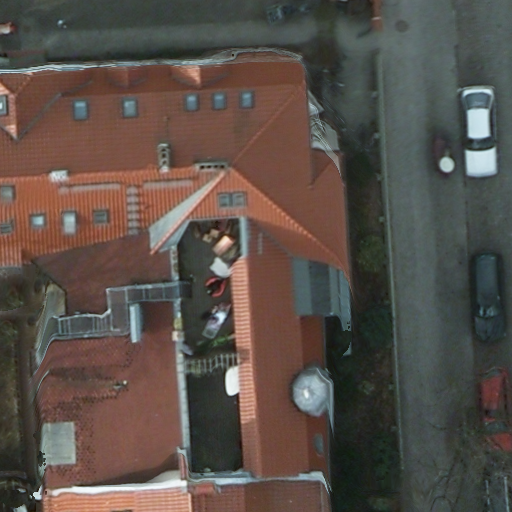
\includegraphics[width=3cm]{orthohr_rgb}};
\node[yshift=4pt] at (in_fig.north) {Image initiale};

\node (seg_fig) at (seg) {\includegraphics[width=3cm]{orthohr_rgb_slic}};
\node[yshift=-4pt] at (seg_fig.south) {Image segmentée};

\draw[ultra thick,->] ([xshift=0.8cm]in_fig.south) to node[left]{\small segmentation} ([xshift=0.8cm]seg_fig.north);

\node (large) at ($ (patches)+(0,2.5)$) {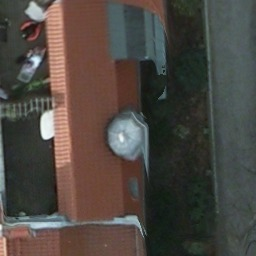
\includegraphics[width=2cm]{large}};
\node[yshift=-3pt] at (large.south) {contexte};
\node (medium) at (patches) {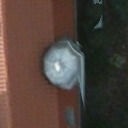
\includegraphics[width=2cm] {medium}};
\node[yshift=-3pt] at (medium.south) {contexte};
\node (ndsm) at ($ (patches)-(0,2.5) $) {\includegraphics[width=2cm]{ndsm}};
\node[yshift=-3pt] at (ndsm.south) {MNH};

\fill[line width=3pt,draw=red!95!black,fill=cyan!80!white,fill opacity=0.5,shading=axis, shading angle=135] (seg_fig.east) ++(-1.6,-1.1) --  +(0.6,0) -- +(0.6,0.6) -- +(0,0.6) -- cycle;

\draw (seg_fig.east) edge[in=180,out=0,->] (medium.west);
\draw (seg_fig.east) edge[in=180,out=0,->,looseness=0.8] (large.west);
\draw (seg_fig.east) edge[in=180,out=0,->] (ndsm.west);

\node[align=center] at ($ (patches)-(0,4.5) $) {Entrées multi-sources\\ et multi-échelles};

\node (net_fig) at (net) {\includegraphics[width=8cm]{../alexnet}};
\node at ($ (net) - (0,2)$) {CNN pré-entraîné};

\draw (large.east) edge[in=180,out=0,->] ([yshift=8pt]net_fig.west);
\draw (medium.east) edge[in=180,out=0,->] (net_fig.west);
\draw (ndsm.east) edge[in=180,out=0,->] ([yshift=-8pt]net_fig.west);

\coordinate (A) at ($ (features)+(0,-3,-0.5)$);
\coordinate (B) at ($ (features)+(0,3,-0.5)$);
\coordinate (C) at ($ (features)+(0.5,3,-0.5)$);
\coordinate (D) at ($ (features)+(0.5,-3,-0.5)$);
\coordinate (E) at ($ (features)+(0,-3,0)$);
\coordinate (F) at ($ (features)+(0,3,0)$);
\coordinate (G) at ($ (features)+(0.5,3,0)$);
\coordinate (H) at ($ (features)+(0.5,-3,0)$);

\coordinate (I) at ($ (E)!0.33!(F)$);
\coordinate (J) at ($ (E)!0.66!(F)$);
\coordinate (K) at ($ (H)!0.33!(G)$);
\coordinate (L) at ($ (H)!0.66!(G)$);
\coordinate (M) at ($ (D)!0.33!(C)$);
\coordinate (N) at ($ (D)!0.66!(C)$);

\def\grey{gray!40!white}
\draw[fill=\grey] (A) -- (B) -- (C) -- (D) -- cycle;
\draw[fill=\grey!60!white] (E) -- (F) -- (G) -- (H) -- cycle;
\draw[fill=\grey] (B) -- (C) -- (G) -- (F) -- cycle;
\draw[fill=\grey] (C) -- (D) -- (H) -- (G) -- cycle;
\draw[dotted,thick] (I) -- (K) -- (M);
\draw[dotted,thick] (J) -- (L) -- (N);
\node[align=center] at ($ (features) - (0,4.5)$) {Caractéristiques\\ profondes};

\draw ([yshift=-8pt]net_fig.east) edge[out=0,in=180,->] ($(I)!0.5!(E)$);
\draw ([yshift=8pt]net_fig.east) edge[out=0,in=180,->] ($(J)!0.5!(F)$);
\draw (net_fig.east) edge[out=0,in=180,->] ($(F)!0.5!(E)$);

\coordinate (c_A) at ($ (classifier) + (-1,1.5)$);
\coordinate (c_B) at ($ (classifier) + (-1,-1.5)$);
\coordinate (c_C) at ($ (classifier) + (1,-1.5)$);
\coordinate (c_D) at ($ (classifier) + (1,1.5)$);
\coordinate (c_top) at ($(c_A)!0.5!(c_D)$);
\coordinate (c_bottom) at ($ (c_B)!0.5!(c_C)$);
\filldraw[fill=yellow!50!white] (c_A) rectangle (c_C);


\newcommand\children[3]{
\coordinate (#1_c1) at ($(#1)!0.5!(#2)$);
\filldraw[fill=black] (#1_c1) circle (0.08);
\draw (#1) -- (#1_c1);
\coordinate (#1_c2) at ($(#1)!0.5!(#3)$);
\filldraw[fill=black] (#1_c2) circle (0.08);
\draw (#1) -- (#1_c2);
}

\coordinate (c_center) at ($(c_A)!0.5!(c_C)$);
\coordinate (c_center) at ($(c_center)!0.75!(c_top)$);
\filldraw[fill=black] (c_center) circle (0.1);
\coordinate (n1) at ($(c_center)!0.25!(c_B)$);
\filldraw[fill=black] (n1) circle (0.08);
\draw (c_center) -- (n1);
\coordinate (n2) at ($(c_center)!0.25!(c_C)$);
\filldraw[fill=black] (n2) circle (0.08);
\draw (c_center) -- (n2);

\children{n2}{c_bottom}{c_C}
\children{n2_c2}{c_bottom}{c_C}

\children{n1}{c_B}{c_bottom}
\children{n1_c1}{c_B}{c_bottom}

\node at ($(classifier) - (0,2)$) {Classifieur};

\draw ($(G)!0.5!(H)$) edge[ultra thick,in=180,out=0,->]  ($(c_A)!0.5!(c_B)$);

\node (map_fig) at (map) {\includegraphics[width=3cm]{gt_boundaries}};
\node[yshift=-4pt] at (map_fig.south) {Carte sémantique};
\fill[line width=3pt,draw=red!95!black,fill=cyan!50!white,fill opacity=0.2] (map_fig.east) ++(-1.6,-1.1) --  +(0.6,0) -- +(0.6,0.6) -- +(0,0.6) -- cycle;

\draw ($(c_C)!0.5!(c_D)$) edge[ultra thick,in=180,out=0,->] node[yshift=4pt,above]{Prédiction} node[yshift=-4pt,below]{\color{blue} ``Bâtiment''} (map_fig.west);

\end{tikzpicture}

\end{document}

}
\caption{Segmentation sémantique par régions d'une image aérienne. Chaque région de l'image segmentée est classifiée à partir de caractéristiques profondes extraites d'un réseau convolutif pré-entraîné.}
\label{fig:framework}
\end{figure}

Compte-tenu de l'explosion du coût calculatoire des classifications pixelliques sur des images \gls{HR}, \gls{THR} et \gls{EHR}, plusieurs travaux se sont penchés sur des approches considérant d'autres découpages de l'image que la grille de pixels. En particulier, il est envisageable de regrouper des pixels similaires dans des régions homogènes. La similarité peut alors uniquement se fonder sur des critères statistiques liées aux valeurs des pixels, ou à des critères sémantiques. Dans le premier cas, on parlera de ``superpixels'' et dans le second cas de ``segmentation''.

L'avantage de ces méthodes est qu'elles permettent de regrouper des pixels d'apparence similaire dans une même région. Or, on peut raisonnablement s'attendre à ce que des pixels spatiallement et spectralement proches possèdent la même sémantique, c'est-à-dire que l'on puisse les associer à la même classe d'intérêt. Dans ce cas, plutôt que de réaliser la classification pixel par pixel, il est possible de ne réaliser qu'une seule extraction d'attributs pour l'ensemble de la région homogène et de ne faire qu'une unique prédiction. Ainsi, dans le cas d'une image de dimensions $1500\times1500$ segmentée en $20 000$ régions, on peut alors cartographier l'image en classifiant $20 000$ régions plutôt qu'en classifiant \nombre{2250000} pixels, soit ungain en temps de calcul d'un facteur $112$ (segmentation exclue).

De nombreux algorithmes de segmentation ont été proposés, aussi bien dans la communauté télédétection que dans la communauté vision par ordinateur. Ces algorithmes de segmentation viennent partitionner l'ensemble des pixels de façon non-supervisée. Une fois ce partitionnement effectué, il est possible d'extraire des attributs pour chaque région et d'entraîner un classifieur de la façon usuelle, l'inférence se faisant de façon analogue. Ce procéde est illustré dans la~\cref{fig:framework}.

L'avantage principal de ces méthodes est de grandement réduire la complexité calculatoire. Notamment, lorsque l'image augmente de résolution spatiale, de nombreuses régions conservent leur homogénéité et il est ainsi très avantageux de les conserver regroupées\,: l'augmentation de la résolution ne nécessite pas obligatoirement une évolution quadratique du nombre de régions segmentées. Ces approches ont ainsi été utilisées avec succès dans le cadre de la segmentation sémantique d'images aériennes \gls{THR}~\cite{lagrange_benchmarking_2015,vargas_superpixel-based_2014}.

On peut noter que traiter l'image par une fenêtre glissante ou même par une grille de pixels correspond à des cas particuliers de classification par région.

Approches par patch, puis par segments, puis FCN

En hyperspectral, approches pixelliques car images petites


\bibliographystyle{plainnat}
\bibliography{Chapitre1/Historique}
